\documentclass[12pt]{article}
\usepackage[utf8]{inputenc}
\usepackage[T1]{fontenc}
\usepackage[english]{babel}
\usepackage{graphicx}
\usepackage{geometry}
\usepackage{longtable}
\usepackage{array}
\usepackage{amssymb}
\usepackage{booktabs}
\usepackage[scale=1]{sourcecodepro}
\usepackage{tabularx}
\usepackage{parskip}  % mejora la separación entre párrafos
\usepackage{cite}          % Para que las citas se ordenen bien (por ejemplo [1], [2], [3] => [1]–[3])
\usepackage{xurl}          % Para incluir URLs largas con saltos de línea en cualquier carácter
\usepackage{hyperref}      % Enlaces clicables (opcional pero útil)
\usepackage{float}
\usepackage{multirow}
\usepackage[table,xcdraw]{xcolor}
\usepackage{pdfpages}
\usepackage{siunitx}
\usepackage{titlesec}
\usepackage{listings}
\usepackage{amsmath}
\usepackage{caption}
\captionsetup{font=small, width=0.94\textwidth, labelfont=bf, labelsep=period}
\usepackage{tikz}
\usetikzlibrary{arrows.meta,positioning,fit,backgrounds,calc}

% --- Definición de colores para Python ---
\definecolor{codegreen}{rgb}{0.15,0.55,0.15}
\definecolor{codegray}{rgb}{0.5,0.5,0.5}
\definecolor{codepurple}{rgb}{0.60,0.15,0.70}
\definecolor{codeblue}{rgb}{0.13,0.35,0.70}
\definecolor{backcolor}{rgb}{0.98,0.98,0.98}
\definecolor{framecolor}{rgb}{0.85,0.85,0.85}

% --- Estilo general de Python ---
\lstdefinestyle{pythonstyle}{
    language=Python,
    backgroundcolor=\color{backcolor},
    commentstyle=\color{codegreen}\itshape,
    keywordstyle=\color{codeblue}\bfseries,
    numberstyle=\tiny\color{codegray},
    stringstyle=\color{codepurple},
    basicstyle=\ttfamily\footnotesize,   % Tamaño adecuado para evitar saltos de línea innecesarios
    breakatwhitespace=false,
    breaklines=true,                    % Parte líneas largas automáticamente
    postbreak=\mbox{\textcolor{codegray}{$\hookrightarrow$}\space}, % Flecha indicadora de salto de línea
    captionpos=t,                       % Posición del título (arriba)
    keepspaces=true,
    numbers=left,                       % Números de línea a la izquierda
    numbersep=8pt,
    showspaces=false,
    showstringspaces=false,
    showtabs=false,
    tabsize=4,
    frame=lines,                        % Línea arriba y abajo del bloque (limpio y elegante)
    rulecolor=\color{framecolor},
    % Soporte para tildes y caracteres en español dentro de los comentarios:
    literate=
        {á}{{\'a}}1 {é}{{\'e}}1 {í}{{\'i}}1 {ó}{{\'o}}1 {ú}{{\'u}}1
        {Á}{{\'A}}1 {É}{{\'E}}1 {Í}{{\'I}}1 {Ó}{{\'O}}1 {Ú}{{\'U}}1
        {ñ}{{\~n}}1 {Ñ}{{\~N}}1 {¿}{{?`}}1 {¡}{{!`}}1
}

\makeatletter
\newcounter{subsubsubsection}[subsubsection]
\renewcommand{\thesubsubsubsection}{\thesubsubsection.\arabic{subsubsubsection}}
\def\toclevel@subsubsubsection{4}
\makeatother

\titleclass{\subsubsubsection}{straight}[\subsubsection]
\titleformat{\subsubsubsection}{\normalfont\normalsize\bfseries}{\thesubsubsubsection}{1em}{}
\titlespacing*{\subsubsubsection}{0pt}{3.25ex plus 1ex minus .2ex}{1.5ex plus .2ex}

\setcounter{secnumdepth}{4}
\setcounter{tocdepth}{4}

% Compatibility alias so unnumbered \chapter* and ToC chapter entries work cleanly in article class
\makeatletter
\def\toclevel@chapter{1}
\let\l@chapter\l@section
\providecommand{\chapter}{\@ifstar{\@schapter}{\@chapter}}
\def\@schapter#1{\section*{#1}}
\def\@chapter#1{\section{#1}}
\makeatother

\newcounter{appcount}
\renewcommand{\theappcount}{\Alph{appcount}}
\renewcommand{\theHappcount}{appendix.\theappcount}

\newcommand{\myappendix}[1]{%
    \clearpage
    \phantomsection
    \refstepcounter{appcount}%
    \setcounter{section}{\value{appcount}}%
    \setcounter{subsection}{0}%
    \setcounter{subsubsection}{0}%
    \section*{Appendix \theappcount: #1}%
    \addcontentsline{toc}{section}{Appendix \theappcount: #1}%
    % Opcional: Reinicia y numera figuras, tablas y ecuaciones como A.1, A.2...
    \setcounter{figure}{0}%
    \renewcommand{\thefigure}{\theappcount.\arabic{figure}}%
    \setcounter{table}{0}%
    \renewcommand{\thetable}{\theappcount.\arabic{table}}%
    \setcounter{equation}{0}%
    \renewcommand{\theequation}{\theappcount.\arabic{equation}}%
}

\newcounter{annexcount}
\renewcommand{\theannexcount}{\Alph{annexcount}}
\renewcommand{\theHannexcount}{annex.\theannexcount}

\newcommand{\myannex}[1]{%
    \clearpage
    \phantomsection
    \refstepcounter{annexcount}%
    \setcounter{section}{\value{annexcount}}%
    \setcounter{subsection}{0}%
    \setcounter{subsubsection}{0}%
    \section*{\raggedright Annex \theannexcount: #1}%
    \addcontentsline{toc}{section}{Annex \theannexcount: #1}%
    % Opcional: Reinicia y numera figuras y tablas como A.1, A.2...
    \setcounter{figure}{0}%
    \renewcommand{\thefigure}{\theannexcount.\arabic{figure}}%
    \setcounter{table}{0}%
    \renewcommand{\thetable}{\theannexcount.\arabic{table}}%
}

% --- Licencia Creative Commons ---
\usepackage[
    type={CC},
    modifier={by-nc-nd},
    version={4.0}
]{doclicense}


\hypersetup{
    unicode=false,          
    colorlinks=true,       
    linkcolor=blue!70,        
    citecolor=cyan!88!black,        
    filecolor=cyan,         
    urlcolor=blue       
}
\geometry{margin=2.5cm}

\begin{document}
%--------------------------%
% Portada
%--------------------------%
\pagenumbering{roman}
\thispagestyle{empty}
\begin{center}



\includegraphics[width=0.55\textwidth]{Images/Tec.png} \\[0.35cm]
{\large\textbf{Costa Rica Institute of Technology (Tecnol\'ogico de Costa Rica)}} \\

\vfill

{\large School of Physics} \\
{\large Academic Unit of Engineering Physics} \\
{\large Final Graduation Project} \\
{\large Thesis submitted in partial fulfillment of the requirements for the Engineering Physics Licentiate Degree} \\[0.7cm]

{\LARGE \textbf{
Analysis of magnetohydrodynamic oscillations at Heliotron J with Python
}}

\vfill
\textbf{Student:} \\
Kevin Enrique Rishor Villalobos \\
2022093578 \\
krishor@estudiantec.cr\\
(+506) 8658-8959


\vfill


Thesis Advisor: Ph.D. Iván Vargas Blanco\\
Reader: M.Sc. Ricardo Solano Piedra\\  [0.7cm]

\textbf{Involved Institutions:} \\
Heliotron J Project, Institute of Advanced Energy, \\ Kyoto University, Uji Campus, Kyoto, Japan \\
\includegraphics[width=0.15\textwidth]{"Images/Heliotron logo.jpg"} \hspace{0.3cm}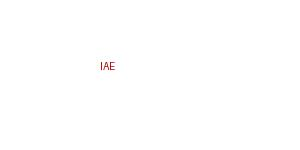
\includegraphics[width=0.175\textwidth]{Images/IAE.jpg}  \\[0.2cm]

Plasma Laboratory for Fusion Energy and Applications (PlasmaTEC), \\ Costa Rica Institute of Technology \\ [0.2cm]

\includegraphics[width=0.48\textwidth]{Images/plasmas cuadro.jpg}\\[0.5cm]

November, 2026\\
Cartago, Costa Rica\\






\vfill

\end{center} % Cierre de la portada

% --- Indices & List of Symbols and Abbreviations ---
\clearpage
\phantomsection
\tableofcontents
\thispagestyle{plain}

\clearpage
\phantomsection
\addcontentsline{toc}{section}{List of Figures}
\listoffigures
\thispagestyle{plain}

\clearpage
\phantomsection
\addcontentsline{toc}{section}{List of Tables}
\listoftables
\thispagestyle{plain}

\clearpage
\phantomsection
\addcontentsline{toc}{section}{List of Symbols and Abbreviations}
\section*{List of Symbols and Abbreviations}
\thispagestyle{plain}

\noindent\textbf{Main Physical and Mathematical Symbols}
\par\vspace{0.25em}
\noindent{\footnotesize\setlength{\tabcolsep}{3.5pt}%
\renewcommand{\arraystretch}{0.96}%
\begin{tabularx}{\textwidth}{@{}l >{\raggedright\arraybackslash}X l >{\raggedright\arraybackslash}X@{}}
\toprule
\textbf{Symbol} & \textbf{Description} & \textbf{Symbol} & \textbf{Description} \\
\midrule
$\alpha, \alpha_{\mathrm{adj}}$ & Nominal and Bonferroni levels & $I_{\mathrm{ECE}}$ & Uncalibrated ECE intensity ($\mathrm{a.u.}$) \\
$\beta$ & Kinetic-to-magnetic pressure ratio & $I_p$ & Toroidal plasma current ($\mathrm{A}$) \\
$\gamma, \gamma^2, \gamma_{95}^2$ & Exponent ($\gamma$); coherence and $95\,\%$ floor & $k_B$ & Boltzmann constant ($\mathrm{J/K}$) \\
$\Delta f, \Delta f_{\mathrm{IF}}$ & STFT bin width ($\mathrm{Hz}$); IF width ($\mathrm{GHz}$) & $k_\parallel$ & Parallel wavenumber ($\mathrm{m^{-1}}$) \\
$\Delta\Phi_{\mathrm{dia}}$ & Excluded diamagnetic flux ($\mathrm{Wb}$) & $K, K_{\mathrm{min}}, K_{\mathrm{eff}}$ & Sub-ensemble, min., and effective counts \\
$\varepsilon_0$ & Vacuum permittivity ($\mathrm{F/m}$) & $L, L_{\mathrm{sys}}$ & Helical pole ($L = 1$); system size ($\mathrm{m}$) \\
$\zeta$ & Toroidal flux-surface angle ($\mathrm{rad}$) & $m, m_1, m_2$ & Poloidal mode numbers (single/dual) \\
$\theta, \theta_j$ & Poloidal and sensor angles ($\mathrm{rad}$) & $m_e, m_i, m_p$ & Electron, ion, and proton masses ($\mathrm{kg}$) \\
$\iota$ & Rotational transform ($\mathrm{rad}$, $\iota/2\pi = 1/q$) & $m_{\mathrm{eff}}$ & Effective ion mass ($\mathrm{kg}$, rel.\ to $m_p$) \\
$\lambda_D$ & Debye shielding length ($\mathrm{m}$) & $M$ & Toroidal field period count ($M = 4$) \\
$\mu_0$ & Vacuum permeability ($\mathrm{H/m}$) & $n$ & Toroidal mode no.; bulk density ($\mathrm{m^{-3}}$) \\
$\rho, \Delta\rho$ & Normalized radius ($r/a$); ECE width & $n_e, n_i$ & Electron and ion densities ($\mathrm{m^{-3}}$) \\
$\rho_x(k)$ & Sample autocorrelation at lag $k$ & $N, N_{\mathrm{fft}}, N_{\mathrm{seg}}$ & Sample, transform, and segment counts \\
$\sigma, \hat{\sigma}_{\mathrm{MAD}}$ & Standard deviation and MAD ($\mathrm{V}$) & $N_{\mathrm{eff}}, N_{\mathrm{est}}$ & Effective and estimation segment counts \\
$\tau, \Delta\tau$ & Time lag or radial delay ($\mathrm{s}$) & $N_{\mathrm{null}}, N_{\mathrm{pairs}}$ & Surrogate and toroidal-pair counts \\
$\tau_E, \tau_{\mathrm{opt}}$ & Confinement time ($\mathrm{s}$); optical depth & $N_{\mathrm{probes}}, N_{\mathrm{sub}}$ & Coil count and sub-ensemble realizations \\
$\phi, \Delta\phi$ & Signal phase ($\phi_j$); phase lag ($\mathrm{rad}$) & $N A$ & Mirnov coil effective area-turns ($\mathrm{m^2}$) \\
$\varphi, \Delta\varphi$ & Coil angle and optical phase ($\mathrm{rad}$) & $p, p_{\mathrm{adj}}, p_{\mathrm{surr}}$ & Raw, adj., surr.\ $p$; pressure ($\mathrm{Pa}$) \\
$\psi(t)$ & Complex Morlet analyzing wavelet & $p_{\mathrm{emp}}, p_{\mathrm{sliding}}$ & Empirical and sliding-window $p$-values \\
$\omega, \omega_0$ & Angular ($\mathrm{rad/s}$); Morlet central freq. & $P(f, t)$ & Power spectral density ($\mathrm{V^2/Hz}$) \\
$\omega_{\mathrm{BAE}}, \omega_{pe}$ & BAE and electron plasma freq. ($\mathrm{rad/s}$) & $P_{\mathrm{NBI}}$ & NBI heating power ($\mathrm{W}$) \\
$a$ & Average plasma minor radius ($\mathrm{m}$) & $q$ & Safety factor ($2\pi/\iota$, dimensionless) \\
$A(t)$ & Analytic amplitude envelope ($\mathrm{V}$) & $q_{2.5}, q_{97.5}$ & Empirical $2.5\text{th}$ and $97.5\text{th}$ percentiles \\
$b^2, b_0$ & Squared bicoherence and $b^2_\infty$ intercept & $r$ & Pearson $r$ ($r_{\mathrm{car}}, r_{\mathrm{env}}, r_{\mathrm{partial}}$); radius ($\mathrm{m}$) \\
$B, B_0$ & Magnetic and equilibrium fields ($\mathrm{T}$) & $r_{\mathrm{circ}}$ & Circular concentration ($\in [0, 1]$) \\
$\tilde{B}_\theta, \dot{B}$ & Poloidal field ($\mathrm{T}$) and $\mathrm{d}\tilde{B}_\theta/\mathrm{d}t$ ($\mathrm{T/s}$) & $R_0, R^2$ & Major radius ($\mathrm{m}$); coeff.\ of determination \\
$B(f_1, f_2)$ & Auto-bispectrum ($\mathrm{V^3/Hz^3}$) & $R_{xy}(\tau)$ & Lagged cross-correlation function \\
$c, c_s$ & Light and ion sound speeds ($\mathrm{m/s}$) & $t, t_0$ & Time and ECH-off reference ($\mathrm{s}$) \\
$C$ & Finite-sample $1/K$ bias slope & $T$ & STFT window ($\mathrm{s}$); thermal $k_B T$ ($\mathrm{keV}$) \\
$e$ & Elementary charge ($\mathrm{C}$) & $T_e, T_i$ & Electron and ion temperatures ($\mathrm{K}, \mathrm{keV}$) \\
$f, f_0, f_c$ & Mode, peak, and filter cutoff freq. ($\mathrm{Hz}$) & $T_{e,\mathrm{dia}}, \tilde{T}_e$ & Diamagnetic proxy and fluctuating $T_e$ \\
$f_1, f_2, f_3$ & Triad frequencies ($f_3 = f_1 \pm f_2$, $\mathrm{Hz}$) & $v_A$ & Shear-Alfv\'en wave speed ($\mathrm{m/s}$) \\
$f_{\mathrm{BAE}}, f_{\mathrm{EPM}}$ & BAE and EPM frequencies ($\mathrm{Hz}$) & $v_{\mathrm{ph},r}, v_{\mathrm{g},r}$ & Radial phase and group speeds ($\mathrm{m/s}$) \\
$f_{\min}, f_{\max}$ & Spectral centroid band limits ($\mathrm{Hz}$) & $W_p, \mathrm{d}W_p/\mathrm{d}t$ & Stored energy ($\mathrm{J}$) and rate ($\mathrm{W}$) \\
$f_s, f_{\mathrm{TAE}}$ & Sampling and nominal TAE freq. ($\mathrm{Hz}$) & $x(t), X(f)$ & Real signal ($\mathrm{V}$) and spectrum ($\mathrm{V/Hz}$) \\
$G, H_0, \mathcal{H}[\cdot]$ & Gain; null hypothesis; Hilbert transform & $z(t)$ & Complex analytic signal ($\mathrm{V}$) \\
\bottomrule
\end{tabularx}}

\clearpage
\noindent\textbf{Abbreviations} \emph{(List of Symbols and Abbreviations, continued)}
\par\vspace{0.3em}
\noindent{\footnotesize
\renewcommand{\arraystretch}{1.02}%
\begin{tabularx}{\textwidth}{@{}l >{\raggedright\arraybackslash}X l >{\raggedright\arraybackslash}X@{}}
\toprule
\textbf{Abbr.} & \textbf{Term} & \textbf{Abbr.} & \textbf{Term} \\
\midrule
ACF & Autocorrelation Function & IIR & Infinite Impulse Response \\
ADC & Analog-to-Digital Converter & ITCR & Costa Rica Institute of Technology \\
AE & Alfv\'en Eigenmode & JSON & JavaScript Object Notation \\
AI & Artificial Intelligence & LCFS & Last Closed Flux Surface \\
ARM64 & 64-bit Advanced Reduced Instruction Set Computer (RISC) Machine Architecture & LO & Local Oscillator \\
a.u. & Arbitrary Units & LPF & Low-Pass Filter \\
BAE & Beta-induced Alfv\'en Eigenmode & MAD & Median Absolute Deviation \\
BL1 / BL2 & Neutral Beam Injection Beam Lines 1 and 2 & MHD & Magnetohydrodynamics \\
CAMAC & Computer Automated Measurement and Control & MP & Toroidal Mirnov Probe \\
CI & Confidence Interval & NBI & Neutral Beam Injection \\
CSD & Cross-Spectral Density & NUDFT & Non-Uniform Discrete Fourier Transform \\
CWT & Continuous Wavelet Transform & PCI & Peripheral Component Interconnect \\
CXRS & Charge-Exchange Recombination Spectroscopy & PlasmaTEC & Plasma Laboratory for Fusion Energy and Applications \\
ECCD & Electron Cyclotron Current Drive & PMP & Poloidal Mirnov Probe \\
ECE & Electron Cyclotron Emission & PSD & Power Spectral Density \\
ECH & Electron Cyclotron Heating & PXI & PCI eXtensions for Instrumentation \\
EDF & Experimental Data Format & RF & Radio Frequency \\
ELM & Edge-Localized Mode & RMS & Root Mean Square \\
EP & Energetic Particle & RMSE & Root-Mean-Square Error \\
EPM & Energetic Particle Mode & SCR-1 & Stellarator of Costa Rica 1 \\
FAR3d & Finite Aspect Ratio 3D Gyrofluid Code & SI & International System of Units \\
FDR-BH & Benjamini--Hochberg False Discovery Rate & SOS & Second-Order Sections \\
GAE & Global Alfv\'en Eigenmode & STFT & Short-Time Fourier Transform \\
GAM & Geodesic Acoustic Mode & TAE & Toroidal Alfv\'en Eigenmode \\
H-mode & High-Confinement Mode & TRAVIS & Tracing Visualization Ray-Tracing Code \\
IAE & Institute of Advanced Energy & VMEC & Variational Moments Equilibrium Code \\
IF & Intermediate Frequency & X2 & Second-Harmonic Extraordinary Mode \\
\bottomrule
\end{tabularx}}

% --- Approval Page (with Creative Commons License Notice) ---
\clearpage
\phantomsection
\addcontentsline{toc}{section}{Approval Page}
\thispagestyle{plain}

\vspace*{1.0cm}

\noindent
In accordance with the regulations of the Engineering Physics Licentiate Degree program of the Costa Rica Institute of Technology, this document was reviewed and approved by the committee formed by the following members:

\vspace{2.2cm}

\begin{center}
    \rule{8cm}{0.4pt}\\[0.25cm]
    Ph.D. Iván Vargas Blanco\\[0.15cm]
    Thesis Advisor

    \vspace{2.2cm}

    \rule{8cm}{0.4pt}\\[0.25cm]
    M.Sc. Ricardo Solano Piedra\\[0.15cm]
    Reader
\end{center}

\vfill

\noindent\rule{\textwidth}{0.4pt}\par\vspace{0.6em}
\begin{center}
    \doclicenseImage\par\vspace{0.6em}
    \begin{minipage}{0.82\linewidth}
        \centering\footnotesize
        \doclicenseLongText
    \end{minipage}
\end{center}

% --- AI Usage Declaration ---
\clearpage
\phantomsection
\addcontentsline{toc}{section}{AI Usage Declaration}
\thispagestyle{plain}

\vspace*{\fill}

\begin{center}
    {\Large\bfseries AI Usage Declaration}
\end{center}
\vspace{1.5em}

\noindent
During the execution of this Final Graduation Project, between the months of July and November 2026, the artificial intelligence (AI) tools Claude (Anthropic, models Claude Opus 4.6 \& 5.5 and Claude Sonnet 5 \& 5.5) and Gemini (Google, models Gemini 3.1 Pro, Gemini 3.7 \& 3.8 Flash, Gemini 4 Argon, and Gemini 4 Hydrogen Extra) were utilized to assist in reviewing spelling, grammar, syntax, and English translation phrasing to improve the readability and flow of the manuscript, as well as for debugging and optimizing the computational performance of the Python scripts. All scientific analyses, mathematical formulations, computational implementations, and physical conclusions represent the original work of the author. Every AI-generated suggestion was thoroughly verified and validated by the author, who assumes full responsibility for the final contents of this document.

\vspace{2.5cm}

\begin{center}
    \rule{7.5cm}{0.4pt}\\[0.3cm]
    Kevin Enrique Rishor Villalobos\\[0.2cm]
    Author of the document
\end{center}

\vspace*{\fill}

% --- Dedication ---
\clearpage
\phantomsection
\addcontentsline{toc}{section}{Dedication}
\chapter*{Dedication}
\thispagestyle{plain}

\vspace*{\fill}
\begin{flushright}
    \begin{minipage}{0.65\linewidth}
        \itshape
        \raggedleft
        A mis papás y hermanos, que con su amor, sacrificios y apoyo me han traído hasta este punto de mi vida y carrera; sin ellos esto no hubiera sido posible. \\ \vspace{1cm}
        
        A Vale, quien todos los días me motiva a dar y encontrar mi mejor versión y tomar nuevos desafíos, sin soltarme nunca de la mano.\\ \vspace{1cm}

        A todos los que, de una forma u otra, me llevaron a realizar mi investigación en Japón y cumplir este sueño de defender mi tesis en lo que me apasiona.\\ \vspace{1cm}

        Y a Kevin, por creer  y no rendirse.
    \end{minipage}
\end{flushright}
\vspace*{\fill}

% --- Acknowledgments ---
\clearpage
\phantomsection
\addcontentsline{toc}{section}{Acknowledgments}
\chapter*{Acknowledgments}
\thispagestyle{plain}

\vspace{1.5em}

\noindent
The author wishes to express deep gratitude to Prof.~Shigeru Inagaki and the Heliotron~J Group at the Institute of Advanced Energy (IAE), Kyoto University, for hosting the research exchange at the Uji Campus, granting access to the experimental discharge database and analysis infrastructure, and providing invaluable technical guidance throughout this investigation.

\vspace{1em}

\noindent
Sincere appreciation is also extended to the thesis advisor, Ph.D.~Iván Vargas Blanco, and the thesis reader, M.Sc.~Ricardo Solano Piedra, as well as to colleagues at the Plasma Laboratory for Fusion Energy and Applications (PlasmaLabTEC) and the School of Physics at the Costa Rica Institute of Technology (ITCR), for their constructive criticism and steadfast academic support. Finally, the author warmly thanks family and friends for their constant encouragement throughout this Final Graduation Project.

% --- Resumen ---
\clearpage
\phantomsection
\addcontentsline{toc}{section}{Resumen}
\thispagestyle{plain}

\section*{Resumen}
En dispositivos de fusión, las inestabilidades magnetohidrodinámicas impulsadas por partículas energéticas degradaron el rendimiento del plasma, y su identificación manual en espectrogramas introdujo sesgos subjetivos. Este Proyecto Final de Graduación investigó cómo estas inestabilidades afectaron el confinamiento en Heliotron~J mediante análisis en Python, para determinar sus mecanismos de excitación e impacto energético. Se desarrolló un flujo automatizado de código abierto en descargas con inyección de haces neutros y calentamiento ciclotrónico electrónico, integrando espectrogramas de tiempo--frecuencia con umbralización robusta, coherencia magnética, descomposición armónica espacial no uniforme, radiometría de emisión ciclotrónica electrónica de 16 canales, correlaciones ajustadas por autocorrelación y convergencia del acoplamiento no lineal de tres ondas (bicoherencia) con señales sustitutas. La detección dual aisló un modo primario entre 86 kHz y 90 kHz (número poloidal $+3$) y un modo secundario entre 40 kHz y 50 kHz (armónicos $+1$ y $+12$), ambos compatibles con número toroidal $-1$ bajo simetría helicoidal de cuatro períodos y localizados entre radios menores normalizados de 0,29 y 0,47. Los retardos mostraron propagación de fase entrante y energía grupal saliente; al cesar el calentamiento electrónico, el modo secundario descendió 9,7 kHz y la derivada de energía almacenada cayó entre 54 kW y 81 kW principalmente por pérdida de potencia de calentamiento. En conclusión, la metodología eliminó el sesgo manual y confirmó acoplamiento no lineal de tres ondas, mientras la atribución causal del confinamiento y los escalamientos candidatos de dispersión Alfvén--acústica permanecieron estadísticamente inconcluyentes por limitados grados de libertad efectivos.

\noindent\textbf{Palabras clave:} magnetohidrodinámica, heliotrón, plasma, espectrograma, bicoherencia.

% --- Abstract ---
\clearpage
\phantomsection
\addcontentsline{toc}{section}{Abstract}
\thispagestyle{plain}

\section*{Abstract}
In magnetic-confinement fusion devices, energetic-particle-driven magnetohydrodynamic instabilities historically threatened plasma stability and performance, while their manual identification from spectrograms introduced subjective bias. This Final Graduation Project investigated how these instabilities affected plasma confinement in Heliotron~J using Python-based signal processing, aiming to identify their excitation mechanisms and confinement impact. An automated open-source workflow processed discharges heated by neutral beam injection and electron cyclotron heating. The pipeline combined time-frequency spectrograms with robust noise thresholding, multi-probe coherence gating, non-uniform spatial harmonic decomposition, 16-channel electron cyclotron emission radiometry correlation, autocorrelation-adjusted hypothesis testing, and surrogate-calibrated three-wave phase-coupling (bicoherence) convergence. Dual-criterion detection isolated a primary mode between 86 kHz and 90 kHz with poloidal mode number $+3$ and a secondary mode between 40 kHz and 50 kHz exhibiting coexisting poloidal harmonics of $+1$ and $+12$, both consistent with toroidal mode number $-1$ under four-period helical symmetry and localized between normalized minor radii of 0.29 and 0.47. Phase-delay tracking revealed inward carrier phase progression and outward wavepacket energy propagation, whereas electron cyclotron heating termination coincided with a 9.7 kHz downward shift in the secondary mode and a 54 kW to 81 kW stored-energy derivative drop primarily reflecting heating power loss. In conclusion, the framework eliminated manual inspection bias and confirmed nonlinear three-wave coupling, whereas causal confinement attribution and candidate Alfv\'en--acoustic dispersion scalings remained statistically inconclusive due to limited effective degrees of freedom.

\noindent\textbf{Keywords:} magnetohydrodynamics, heliotron, plasma, spectrogram, bicoherence.

\clearpage

% --- Secciones ---
\pagenumbering{arabic} % Reinicia la cuenta a 1, 2, 3... para el documento principal

\section{Introduction}
\subsection{Identification}
Located at Gokasho, Uji, Kyoto 611-0011, Japan, the Heliotron J project is a research initiative of the Institute of Advanced Energy (IAE) at Kyoto University, which focuses on the advancement of controlled fusion. This experimental facility utilizes a helical-axis heliotron configuration to investigate the magnetic confinement and contribute to understanding how to achieve the stability of high-temperature plasmas. By optimizing magnetic field geometry and advanced heating methods, the project aims to establish the scientific and engineering foundations required for the development of a sustainable, fusion-based power generation system.

This institute was founded in 1996 by the consolidation of the Institute of Atomic Energy and the Plasma Physics Laboratory, but its history traces back to 1941 and its first fusion device ``Heliotron A''. Since then, eight heliotron devices have been built (A, B, C, D, DM, E, DR, and J); the last one, which is the center of this research, was built in 1999 and is now in its 27th year of operation \cite{IAEhistory}. This institute is also host to several other laboratories and research groups, such as the Advanced Energy Generation Division, Advanced Energy Conversion Division, Advanced Energy Utilization Division, Laboratory for Complex Energy Processes and Integrated Research Center for Carbon Negative Science, resulting in a multidisciplinary, multilayered institution \cite{IAEorganization}. Throughout the research stay at IAE, direct project supervision and experimental database access are coordinated by Prof. Shigeru Inagaki, Ph.D. (\texttt{inagaki.shigeru.7s@kyoto-u.ac.jp}, tel. +81-774-38-3484), Professor at the Heliotron J Project. In Costa Rica, this thesis is co-sponsored by the Plasma Laboratory for Fusion Energy and Applications (PlasmaTEC) at the Costa Rica Institute of Technology (\emph{Tecnol\'ogico de Costa Rica}, ITCR). Supervision at PlasmaTEC is provided by thesis advisor Ph.D.~Iv\'an Vargas Blanco alongside committee reader M.Sc.~Ricardo Solano Piedra.

\subsection{Context of the work}

A major obstacle to securing energy via nuclear fusion is magnetohydrodynamic (MHD) instabilities \cite{Adulsiriswad_2024}. In helical devices, MHD oscillations driven by energetic electrons and/or ions lead to significant transport and loss of high-energy particles. These processes reduce heating efficiency and energy confinement, producing serious risk of localized damage to plasma-facing components due to particle hot spots \cite{Zhong2024}. Recent experimental observations in Heliotron J reveal that low-frequency electromagnetic fluctuations are excited during the high-confinement mode (H-mode) phase. These fluctuations couple strongly with edge turbulence, enhancing cross-field heat transport and thereby limiting the expected improvement in energy confinement \cite{Kin2025}.

Such behavior is considered a key factor underlying the H-mode low performance in helical devices compared to tokamaks. In addition, the excitation of large-amplitude MHD oscillations has been observed under certain operational conditions, highlighting the complexity and variability of plasma stability in these systems \cite{Miyashita2025}. Because Heliotron J operates with a flexible $L=1, M=4$ helical-axis configuration assisted by neutral beam injection (NBI) and electron cyclotron heating (ECH), variations in heating schemes and magnetic topologies directly alter the fast-ion stability landscape from discharge to discharge. These findings underscore the urgent need for a comprehensive understanding of both the characteristics and driving mechanisms of MHD oscillations in order to achieve stable plasma operation. Furthermore, traditional manual, shot-by-shot visual inspection of spectrograms is vulnerable to subjective bias and finite-sample artifacts, motivating an automated multi-diagnostic analysis framework. Specifically, this work addresses the research question: Are the dominant coherent oscillations in NBI- and ECH-heated Heliotron~J discharges core-localized, energetic-particle-driven Alfv\'enic modes whose frequency dispersion and nonlinear three-wave coupling respond systematically to electron cyclotron heating? By answering this question, the project provides IAE with a rectified bispectral indexing implementation in \texttt{jpack} and an automated mode-cataloging workflow, alongside transferable multi-probe spectral and higher-order correlation tools for PlasmaTEC.

\subsection{Relevance of the work}

Systematic characterization of MHD oscillations is essential to identify the dominant wave--particle excitation mechanisms and quantify their relationship with plasma heating performance, cross-field transport, and macroscopic energy confinement \cite{Zhong2024, Kin2025, Miyashita2025}. Replacing subjective visual inspection with an automated, statistically calibrated Python framework---combining multi-probe spectral coherence gating, spatial harmonic decomposition, internal radiometric localization, effective-sample-size auditing, and nonlinear bicoherence testing---prevents false-positive detections from background pickup while resolving mode structure and nonlinear dynamics.

The direct beneficiaries of this work are the Heliotron~J experimental team at IAE, Kyoto University, who receive an open-source, modular upgrade to the internal \texttt{jpack} library along with a validated mode catalog template for future experimental campaigns, and PlasmaTEC at ITCR, where this project strengthens national research capabilities in fusion plasma diagnostics, stellarator/heliotron physics, and advanced spectral analysis. The indirect beneficiaries encompass the broader international stellarator and heliotron fusion community investigating energetic-particle-driven MHD stability and anomalous energy transport in three-dimensional magnetic configurations.

\subsection{Scope and Limitations}

This investigation focuses on the spectral, spatial, and nonlinear characterization of energetic-particle-driven modes \cite{Zhong2024}---specifically energetic particle modes (EPMs) and beta-induced Alfv\'en eigenmodes (BAEs)---and quadratic nonlinear three-wave couplings \cite{Kin2025} in Heliotron~J using Mirnov coil, diamagnetic loop, and electron cyclotron emission (ECE) diagnostics across matched $L=1, M=4$ discharges centered on primary shot \#88653 and unpooled replicate shot \#88654; tearing modes and edge-localized modes (ELMs) fall outside scope. Rather than attempting campaign-wide surveys, this project delivers a reusable open-source Python pipeline built atop \texttt{jpack} to establish a reproducible multi-diagnostic workflow.

Spatial and diagnostic constraints bound the resolved mode structures. Because only three toroidal Mirnov probes (MP; MP1, MP3, MP4) are coplanar while MP2 lies off-midplane, toroidal identification is algebraically restricted to modulo~$4$ ($n \equiv -1 \pmod 4$). Poloidally, non-uniform angular spacing of the 14 poloidal Mirnov probes (PMP; PMP1--PMP14) introduces non-uniform discrete Fourier transform (NUDFT) spatial sidelobes requiring phase-concentration validation, and channels PMP1--PMP4 require software polarity inversion for reversed wiring. Moreover, the 16-channel heterodyne ECE radiometer integrates across finite spatial channel widths ($\Delta\rho \approx 0.08\text{--}0.09$), provides uncalibrated relative intensities requiring a low-pass filter (LPF) thermal proxy validated against $W_p/n_e$, and experiences gyrotron radio-frequency (RF) pickup that depresses single-probe edge-to-core coherence during ECH.

Statistical and physical coverage limits further constrain causal inference. Each shot contains only a single ECH switch-off transition ($N=1$ at $291.32\,\mathrm{ms}$) followed by a ${\sim}9\,\mathrm{ms}$ NBI-only phase, restricting frequency resolution and leaving post-ECH bicoherence convergence untestable. Strong serial autocorrelation in smoothed macroscopic profiles ($I_p$, $W_p$, $n_e$) reduces effective sample sizes to $N_{\mathrm{eff}} \approx 4\text{--}47$, rendering empirical correlations suggestive rather than conclusive. Finally, absent local rotational transform ($\iota/2\pi$), calibrated heating powers, Thomson scattering, and divertor Langmuir measurements preclude direct rational-surface resonance or causal transport attribution. Logistically, the three-month duration of the international research stay at Kyoto University and the computational depth of 18-coil by 16-channel multi-diagnostic auditing delimit the scope to detailed validation on the curated \#88653 and \#88654 discharge pair rather than a campaign-wide survey.

\subsection{Objectives}
\subsubsection{General Objective}
To characterize MHD oscillations in the Heliotron J device through Python-based analysis of experimental data, with the purpose of determining their excitation mechanisms and assessing their impact on plasma confinement.

\subsubsection{Specific Objectives}
\begin{itemize}
    \item To determine the spectral properties, spatial structure, and temporal evolution of MHD oscillations in experimental discharges through Python-based signal processing techniques, with the generation of time-frequency representations and the identification of dominant modes.
    
    \item To evaluate the correlation between energetic-particle-driven MHD modes and plasma heating performance through the analysis of synchronization among magnetic fluctuation frequencies, NBI, and ECH, with the derivation of statistical correlation metrics.
    
    \item To investigate nonlinear three-wave coupling between the coherent MHD modes across the heated plasma phases through higher-order bicoherence analysis, with the compilation of statistically validated triad coupling tables and asymptotic convergence profiles.
\end{itemize}
\newpage 
\numberwithin{equation}{section}
\section{Theoretical Framework}

\subsection{Plasma and Magnetic Confinement Fundamentals}

\subsubsection{Basic Plasma Parameters and the Confinement Criterion}
A plasma is a quasineutral ionized gas exhibiting collective behavior over characteristic system dimensions $L_{\mathrm{sys}} \gg \lambda_D$, where the Debye shielding length is $\lambda_D = \sqrt{\varepsilon_0 k_B T_e / (n_e e^2)}$ ($\mathrm{m}$), with vacuum permittivity $\varepsilon_0$ ($\mathrm{F/m}$), Boltzmann constant $k_B$ ($\mathrm{J/K}$), electron temperature $T_e$ ($\mathrm{K}$), electron density $n_e$ ($\mathrm{m^{-3}}$), and elementary charge $e$ ($\mathrm{C}$) \cite{chen2016introduction}. For $L_{\mathrm{sys}} \gg \lambda_D$, macroscopic quasineutrality yields $n_i \simeq n_e \simeq n$ ($\mathrm{m^{-3}}$), where $n_i$ and $n$ denote ion and bulk plasma densities, while collective electrostatic oscillations arise at the electron plasma angular frequency $\omega_{pe} = \sqrt{n_e e^2 / (m_e \varepsilon_0)}$ ($\mathrm{rad/s}$), with electron mass $m_e$ ($\mathrm{kg}$) \cite{chen2016introduction}. Self-sustained fusion additionally requires satisfying the Lawson triple-product criterion $n \tau_E T \ge 3 \times 10^{21}\,\mathrm{m^{-3}\cdot s\cdot keV}$, where $\tau_E$ is the energy confinement time ($\mathrm{s}$) and $T$ is expressed in thermal energy units $k_B T$ ($\mathrm{keV}$; $1\,\mathrm{keV} = 1.602 \times 10^{-16}\,\mathrm{J} \equiv 1.16 \times 10^{7}\,\mathrm{K}$) \cite{chen2016introduction}. Confinement efficiency is quantified by the ratio of kinetic to magnetic pressure $\beta$, defined in Eq.~(\ref{eqn:beta}) \cite{chen2016introduction}:
\begin{equation} 
\label{eqn:beta}
\beta = \frac{\sum_j n_j k_B T_j}{\frac{B^2}{2\mu_0}},
\end{equation}
\noindent where $n_j$ ($\mathrm{m^{-3}}$) and $T_j$ ($\mathrm{K}$) are the number density and thermodynamic temperature of species $j$, $B$ is the magnetic field magnitude ($\mathrm{T}$), and $\mu_0$ is the vacuum permeability ($\mathrm{H/m}$).

\subsubsection{MHD Equations and Equilibrium}
The ideal MHD framework models macroscopic plasma dynamics as a single perfectly conducting fluid coupled to Maxwell's equations via mass continuity, adiabatic state evolution, ideal Ohm's law, and Amp\`ere--Faraday induction \cite{zheng, chen2016introduction}. In the static equilibrium limit of vanishing bulk fluid velocity, magnetic Lorentz forces balance the kinetic thermal pressure gradient across nested flux surfaces as expressed in Eq.~(\ref{eqn:MHD_equilibrium}) \cite{zheng, chen2016introduction}:
\begin{equation}
\label{eqn:MHD_equilibrium}
\mathbf{J} \times \mathbf{B} = \nabla p,
\end{equation}
\noindent where $\mathbf{J}$ is the plasma current density ($\mathrm{A/m^2}$), $\mathbf{B}$ is the magnetic field vector ($\mathrm{T}$), and $p$ is the scalar thermal plasma pressure ($\mathrm{Pa}$). Perturbations to this equilibrium excite shear Alfv\'en waves propagating along magnetic field lines \cite{zheng, chen2016introduction}.

\subsection{The Heliotron J Device}
Heliotron~J is a helical-axis heliotron with a pole number $L=1$ and field period $M=4$ continuous helical coil, utilizing auxiliary toroidal and vertical field coils to generate vacuum rotational transform without requiring a net toroidal plasma current \cite{chen2016introduction, Miyazawa2023, Yamamoto_2020}. Plasma heating is provided by NBI, which injects non-Maxwellian fast ions that drive kinetic MHD instabilities, and $70\,\mathrm{GHz}$ ECH for localized electron resonance \cite{nagasaki2020heliotron}. Key diagnostics (Figure~\ref{fig:locations}) include toroidal and poloidal Mirnov arrays (MP1--MP4 and PMP1--PMP14) measuring boundary magnetic fluctuations, diamagnetic loops recording macroscopic stored energy $W_p$ ($\mathrm{J}$), and a 16-channel ECE radiometer tracking relative electron temperature perturbations \cite{nagasaki2020heliotron}. Specifically, each inductive Mirnov probe (effective area-turns $NA$, $\mathrm{m^2}$, and amplifier gain $G$) senses the time-varying poloidal or toroidal magnetic flux derivative via Faraday's law, producing an output voltage $V_{\mathrm{Mirnov}}(t) = -G\,(NA)\,\mathrm{d}\tilde{B}_\theta/\mathrm{d}t$ ($\mathrm{V}$). The diamagnetic loop measures the plasma-induced excluded toroidal magnetic flux $\Delta\Phi_{\mathrm{dia}}$ ($\mathrm{Wb}$) proportional to perpendicular kinetic pressure, from which macroscopic stored energy $W_p \propto B_0 \Delta\Phi_{\mathrm{dia}}$ ($\mathrm{J}$) is integrated \cite{nagasaki2020heliotron}. Meanwhile, the $2~\mathrm{mm}$ ($140~\mathrm{GHz}$) heterodyne microwave interferometer measures the line-integrated optical phase shift $\Delta\varphi_{\mathrm{int}} = [e^2 / (2\varepsilon_0 m_e c \omega_{\mathrm{probe}})] \int n_e\,\mathrm{d}l$ ($\mathrm{rad}$) across the plasma chord (with speed of light $c$ and probing angular frequency $\omega_{\mathrm{probe}}$) to yield the line-averaged electron density $n_e$ ($\mathrm{m^{-3}}$) \cite{chen2016introduction, nagasaki2020heliotron}.

\begin{figure}[H]
  \centering
  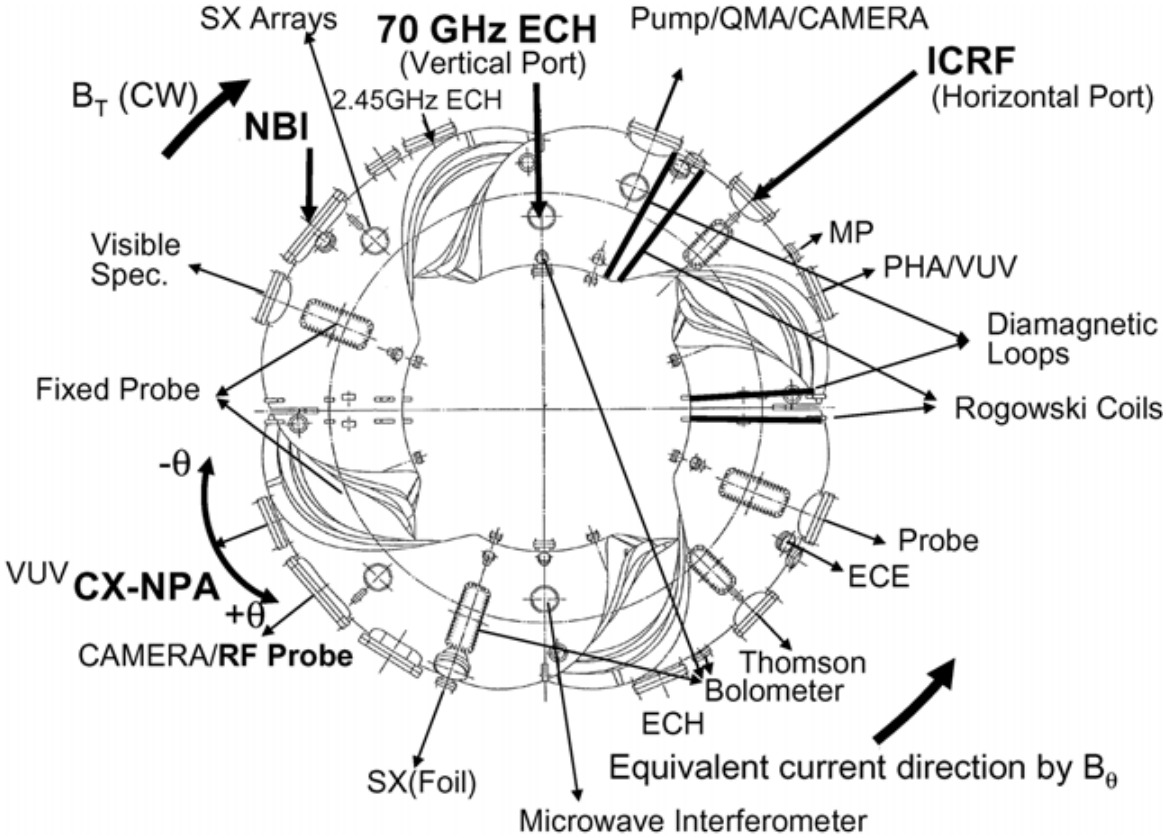
\includegraphics[width=0.7\textwidth]{Images/Locations.jpeg}
  \caption[Heating and diagnostic systems in Heliotron J]{Top-view schematic layout of the heating and diagnostic systems in Heliotron~J. Source: Okada et al.~\cite{Okada2007}.}
  \label{fig:locations}
\end{figure}

\subsection{MHD Instabilities and Alfv\'en Eigenmodes}

\subsubsection{Energetic-Particle-Driven Modes and State of the Art in Heliotron J}
Energetic particles (EPs) generated by NBI form an anisotropic velocity distribution whose free energy resonantly destabilizes shear Alfv\'en waves propagating at the Alfv\'en speed $v_A$ ($\mathrm{m/s}$) in Eq.~(\ref{eqn:alfven}) \cite{Heidbrink2008, Sheikh2023, Adulsiriswad_2024, Varela2015, chen2016introduction}:
\begin{equation}
\label{eqn:alfven}
v_A = \frac{B}{\sqrt{\mu_0 n_i m_i}},
\end{equation}
\noindent where $m_i$ is the ion mass ($\mathrm{kg}$). In three-dimensional heliotrons, periodic magnetic curvature couples poloidal and toroidal harmonics to open frequency gaps in the shear Alfv\'en continuum, sustaining weakly damped Alfv\'en eigenmodes (AEs) \cite{Varela2015, Adulsiriswad_2024}. Mode destabilization requires satisfying the wave--particle resonance condition in Eq.~(\ref{eqn:condition}) \cite{Adulsiriswad_2024}:
\begin{equation}
\label{eqn:condition}
\omega - n\omega_\phi + \ell\omega_\theta = 0,
\end{equation}
\noindent where $\omega$ is the mode angular frequency ($\mathrm{rad/s}$), $n$ is the toroidal mode number, $\omega_\phi$ and $\omega_\theta$ are the EP toroidal transit and poloidal drift frequencies ($\mathrm{rad/s}$), and $\ell$ is an integer bounce/transit harmonic. In flux coordinates $(\theta, \zeta)$, a coherent magnetic perturbation $\tilde{B}$ ($\mathrm{T}$) is decomposed into helical Fourier harmonics via Eq.~(\ref{eqn:periodicity}):
\begin{equation}
\label{eqn:periodicity}    
\tilde{B}(\theta, \zeta) \propto \exp\left[\mathrm{i}(m\theta - n\zeta)\right],
\end{equation}
\noindent where $m$ is the poloidal mode number, $\mathrm{i} = \sqrt{-1}$, and $\theta$ and $\zeta$ are the poloidal and toroidal angles ($\mathrm{rad}$). Continuum gap modes localize near rational flux surfaces where the rotational transform $\iota$ ($\mathrm{rad}$) satisfies Eq.~(\ref{eqn:varela}) \cite{Varela2015}:
\begin{equation}
\label{eqn:varela}
    \frac{\iota}{2\pi} = \frac{n}{m}.
\end{equation}

\noindent Away from exact rational surfaces, the local parallel wavenumber ($\mathrm{m^{-1}}$) is $k_\parallel = (m\iota/(2\pi) - n)/R_0$, where $R_0$ is the major radius ($\mathrm{m}$), while toroidicity-induced harmonic coupling opens the toroidal Alfv\'en eigenmode (TAE) continuum gap centered at $f_{\mathrm{TAE}} = (\iota/2\pi)v_A/(4\pi R_0)$ ($\mathrm{Hz}$) \cite{Heidbrink2008, chen2016introduction, Varela2015}.

In Heliotron~J, experimental observations and Finite Aspect Ratio 3D (FAR3d) gyrofluid and MHD modeling have demonstrated how NBI fast-ion pressure gradients, pitch-angle anisotropy, and three-dimensional magnetic shear govern the excitation of low-$n$ EPMs, BAEs, and global Alfv\'en eigenmodes (GAEs) across the $40\text{--}120~\mathrm{kHz}$ frequency band \cite{Yamamoto_2020, Varela2015, Varela2024, Zhong2024}. Configuration-dependent rotational transform ($\iota/2\pi$) and beam-deposition profiles separate core-localized modes ($m = 1\text{--}4$) from outer-gradient beam-driven BAE/GAE-band instabilities observed near $\rho \approx 0.86\text{--}0.91$ with $m = 6\text{--}8$ \cite{zang2019observation, Varela2023, Zhong2024}. Furthermore, localized ECH and electron cyclotron current drive (ECCD) actively stabilize or shift energetic-particle-driven branches by tailoring core electron temperature and $\iota/2\pi$ \cite{zang2019observation, Varela2023, Adulsiriswad_2024}. Analogous fast-ion Alfv\'enic regimes occur across helical and stellarator experiments, including ECCD stabilization of EPMs and TAEs in the Large Helical Device \cite{Yamamoto_2020, Varela2015}, NBI-driven Alfv\'en eigenmode destabilization controlled by rational-surface topology in the TJ-II stellarator \cite{Varela2017}, and coherent micro-fluctuation characterization via correlation diagnostics in Wendelstein~7-X \cite{KraemerFlecken2024}.

Beyond linear stability, higher-order bispectral and bicoherence techniques reveal nonlinear three-wave coupling that redistributes energy across frequency scales and links macroscopic MHD modes to cross-field transport. Fourier bicoherence measurements have established resonant mode--mode phase locking among Alfv\'enic instabilities in tokamaks \cite{Hou2019} as well as nonlinear coupling between broadband turbulence and coherent modes in toroidal confinement devices \cite{Fujisawa2021}. Specifically in Heliotron~J, bicoherence analyses during the high-confinement mode (H-mode) and across core sawtooth relaxations, in which periodic internal MHD crashes flatten central temperature profiles, demonstrate strong nonlinear coupling between low-frequency MHD modes, edge turbulence, and intermittent confinement degradation \cite{Kin2025, Miyashita2025}. Separating genuine quadratic phase locking from finite-sample variance is thus critical to distinguish coupled daughter harmonics from independent instabilities.

\subsubsection{Theoretical Frequency Scaling Models}
\label{subsubsec:scaling_models}
To identify the physical dispersion of observed modes, instantaneous frequency trajectories are evaluated against seven candidate scaling models \cite{Varela2024}. Ideal shear Alfv\'en dispersion scales inversely with the square root of density as defined in Eq.~(\ref{eqn:shear_alfven}):
\begin{equation}
\label{eqn:shear_alfven}
f_A(t) \propto \frac{v_A(t)}{q R_0} \propto \frac{B}{\sqrt{n_e(t)}},
\end{equation}
\noindent where $f_A(t)$ is the Alfv\'en frequency ($\mathrm{Hz}$), $B$ is the magnetic field magnitude ($\mathrm{T}$), and $q = 2\pi/\iota$ is the safety factor. BAEs and geodesic acoustic modes (GAMs) scale with the ion-acoustic velocity via electron temperature in Eq.~(\ref{eqn:gam}), while compressibility-coupled Alfv\'en--acoustic dispersion follows Eq.~(\ref{eqn:compressibility}):
\begin{equation}
\label{eqn:gam}
f_{\mathrm{BAE}}(t) \propto \sqrt{T_e(t)},
\end{equation}
\begin{equation}
\label{eqn:compressibility}
f(t) \propto \sqrt{\frac{C_1}{n_e(t)} + C_2 T_e(t)},
\end{equation}
\noindent where $f_{\mathrm{BAE}}(t)$ and $f(t)$ are the mode frequencies ($\mathrm{Hz}$) and $C_1, C_2$ are empirical coupling constants. Beam-driven EPMs locked to fast-ion pressure gradients or injection power $P_{\mathrm{NBI}}(t)$ ($\mathrm{W}$) follow Eqs.~(\ref{eqn:epm_density}) and (\ref{eqn:epm_drift}):
\begin{equation}
\label{eqn:epm_density}
f_{\mathrm{EPM}}(t) \propto \sqrt{\frac{P_{\mathrm{NBI}}(t)}{n_e(t)}},
\end{equation}
\begin{equation}
\label{eqn:epm_drift}
f_{\mathrm{EPM}}(t) \propto P_{\mathrm{NBI}}(t),
\end{equation}
\noindent where $f_{\mathrm{EPM}}(t)$ is the energetic-particle-mode frequency ($\mathrm{Hz}$).
Finally, frequency shifts driven by plasma-current-induced rotational transform variations $\Delta\bar{\iota} \propto \Delta I_p$ and finite-$\beta$ diamagnetic equilibrium modifications follow Eq.~(\ref{eqn:shift_macro}):
\begin{equation}
\label{eqn:shift_macro}
f(t) \propto I_p(t), \quad f(t) \propto W_p(t),
\end{equation}
\noindent where $I_p(t)$ is the toroidal plasma current ($\mathrm{A}$) and $W_p(t)$ is the diamagnetic stored energy ($\mathrm{J}$).

\subsection{Signal Processing for MHD Mode Characterization}

\subsubsection{Time-Frequency Analysis}
The spectral bin width $\Delta f$ ($\mathrm{Hz}$) of a short-time Fourier transform (STFT) with window duration $T$ ($\mathrm{s}$) is governed by the Rayleigh frequency resolution limit in Eq.~(\ref{eqn:freq_res}) \cite{proakis2021digital}:
\begin{equation}
\label{eqn:freq_res}
\Delta f = \frac{1}{T}.
\end{equation}
To resolve rapid frequency chirps without fixed-window time--frequency trade-offs \cite{boashash2015time}, the continuous wavelet transform (CWT) employs the complex Morlet mother wavelet $\psi(t)$ in Eq.~(\ref{eqn:morlet}) \cite{addison2016illustrated}:
\begin{equation}
\label{eqn:morlet}
\psi(t) = \pi^{-1/4} \mathrm{e}^{\mathrm{i} \omega_0 t} \mathrm{e}^{-\frac{t^2}{2}},
\end{equation}
\noindent where $t$ is the dimensionless scale-normalized time, $\mathrm{i} = \sqrt{-1}$, and $\omega_0$ is the dimensionless central frequency. Physical modes are isolated from background fluctuations via a dual gate requiring the power spectral density (PSD) $P(f, t)$ ($\mathrm{V^2/Hz}$) to exceed a $3\sigma$ quiescent pre-plasma baseline in Eq.~(\ref{eqn:dominance}) \cite{bendat2010random} while simultaneously exhibiting inter-probe magnitude-squared spatial coherence $\gamma_{xy}^2(f)$ in Eq.~(\ref{eqn:coherence}) \cite{KraemerFlecken2024, Singh2024}:
\begin{equation}
\label{eqn:dominance}
P(f, t) \ge \mu_{\mathrm{noise}}(f) + 3\sigma_{\mathrm{noise}}(f),
\end{equation}
\begin{equation}
\label{eqn:coherence}
\gamma_{xy}^2(f) = \frac{|P_{xy}(f)|^2}{P_{xx}(f) P_{yy}(f)},
\end{equation}
\noindent where $\mu_{\mathrm{noise}}(f)$ and $\sigma_{\mathrm{noise}}(f)$ are the baseline spectral mean and standard deviation ($\mathrm{V^2/Hz}$), and $P_{xy}(f)$, $P_{xx}(f)$, and $P_{yy}(f)$ are the cross- and auto-spectral densities ($\mathrm{V^2/Hz}$). Under independent Gaussian white noise across $N_{\mathrm{seg}}$ non-overlapping segments, the $95\,\%$ coherence significance floor $\gamma_{95}^2$ is given by Eq.~(\ref{eqn:noise_floor}) \cite{carter1973estimation}:
\begin{equation}
\label{eqn:noise_floor}
\gamma_{95}^2 = 1 - (0.05)^{1/(N_{\mathrm{seg}} - 1)}.
\end{equation}
Continuous frequency shifts across heating transitions are tracked without bin-discretization steps via the power-weighted spectral centroid $f_{\mathrm{centroid}}(t)$ ($\mathrm{Hz}$) over $[f_{\min}, f_{\max}]$ in Eq.~(\ref{eqn:spectral_centroid}) \cite{boashash2015time}:
\begin{equation}
\label{eqn:spectral_centroid}
f_{\mathrm{centroid}}(t) = \frac{\sum_{f \in [f_{\min}, f_{\max}]} f \, P(f, t)}{\sum_{f \in [f_{\min}, f_{\max}]} P(f, t)},
\end{equation}
\noindent where $f_{\min}$ and $f_{\max}$ denote the lower and upper spectral band limits ($\mathrm{Hz}$).

\subsubsection{Toroidal Mode Identification}
The toroidal mode number $n$ is determined from the cross-spectral phase difference $\Delta\phi_{ij}^{\mathrm{meas}}$ ($\mathrm{rad}$) between coplanar toroidal probes $x_i, x_j$ ($\mathrm{V}$) at mode frequency $f_0$ ($\mathrm{Hz}$) in Eq.~(\ref{eqn:meas_phase}) \cite{bendat2010random, Smith1971}:
\begin{equation}
\label{eqn:meas_phase}
\Delta\phi_{ij}^{\mathrm{meas}} = \arg\left[P_{x_i x_j}(f_0)\right].
\end{equation}
Comparing against the wrapped theoretical phase shift $\Delta\phi_{ij}^{\mathrm{theo}}(n)$ ($\mathrm{rad}$) for coil toroidal separation $\Delta\varphi_{ij}$ ($\mathrm{rad}$) in Eq.~(\ref{eqn:theo_phase}) \cite{strait2006, Seo2019TheEO}, the best-fit $n$ minimizes the root-mean-square error ($\mathrm{RMSE}(n)$) of the phase fit ($\mathrm{rad}$, reported in degrees in Chapter~\ref{sec:results}) across $N_{\mathrm{pairs}}$ probe pairs in Eq.~(\ref{eqn:rmse}) \cite{schittenhelm1997analysis}:
\begin{equation}
\label{eqn:theo_phase}
\Delta\phi_{ij}^{\mathrm{theo}}(n) = (n \Delta\varphi_{ij} + \pi) \pmod{2\pi} - \pi,
\end{equation}
\begin{equation}
\label{eqn:rmse}
\mathrm{RMSE}(n) = \sqrt{\frac{1}{N_{\mathrm{pairs}}} \sum_{(i,j)} \left(\Delta\phi_{ij}^{\mathrm{meas}} - \Delta\phi_{ij}^{\mathrm{theo}}(n)\right)^2}.
\end{equation}

\subsubsection{Radial Fluctuation Localization and Multi-Coil Cross-Correlation}
\label{subsubsec:theory_ece_radial}
Whereas Mirnov coils measure edge magnetic perturbations $\tilde{B}_\theta$ at the vacuum vessel, internal radial mode localization relies on local electron temperature fluctuations $\tilde{T}_e(\rho, t)$ measured by ECE radiometry in optically thick plasmas \cite{KraemerFlecken2024, luo2020measurement}. For second-harmonic extraordinary-mode (X2) propagation, the emitted microwave frequency $f_{\mathrm{ECE}}$ ($\mathrm{Hz}$) is proportional to the local magnetic field modulus $|B(\rho)|$ ($\mathrm{T}$) in Eq.~(\ref{eqn:ece_resonance}) \cite{chen2016introduction, nagasaki2020heliotron, luo2020measurement}:
\begin{equation}
\label{eqn:ece_resonance}
f_{\mathrm{ECE}} = 2 f_{ce} = \frac{e |B(\rho)|}{\pi m_e},
\end{equation}
\noindent where $f_{ce}$ is the fundamental electron cyclotron frequency ($\mathrm{Hz}$), $e$ is the elementary charge ($\mathrm{C}$), $m_e$ is the electron mass ($\mathrm{kg}$), $\rho = r/a$ is the normalized minor radius, $r$ is the local minor radius ($\mathrm{m}$), and $a = 0.170\,\mathrm{m}$ is the average plasma minor radius. Although the $L=1, M=4$ helical geometry is non-axisymmetric, the ECE antenna at corner-section port \#11.5 (toroidal angle $\phi = \pm 45^\circ$, where toroidal coil A produces a tokamak-like vertical $\mathrm{mod}\text{-}B$ profile) views an equatorial chord along which $|B|$ decreases monotonically from the inboard high-field side to the outboard low-field edge \cite{luo2020measurement, Weir2019}.

Three-dimensional microwave ray-tracing with the Tracing Visualization (\textsc{TRAVIS}) code for the standard configuration (helical-to-vertical coil current ratio $H + V = +89\,\%$, setting the standard vacuum rotational transform $\iota(0)/2\pi \approx 0.56$ at $B_0 \approx 1.25~\mathrm{T}$) parameterizes the equilibrium frequency-to-radius calibration for Heliotron~J port \#11.5 \cite{luo2020measurement, Weir2019} via a first-order exponential decay ($\mathrm{ExpDec1}$, $R^2 = 0.999\ 71$) in Eq.~(\ref{eqn:ece_travis_fit}) and its inverse in Eq.~(\ref{eqn:ece_freq_from_rho}):
\begin{equation}
\label{eqn:ece_travis_fit}
\rho(f) = A_1 \exp\left(-\frac{f}{t_1}\right) + y_0 = 22.290\ 09 \exp\left(-\frac{f}{30.623\ 89}\right) - 2.247\ 43,
\end{equation}
\begin{equation}
\label{eqn:ece_freq_from_rho}
f(\rho) = -t_1 \ln\left(\frac{\rho - y_0}{A_1}\right) = -30.623\ 89 \ln\left(\frac{\rho + 2.247\ 43}{22.290\ 09}\right),
\end{equation}
\noindent where $f$ is the ECE channel frequency ($\mathrm{GHz}$), $y_0 = -2.247\ 43 \pm 0.024\ 14$, $A_1 = 22.290\ 09 \pm 0.314\ 97$, and $t_1 = (30.623\ 89 \pm 0.331\ 98)\,\mathrm{GHz}$, placing the outboard edge ($\rho = 1.00$) at $58.99\,\mathrm{GHz}$, the magnetic axis ($\rho = 0.00$) at $70.26\,\mathrm{GHz}$, and the inboard edge ($\rho = -1.00$) at $88.29\,\mathrm{GHz}$. Because each heterodyne channel integrates over a finite intermediate-frequency (IF) bandwidth $\Delta f_{\mathrm{IF}} \approx 1.0\,\mathrm{GHz}$, each measurement samples a radial shell of width $\Delta \rho$ given by Eq.~(\ref{eqn:ece_radial_res}):
\begin{equation}
\label{eqn:ece_radial_res}
\Delta \rho \approx \left| \frac{\mathrm{d}\rho}{\mathrm{d}f} \right| \Delta f_{\mathrm{IF}} = \frac{A_1}{t_1} \exp\left(-\frac{f}{t_1}\right) \Delta f_{\mathrm{IF}} \approx 0.08\text{--}0.09,
\end{equation}
\noindent corresponding to a physical radial resolution $\Delta r \approx a \Delta \rho \approx (1.4\text{--}1.5)\,\mathrm{cm}$ for $a = 0.170\,\mathrm{m}$, where valid local temperature interpretation requires optically thick core emission ($\tau_{\mathrm{opt}} \gg 1$, $\rho < 0.60$) \cite{luo2020measurement}.

To verify that internal ECE fluctuations couple to the global boundary mode across all 18 Mirnov coils (MP1--MP4 and PMP1--PMP14), the normalized carrier cross-correlation $R_{\mathrm{car}}(\tau)$ evaluates fast phase-coherent coupling within $|\tau| \le 25\,\mu\mathrm{s}$ in Eq.~(\ref{eqn:xcorr_carrier}) \cite{Smith1971, bendat2010random}, while the Hilbert envelope cross-correlation $R_{\mathrm{env}}(\tau)$ captures wave-packet modulation across $|\tau| \le 100\,\mu\mathrm{s}$ in Eq.~(\ref{eqn:xcorr_envelope}) \cite{Fabus2021, boashash2015time}:
\begin{equation}
\label{eqn:xcorr_carrier}
R_{\mathrm{car}}(\tau) = \frac{\langle \tilde{T}_e(t) \tilde{B}_\theta(t+\tau) \rangle}{\sigma_{\tilde{T}} \sigma_{\tilde{B}}},
\end{equation}
\begin{equation}
\label{eqn:xcorr_envelope}
R_{\mathrm{env}}(\tau) = \frac{\langle [A_{\tilde{T}}(t) - \bar{A}_{\tilde{T}}] [A_{\tilde{B}}(t+\tau) - \bar{A}_{\tilde{B}}] \rangle}{\sigma_{A_{\tilde{T}}} \sigma_{A_{\tilde{B}}}},
\end{equation}
\noindent where $\tau$ is the time lag ($\mathrm{s}$), $\sigma_{\tilde{T}}$ and $\sigma_{\tilde{B}}$ are the bandpass-filtered signal standard deviations ($\mathrm{V}$), $\bar{A}_{\tilde{T}}, \bar{A}_{\tilde{B}}$ and $\sigma_{A_{\tilde{T}}}, \sigma_{A_{\tilde{B}}}$ are the temporal means and standard deviations ($\mathrm{V}$) of the Hilbert envelopes $A_{\tilde{T}}(t)$ and $A_{\tilde{B}}(t)$, and $\langle \cdot \rangle$ is the temporal averaging operator. Combined with cross-spectral coherence $\gamma_{\tilde{T}\tilde{B}}^2(f)$ (Eq.~(\ref{eqn:coherence})) against $\gamma_{95}^2$ (Eq.~(\ref{eqn:noise_floor})), these metrics quantify internal-to-external mode coupling. Evaluated between adjacent ECE channels, this dual formalism distinguishes microscopic wave phase progression from macroscopic energy transport: the carrier phase delay derived from the cross-spectral phase $\Delta\phi$ (Eq.~(\ref{eqn:meas_phase})) reflects the local phase velocity $v_{\mathrm{ph},r}$ or stationary radial eigenmode phase structure \cite{Smith1971, Weir2019}. By contrast, the Hilbert envelope lag from $R_{\mathrm{env}}(\tau)$ (Eq.~(\ref{eqn:xcorr_envelope})) tracks macroscopic wavepacket modulation, measuring the radial group velocity $v_{\mathrm{g},r}$ and cross-field energy propagation direction \cite{Fabus2021, boashash2015time}.

\subsection{Signal Conditioning and Correlation Analysis}

\subsubsection{Instantaneous Parameters and Envelope Dynamics}
To extract continuous mode trajectories without phase distortion, magnetic fluctuation signals $x(t)$ ($\mathrm{V}$) are conditioned with a maximally flat group-delay Bessel bandpass filter \cite{zang2019observation}. The complex analytic signal $z(t)$ is constructed via the Hilbert transform $\mathcal{H}\{x(t)\}$ to obtain the instantaneous amplitude envelope $A(t)$ ($\mathrm{V}$), unwrapped phase $\phi(t)$ ($\mathrm{rad}$), and Savitzky--Golay differentiated instantaneous frequency $f(t)$ ($\mathrm{Hz}$) in Eq.~(\ref{eqn:hilbert_inst}) \cite{boashash2015time, Fabus2021}:
\begin{equation}
\label{eqn:hilbert_inst}
z(t) = x(t) + \mathrm{i}\mathcal{H}\{x(t)\} = A(t)\mathrm{e}^{\mathrm{i}\phi(t)}, \qquad f(t) = \frac{1}{2\pi}\frac{\mathrm{d}\phi(t)}{\mathrm{d}t}.
\end{equation}
Active mode bursts are isolated against non-Gaussian background noise and transient spikes using the Gaussian-consistent median absolute deviation (MAD) estimator $\hat{\sigma}_{\mathrm{MAD}}$ ($\mathrm{V}$) in Eq.~(\ref{eqn:mad_sigma}) \cite{RousseeuwCroux1993, james2021statistical}:
\begin{equation}
\label{eqn:mad_sigma}
\hat{\sigma}_{\mathrm{MAD}} = 1.4826\,\mathrm{median}\!\left(\left|x(t) - \mathrm{median}(x)\right|\right).
\end{equation}

\subsubsection{Spatial Harmonic Decomposition and Poloidal Phase}
To resolve the poloidal mode number $m$ across the irregularly spaced PMP1--PMP14 array and suppress spatial aliasing \cite{Klein2008}, the spatial NUDFT is evaluated via Eq.~(\ref{eqn:nudft}) \cite{dutt1993fast}:
\begin{equation}
\label{eqn:nudft}
S_k = \frac{1}{N_{\mathrm{probes}}} \sum_{j=1}^{N_{\mathrm{probes}}} S_j \mathrm{e}^{-\mathrm{i} k \theta_j},
\end{equation}
\noindent where $S_k$ is the spatial spectral amplitude at poloidal wavenumber $k$ ($\mathrm{T/s}$), $N_{\mathrm{probes}}$ is the number of poloidal coils, and $S_j$ ($\mathrm{T/s}$) and $\theta_j$ ($\mathrm{rad}$) are the complex temporal Fourier component and poloidal angle of coil $j$. The cross-spectral poloidal phase $\phi_j$ ($\mathrm{rad}$) relative to reference probe $S_{\mathrm{ref}}$ with phase $\phi_{\mathrm{ref}}$ ($\mathrm{rad}$) is extracted via Eq.~(\ref{eqn:pol_phase}) \cite{Smith1971}, and directional phase clustering around candidate harmonic $m$ is quantified by the Mardia--Jupp circular concentration coefficient $r_{\mathrm{circ}}(m) \in [0, 1]$ in Eq.~(\ref{eqn:r_circ}) \cite{mardia2000directional}:
\begin{equation}
\label{eqn:pol_phase}
\phi_j = \arg\left[\langle S_j(f) S_{\mathrm{ref}}^*(f) \rangle\right] - \phi_{\mathrm{ref}},
\end{equation}
\begin{equation}
\label{eqn:r_circ}
r_{\mathrm{circ}}(m) = \frac{1}{N_{\mathrm{probes}}} \sqrt{\left(\sum_{j=1}^{N_{\mathrm{probes}}} \cos(\phi_j - m\theta_j)\right)^2 + \left(\sum_{j=1}^{N_{\mathrm{probes}}} \sin(\phi_j - m\theta_j)\right)^2}.
\end{equation}
Because the three-dimensional $L=1, M=4$ helical geometry breaks single-harmonic poloidal orthogonality and permits coexisting or coupled poloidal harmonics $(m_1, m_2)$, a multi-branch directional phase-residual extension of circular dispersion statistics \cite{mardia2000directional} assigns each probe to its closest resonant branch via Eq.~(\ref{eqn:dual_branch_phase}) with the dual-branch circular concentration $r_{\mathrm{circ}}(m_1, m_2)$ defined in Eq.~(\ref{eqn:r_circ_dual}):
\begin{equation}
\label{eqn:dual_branch_phase}
\Delta\phi_j(m_1, m_2) = \min_{\mu \in \{m_1, m_2\}} \left| \mathrm{atan2}\left(\sin(\phi_j - \mu \theta_j),\, \cos(\phi_j - \mu \theta_j)\right) \right|,
\end{equation}
\begin{equation}
\label{eqn:r_circ_dual}
r_{\mathrm{circ}}(m_1, m_2) = \frac{1}{N_{\mathrm{probes}}} \sqrt{\left(\sum_{j=1}^{N_{\mathrm{probes}}} \cos\Delta\phi_j(m_1, m_2)\right)^2 + \left(\sum_{j=1}^{N_{\mathrm{probes}}} \sin\Delta\phi_j(m_1, m_2)\right)^2},
\end{equation}
\noindent where values of $r_{\mathrm{circ}}$ approaching unity and small mean absolute phase residuals $\overline{|\Delta\phi|}$ indicate coherent spatial phase alignment across the array \cite{mardia2000directional}.

\subsubsection{Correlation and Statistical Significance}
Dynamic response delays between mode parameters and macroscopic plasma profiles are quantified via the normalized lagged cross-correlation $R_{xy}(\tau)$ at time lag $\tau$ ($\mathrm{s}$) across $N$ samples in Eq.~(\ref{eqn:lagged_corr}) \cite{bendat2010random, Zhong2024}:
\begin{equation}
\label{eqn:lagged_corr}
R_{xy}(\tau) = \frac{1}{N} \sum_{t} \left(\frac{x(t) - \bar{x}}{\sigma_x}\right)\left(\frac{y(t+\tau) - \bar{y}}{\sigma_y}\right),
\end{equation}
\noindent where $\bar{x}, \bar{y}$ and $\sigma_x, \sigma_y$ are the sample means and standard deviations of synchronized time series $x(t)$ and $y(t)$. Because serial autocorrelation in smoothed plasma profiles inflates Type~I error rates, the nominal sample size $N$ is reduced to the effective sample size $N_{\mathrm{eff}}$ via Bartlett's joint-autocorrelation formula in Eq.~(\ref{eqn:neff}) \cite{Afyouni2019, shumway2017time}:
\begin{equation}
\label{eqn:neff}
N_{\mathrm{eff}} = \frac{N}{1 + 2 \sum_{k=1}^{M} \rho_x(k)\rho_y(k)},
\end{equation}
\noindent where $\rho_x(k)$ and $\rho_y(k)$ are the sample autocorrelation function (ACF) values of $x(t)$ and $y(t)$ at lag $k$ up to maximum lag $M$. Hypothesis testing employs the autocorrelation-adjusted $t$-statistic in Eq.~(\ref{eqn:t_stat}) \cite{shumway2017time} and first-order partial correlation $r_{xy \cdot z}$ in Eq.~(\ref{eqn:partial_corr}) to control for shared step-function artifacts $z$ \cite{james2021statistical}:
\begin{equation}
\label{eqn:t_stat}
t = r \sqrt{\frac{N_{\mathrm{eff}} - 2 - n_{\mathrm{control}}}{1 - r^2}},
\end{equation}
\begin{equation}
\label{eqn:partial_corr}
r_{xy \cdot z} = \frac{r_{xy} - r_{xz}r_{yz}}{\sqrt{(1 - r_{xz}^2)(1 - r_{yz}^2)}},
\end{equation}
\noindent where $r, r_{xy}, r_{xz}, r_{yz}$ are pairwise Pearson correlation coefficients and $n_{\mathrm{control}}$ is the number of control variables. Family-wise error across $m$ simultaneous tests is controlled via the Bonferroni threshold $\alpha_{\mathrm{adj}}$ in Eq.~(\ref{eq:bonferroni}) \cite{dunn1961multiple} alongside Benjamini--Hochberg false discovery rate (FDR-BH) adjustments \cite{Benjamini1995}:
\begin{equation}
\label{eq:bonferroni}
\alpha_{\mathrm{adj}} = \frac{\alpha}{m},
\end{equation}
\noindent where $m$ is the number of simultaneous hypothesis tests and $\alpha$ is the nominal significance level.

\subsection{Higher-Order Spectral Analysis for Nonlinear Wave Coupling}

\subsubsection{Bicoherence and Coupling Domains}
Quadratic nonlinear three-wave coupling is quantified via the auto-bispectrum $B(f_1, f_2)$ ($\mathrm{V^3/Hz^3}$) in Eq.~(\ref{eqn:bispectrum}) and the normalized squared auto-bicoherence $b^2(f_1, f_2) \in [0, 1]$ in Eq.~(\ref{eqn:bicoherence}) \cite{proakis2021digital, Hou2019, Fujisawa2021}:
\begin{equation}
\label{eqn:bispectrum}
B(f_1, f_2) = \langle X(f_1) X(f_2) X^*(f_1 \pm f_2) \rangle,
\end{equation}
\begin{equation}
\label{eqn:bicoherence}
b^2(f_1, f_2) = \frac{|\langle X(f_1) X(f_2) X^*(f_1 \pm f_2) \rangle|^2}{\langle |X(f_1) X(f_2)|^2 \rangle \langle |X(f_1 \pm f_2)|^2 \rangle},
\end{equation}
\noindent where $X(f)$ is the segmented complex Fourier spectrum ($\mathrm{V/Hz}$) at interacting frequencies $f_1, f_2$ ($\mathrm{Hz}$), $\langle \cdot \rangle$ is the expectation across $N_{\mathrm{ensemble}}$ segments, and $*$ denotes complex conjugation. Under a Gaussian null hypothesis, the significance threshold $b^2_\alpha$ at level $\alpha$ is approximated by Eq.~(\ref{eqn:b2_stat}) \cite{Hou2019, Fujisawa2021, HinichWolinsky2005}:
\begin{equation}
\label{eqn:b2_stat}
b^2_\alpha = -\frac{\ln(\alpha)}{N_{\mathrm{ensemble}}}.
\end{equation}
To eliminate bispectral permutation redundancies while maintaining positive physical frequencies ($f_1 > 0, f_2 > 0$), resonant triads are partitioned into sum-coupling (up-conversion) and difference-coupling (parametric decay / difference interaction) domains in Eqs.~(\ref{eqn:sum_domain}) and (\ref{eqn:diff_domain}):
\begin{equation}
\label{eqn:sum_domain}
f_3 = f_1 + f_2 \quad (f_1 > 0,\; f_2 > 0),
\end{equation}
\begin{equation}
\label{eqn:diff_domain}
f_3 = |f_1 - f_2| \quad (\text{or } f_1 - f_2 = f_3 \text{ with } f_1 > f_2 > 0),
\end{equation}
\noindent where $f_3$ is the coupled frequency ($\mathrm{Hz}$) bounded by the Nyquist limit; in the general bispectral notation $B(f_1, f_2) = \langle X(f_1) X(f_2) X^*(f_1 + f_2) \rangle$, a positive-frequency difference triad $f_a - f_b = f_c$ corresponds to setting $f_2 = -f_b$ via Hermitian symmetry $X(-f_b) = X^*(f_b)$.

\subsubsection{Bias Scaling, Convergence Extrapolation, and Empirical Benchmarking}
Because finite-sample bicoherence estimators carry positive bias ($\mathrm{E}[\hat{b}^2] \approx 1/N_{\mathrm{ensemble}}$) \cite{HinichWolinsky2005}, candidate transition shifts and triads in heated windows \cite{Kin2025, Miyashita2025} are benchmarked against $N_{\mathrm{null}}$ null realizations via the Davison--Hinkley empirical $p$-value ($p_{\mathrm{emp}}$) in Eq.~(\ref{eqn:empirical_p}) \cite{DavisonHinkley1997, james2021statistical}:
\begin{equation}
\label{eqn:empirical_p}
p_{\mathrm{emp}} = \frac{k + 1}{N_{\mathrm{null}} + 1},
\end{equation}
\noindent where $k$ is the count of null realizations equaling or exceeding the observed statistic. To separate genuine quadratic phase locking from $O(1/K)$ finite-sample bias across $K$ averaged segments, the sub-ensemble convergence trajectory $b^2(K)$ is regressed linearly against $1/K$ and extrapolated to the infinite-ensemble limit ($1/K \to 0$) via Eq.~(\ref{eqn:b2_convergence}) \cite{KimPowers1979, HinichWolinsky2005}:
\begin{equation}
\label{eqn:b2_convergence}
b^2(K) = b_0 + \frac{C}{K},
\end{equation}
\noindent where $b_0 = b^2_\infty$ is the asymptotic squared bicoherence intercept and $C$ is the finite-sample bias slope. Chronological non-stationarities are suppressed by averaging $N_{\mathrm{sub}}$ random sub-ensembles sampled without replacement over $K \in [K_{\mathrm{min}}, 0.9\,N_{\mathrm{seg}}]$ (where $K_{\mathrm{min}}$ is the minimum averaged sub-ensemble size and $N_{\mathrm{seg}}$ is the total segment count), extracting $95\,\%$ confidence bounds $[q_{2.5}, q_{97.5}]$ defined as the $2.5\text{th}$ and $97.5\text{th}$ empirical percentiles of the sub-ensemble intercept distribution. Finally, $b_0$ is calibrated against $N_{\mathrm{null}}$ Fourier phase-randomized surrogates ($\phi_k \sim \mathcal{U}[0, 2\pi)$) preserving the exact sample PSD under $H_0: b^2_{\mathrm{pop}} = 0$, yielding the surrogate significance $p_{\mathrm{surr}}$ via Eq.~(\ref{eqn:empirical_p}).
\newpage

\section{Methodology}

Within Heliotron~J's flexible $L=1, M=4$ helical configuration, coil currents, heating schedules, and diagnostic availability varied across campaigns, altering energetic-particle confinement and MHD stability. Screening matched configurations for complete 18-coil Mirnov and 16-channel ECE coverage, sustained $\mathrm{NBI}+\mathrm{ECH}$ heating ($>30~\mathrm{ms}$), zero analog-to-digital converter (ADC) rail saturation or switching spikes, and clean spectrograms yielded primary shot \#88653 and unpooled replicate \#88654 (Annex~\ref{annex:data}). Operationally, Objective~1 mapped Mirnov decomposition, radial ECE localization (Section~\ref{subsubsec:method_ece_radial}), and ECH switch-off tracking (Section~\ref{subsubsec:method_ech_off}) to mode structure and transition dynamics; Objective~2 tested heating synchronization and dispersion scalings via autocorrelation-adjusted partial correlations and LPF ECE $T_e$ proxies (Section~\ref{subsubsec:method_scaling}); and Objective~3 isolated nonlinear coupling via surrogate-calibrated auto-bicoherence (Figure~\ref{fig:methodology_pipeline}, Appendix~\ref{appendix:github}).

Workflows ran in 64-bit Python~3.12.4 by the Python Software Foundation on the 64-bit ARM (ARM64) architecture using \texttt{NumPy} 1.26.4, \texttt{SciPy} 1.13.1---via \texttt{scipy.\allowbreak signal} and \texttt{scipy.\allowbreak stats} for spectral estimation, Bessel and Butterworth second-order section (SOS) infinite impulse response (IIR) filters, Savitzky--Golay differentiation, Hilbert transforms, and significance testing---and \texttt{Matplotlib}~3.9.2, exporting peak catalogs in JavaScript Object Notation (JSON) format. Raw Experimental Data Format (EDF, \texttt{.edf}) records were parsed with \texttt{turnelib} and \texttt{PyEDFlib} 0.1.38 atop \texttt{jpack}~2025 v1.0 (\texttt{libana\_\allowbreak signal}, \texttt{hjlib}, \texttt{matplotlibutil}; IAE, Kyoto University), with ECE radial mapping via the \textsc{TRAVIS} 3D ray-tracing code (Max Planck Institute for Plasma Physics, Greifswald; Table~\ref{tab:work_schedule}).

\begin{figure}[H]
  \centering
  \begin{tikzpicture}[
    font=\sffamily,
    >=Stealth,
    node distance=0.35cm and 0.34cm,
    pbox/.style={
      rectangle, rounded corners=3.5pt, draw=#1, fill=white, line width=0.8pt,
      align=center, inner xsep=4pt, inner ysep=3.5pt, font=\footnotesize,
      minimum height=1.06cm
    },
    rbox/.style={
      rectangle, rounded corners=3.5pt, draw=red!70!black, fill=red!6!white, line width=0.9pt,
      align=center, inner xsep=4pt, inner ysep=3.5pt, font=\footnotesize,
      minimum height=1.06cm
    },
    panel/.style={
      rounded corners=5pt, draw=#1!65!black, fill=#1!5!white, line width=0.7pt,
      inner xsep=6pt, inner ysep=4.5pt
    },
    arr/.style={->, line width=0.85pt, draw=#1, rounded corners=3pt}
  ]
  % --- Objective 1: 2 rows x 3 cols (aligned identically with Obj 2 & 3 right edge) ---
  \node[pbox=blue!65!black, text width=4.48cm] (o1_1) at (0,0)
    {\textbf{\small Mirnov Signals}\\[2pt] Coils \texttt{MP1}, \texttt{MP3}, \texttt{MP4}};
  \node[pbox=blue!65!black, text width=4.48cm, right=0.50cm of o1_1] (o1_2)
    {\textbf{\small Time--Frequency Maps}\\[2pt] STFT \& CWT decompositions};
  \node[rbox, text width=4.48cm, right=0.50cm of o1_2] (o1_3)
    {\textbf{\small Dual-Criterion Gate}\\[2pt] $P \ge \mu + 3\sigma$ and $\gamma^2 > 0.7$};

  \node[pbox=blue!65!black, text width=4.48cm, below=0.40cm of o1_1] (o1_4)
    {\textbf{\small Peak Selection}\\[2pt] Mode tracking \& JSON export};
  \node[pbox=blue!65!black, text width=4.48cm, right=0.50cm of o1_4] (o1_5)
    {\textbf{\small Modal Extraction}\\[2pt] NUDFT spatial mode extraction};
  \node[pbox=blue!65!black, text width=4.48cm, right=0.50cm of o1_5] (o1_6)
    {\textbf{\small ECE Localization}\\[2pt] 16-channel radial \& ECH-off};

  \node[anchor=south west, font=\footnotesize\bfseries\sffamily, text=blue!65!black] (o1_lbl)
    at ([yshift=2pt]o1_1.north west) {Objective 1: Spectral \& Spatial Characterization};

  % --- Root node centered cleanly above Objective 1 ---
  \node[pbox=gray!55!black, fill=gray!6!white, text width=7.6cm, minimum height=0.84cm,
        above=0.50cm of o1_2] (root)
    {\textbf{\small Shot Selection}\\[1pt] Diagnostic availability \& flat-top screening (\#88653, \#88654)};

  % --- Objective 2: 5 cols ---
  \node[pbox=teal!75!black, text width=2.55cm, below=0.70cm of o1_4.south west, anchor=north west] (o2_1)
    {\textbf{\small Diagnostic}\\\textbf{\small Data}\\[2pt] Heating, ECE \&\\[-1pt]$n_e$ profiles};
  \node[pbox=teal!75!black, text width=2.55cm, right=0.28cm of o2_1] (o2_2)
    {\textbf{\small Signal}\\\textbf{\small Envelope}\\[2pt] Bessel filter\\[-1pt]+ Hilbert};
  \node[rbox, text width=2.55cm, right=0.28cm of o2_2] (o2_3)
    {\textbf{\small Burst}\\\textbf{\small Detection}\\[2pt] MAD threshold\\[-1pt]+ close};
  \node[pbox=teal!75!black, text width=2.55cm, right=0.28cm of o2_3] (o2_4)
    {\textbf{\small Correlation}\\\textbf{\small Suite}\\[2pt] Lagged, $N_{\mathrm{eff}}$\\[-1pt]\& partial};
  \node[pbox=teal!75!black, text width=2.55cm, right=0.28cm of o2_4] (o2_5)
    {\textbf{\small Scaling}\\\textbf{\small Models}\\[2pt] LPF ECE $T_e$\\[-1pt]\& BAE};

  \node[anchor=south west, font=\footnotesize\bfseries\sffamily, text=teal!75!black] (o2_lbl)
    at ([yshift=2pt]o2_1.north west) {Objective 2: Heating Correlation};

  % --- Objective 3: 5 cols ---
  \node[pbox=orange!70!black, text width=2.55cm, below=0.70cm of o2_1] (o3_1)
    {\textbf{\small Stored}\\\textbf{\small Energy}\\[2pt] Diamagnetic\\[-1pt]signal $W_p$};
  \node[pbox=orange!70!black, text width=2.55cm, right=0.28cm of o3_1] (o3_2)
    {\textbf{\small Burst}\\\textbf{\small Window}\\[2pt] Hysteresis\\[-1pt]detection};
  \node[pbox=orange!70!black, text width=2.55cm, right=0.28cm of o3_2] (o3_3)
    {\textbf{\small Bispectrum}\\[2pt] Bicoherence\\[-1pt]coupling matrix};
  \node[rbox, text width=2.55cm, right=0.28cm of o3_3] (o3_4)
    {\textbf{\small Dual}\\\textbf{\small Validation}\\[2pt] Reproducibility\\[-1pt]+ cross-diag.};
  \node[pbox=orange!70!black, text width=2.55cm, right=0.28cm of o3_4] (o3_5)
    {\textbf{\small Asymptotic}\\\textbf{\small Validation}\\[2pt] $1/K$ conv.\ \&\\[-1pt]500 surrogates};

  \node[anchor=south west, font=\footnotesize\bfseries\sffamily, text=orange!70!black] (o3_lbl)
    at ([yshift=2pt]o3_1.north west) {Objective 3: Nonlinear Coupling};

  % --- Background panels ---
  \begin{scope}[on background layer]
    \node[panel=blue, fit=(o1_1)(o1_3)(o1_4)(o1_6)(o1_lbl)] (p1) {};
    \node[panel=teal, fit=(o2_1)(o2_5)(o2_lbl)] (p2) {};
    \node[panel=orange, fit=(o3_1)(o3_5)(o3_lbl)] (p3) {};
  \end{scope}

  % --- Spine from Shot Selection to each Objective panel ---
  \coordinate (trunk) at ([xshift=-0.42cm]p1.west);
  \draw[arr=blue!65!black] (root.west) -| (trunk |- p1.west) -- (p1.west);
  \draw[arr=teal!75!black] (trunk |- p1.west) -- (trunk |- p2.west) -- (p2.west);
  \draw[arr=orange!70!black] (trunk |- p2.west) -- (trunk |- p3.west) -- (p3.west);

  % --- Intra-panel arrows ---
  \draw[arr=blue!65!black] (o1_1) -- (o1_2);
  \draw[arr=blue!65!black] (o1_2) -- (o1_3);
  \draw[arr=blue!65!black] (o1_3.south) -- ++(0,-0.26) -| (o1_4.north);
  \draw[arr=blue!65!black] (o1_4) -- (o1_5);
  \draw[arr=blue!65!black] (o1_5) -- (o1_6);

  \draw[arr=teal!75!black] (o2_1) -- (o2_2);
  \draw[arr=teal!75!black] (o2_2) -- (o2_3);
  \draw[arr=teal!75!black] (o2_3) -- (o2_4);
  \draw[arr=teal!75!black] (o2_4) -- (o2_5);

  \draw[arr=orange!70!black] (o3_1) -- (o3_2);
  \draw[arr=orange!70!black] (o3_2) -- (o3_3);
  \draw[arr=orange!70!black] (o3_3) -- (o3_4);
  \draw[arr=orange!70!black] (o3_4) -- (o3_5);
  \end{tikzpicture}
  \caption[Methodology pipeline]{Methodology pipeline. Source: Own elaboration.}
  \label{fig:methodology_pipeline}
\end{figure}

\begin{table}[H]
\centering
\scriptsize
\setlength{\tabcolsep}{3pt}
\renewcommand{\arraystretch}{0.82}
\caption[Execution schedule of the Final Graduation Project activities]{Execution schedule of the Final Graduation Project activities. Source: Own elaboration.}
\label{tab:work_schedule}
\begin{tabularx}{\textwidth}{@{}l >{\raggedright\arraybackslash}X >{\raggedright\arraybackslash}p{3.0cm} c c@{}}
\toprule
Stage & Activity Description & Deliverable & Objective & Period \\
\midrule
1 & Literature review, shot screening, and \texttt{jpack} setup & Curated shot list and software stack & General & Jul--Aug 2026 \\
2 & STFT/CWT, $3\sigma$/$\gamma^2$ gate, NUDFT ($m,n$), and 16-ECE $\times$ 18-Mirnov localization & Mode catalog and spatial maps & Objective~1 & Aug--Oct 2026 \\
3 & Bessel/Hilbert, MAD bursts, partial $r$ ($N_{\mathrm{eff}}$), and LPF ECE $T_e$/BAE scalings & Heating correlation and scaling tables & Objective~2 & Sep--Oct 2026 \\
4 & Corrected auto-bicoherence, 33 reference windows, and $1/K$ convergence surrogates & Asymptotic triad validation figures & Objective~3 & Oct--Nov 2026 \\
5 & Cross-objective synthesis, literature benchmarking, statistical audit, and thesis writing & Final thesis and open-source code & All & Oct--Nov 2026 \\
\bottomrule
\end{tabularx}
\end{table}

\subsection{First Specific Objective}
Objective~1 characterized MHD spectral evolution, spatial mode structure, radial position, and ECH switch-off response in Heliotron~J \cite{nagasaki2020heliotron, Yamamoto_2020} using an automated dual-criterion coherence gate.

\subsubsection{Data Acquisition and Preprocessing}
Discharges used a deuterium bulk plasma ($\mathrm{D}_2$, $m_i = 2m_p$) heated by hydrogen ($\mathrm{H}^0$) neutral beams, yielding mixed $\mathrm{D}^+/\mathrm{H}^+$ populations with $m_{\mathrm{eff}} \in [1.0, 2.0]\,m_p$ \cite{Yamamoto_2020, nagasaki2020heliotron}. Diagnostics were retrieved from \texttt{.edf} archives via \texttt{turnelib} (\texttt{jpack}, Annex~\ref{annex:library}) on custom IAE, Kyoto University Computer Automated Measurement and Control (CAMAC) and Peripheral Component Interconnect (PCI) eXtensions for Instrumentation (PXI) transient digitizers ($\pm 5.0~\mathrm{V}$ bipolar range) \cite{nagasaki2020heliotron, zang2019observation}. Custom IAE Mirnov coils (\texttt{MP1}--\texttt{MP4}, gain $G = 200$, $NA = 30 \times 15 \times 10^{-6}~\mathrm{m^2}$; \texttt{PMP1}--\texttt{PMP14}, $G = 2.0$, $NA = 4.5 \times 10^{-3}~\mathrm{m^2}$) used 12-bit \texttt{530-1} modules at $f_s = 1.0~\mathrm{MHz}$ ($262\,144$ samples), alongside 16-bit \texttt{E500-2} $\mathrm{H}_\alpha$ monitors (\texttt{HAFAST3.5}--\texttt{15.5}) and 16-bit \texttt{E501-3} radiometry at $1.0~\mathrm{MHz}$ \cite{nagasaki2020heliotron, zang2019observation}.

Equilibrium signals used an IAE 16-bit \texttt{40088-1} digitizer at $100~\mathrm{kHz}$ ($131\,072$ samples) for custom diamagnetic loops (\texttt{DIA135-DEF1/2}, $W_p$, $G = 50.0$) and Rogowski coil (\texttt{ROG15}, $I_p$, $G = 500.0$), a 14-bit \texttt{E700-1} module at $10.0~\mathrm{MHz}$ ($4 \times 10^6$ samples) for the IAE $2~\mathrm{mm}$ ($140~\mathrm{GHz}$) interferometer (\texttt{MICRO-1/2}, $n_e$, $G = 1.0$), and 12-bit \texttt{5909-2} channels at $5.0~\mathrm{kHz}$ for the Toshiba $70~\mathrm{GHz}$, $0.4~\mathrm{MW}$ X2 gyrotron (\texttt{ECHRG500}, $-1000~\mathrm{kW/V}$) and IAE $30~\mathrm{keV}$, $0.7~\mathrm{MW}$ NBI monitors (Beam Lines~1 and~2 [\texttt{BL1}/\texttt{BL2}]; \texttt{NBIS9I}/\texttt{NBIS10I} [plotted as \texttt{NBIS9}/\texttt{NBIS10}], $100~\mathrm{A/V}$) \cite{Yamamoto_2020, nagasaki2020heliotron}. Internal $T_e$ oscillations were measured at port \#11.5 by the IAE 16-channel X2 ECE radiometer ($57.5\text{--}72.5~\mathrm{GHz}$, $56$/$64~\mathrm{GHz}$ local oscillators (LOs), $1.0~\mathrm{GHz}$ IF stages) \cite{luo2020measurement, Weir2019}. Following International System of Units (SI) conventions, plots reported quantities in standard decimal prefixes ($\mathrm{ms}$, $\mathrm{kHz}$, $\mathrm{GHz}$, $\mathrm{kA}$, $\mathrm{kJ}$, $\mathrm{kW}$) with volts ($\mathrm{V}$) or arbitrary units ($\mathrm{a.u.}$). Coplanar probes \texttt{MP1}, \texttt{MP3}, and \texttt{MP4} provided 1D toroidal phases, excluding off-midplane \texttt{MP2} ($\theta \neq 0^\circ$) to avoid poloidal mixing \cite{Seo2019TheEO, schittenhelm1997analysis}, whereas all 18 coils entered radial ECE cross-correlation.

\subsubsection{Time-Frequency Analysis}
Stationary and transient \texttt{MP1} dynamics used an STFT PSD spectrogram (\texttt{libana\_signal}, Hann window, Eq.~(\ref{eqn:freq_res})) \cite{proakis2021digital} at $N_{\mathrm{fft}} = 2000$ ($500~\mathrm{Hz}$ resolution) for tracking, $256/1024$ samples ($3.9/0.977~\mathrm{kHz}$) across ECH off, and $512$ samples ($1.953~\mathrm{kHz}$) for bicoherence, paired with a complex Morlet CWT ($\omega_0 = 6$, Eq.~(\ref{eqn:morlet}), $\pm 5\sigma$ support, $150$ bins over $10\text{--}150~\mathrm{kHz}$) \cite{boashash2015time, addison2016illustrated}. Secondary and primary modes used $40\text{--}80~\mathrm{kHz}$ and $80\text{--}120~\mathrm{kHz}$ passbands ($80\text{--}100~\mathrm{kHz}$ for steady ECE localization; $30\text{--}55~\mathrm{kHz}$ and $75\text{--}105~\mathrm{kHz}$ across ECH switch-off).

\subsubsection{Dual-Criterion Mode Identification}
Physical modes within $15\text{--}100~\mathrm{kHz}$ required both $4~\mathrm{ms}$ rolling power exceeding a $3\sigma$ baseline (Eq.~(\ref{eqn:dominance}), calibrated on $150~\mathrm{ms} \text{--}175~\mathrm{ms}$, slightly overlapping ECH turn-on at $171.2~\mathrm{ms}$) for $\ge 2~\mathrm{ms}$---enforcing $99.7\,\%$ Gaussian false-alarm rejection over $\ge 80$ cycles \cite{bendat2010random}---and Welch coherence $\gamma^2 > 0.7$ ($100$ ensembles, Eq.~(\ref{eqn:coherence}), $>70\,\%$ phase-coherent variance) on at least one of \texttt{MP1}--\texttt{MP3}, \texttt{MP1}--\texttt{MP4}, or \texttt{MP3}--\texttt{MP4} \cite{KraemerFlecken2024, Singh2024}, with confirmed peaks saved as JSON.

\subsubsection{Poloidal (\texorpdfstring{$m$}{m}) and Toroidal (\texorpdfstring{$n$}{n}) Mode Decomposition}
After $\mathrm{T/s}$ calibration and polarity inversion of \texttt{PMP1}--\texttt{PMP4} (Appendix~\ref{appendix:poloidalm}), poloidal numbers $m$ were extracted from \texttt{PMP1}--\texttt{PMP14} via spatial NUDFT (Eqs.~(\ref{eqn:nudft})--(\ref{eqn:pol_phase})) \cite{dutt1993fast, Klein2008} over $m = \pm 6$ (expanding to $\pm 20$ if boundary-pinned) with a synthetic alias-free self-test. Because single-mode $40\text{--}80~\mathrm{kHz}$ fits left large equatorial residuals, an exhaustive two-mode search scanned all $\binom{41}{2} = 820$ pairs $(m_1, m_2) \in [-20, +20]^2$ using closest-branch phase assignment (Eq.~(\ref{eqn:dual_branch_phase})) and $r_{\mathrm{circ}}(m_1, m_2)$ (Eq.~(\ref{eqn:r_circ_dual})). Plots used an automated $8.0~\mathrm{ms}$ minimal-$|\mathrm{d}f/\mathrm{d}t|$ sub-window in $259.1\text{--}275.0~\mathrm{ms}$ ($50~\%$ slope tolerance), plus fixed $\mathrm{ECH}+\mathrm{NBI}$ ($259.1\text{--}291.3~\mathrm{ms}$), $\mathrm{NBI}$-only ($291.3\text{--}300.0~\mathrm{ms}$), and post-transition $87~\mathrm{kHz}$ slices ($291.4\text{--}291.8~\mathrm{ms}$ in \#88653; $292.0\text{--}293.0~\mathrm{ms}$ in \#88654). Fits with $r_{\mathrm{circ}} \ge 0.70$ and mean absolute error $\le 45^\circ$ were \emph{supported} (else \emph{unresolved}), while toroidal $n$ from \texttt{MP1}, \texttt{MP3}, and \texttt{MP4} (Eqs.~(\ref{eqn:meas_phase})--(\ref{eqn:rmse})) remained defined modulo~$4$.

\subsubsection{Radial Fluctuation Profiling and Multi-Coil Cross-Correlation}
\label{subsubsec:method_ece_radial}
\begin{sloppypar}
The 16 ECE channels (\texttt{ECE1FAST}--\allowbreak\texttt{ECE16FAST}, $1~\mathrm{GHz}$ spacing) \cite{luo2020measurement, Weir2019} were mapped to $\rho = r/a$ via Eq.~(\ref{eqn:ece_travis_fit}) ($\Delta \rho \approx 0.08\text{--}0.09$, Eq.~(\ref{eqn:ece_radial_res})) and profiled across $\mathrm{ECH}+\mathrm{NBI}$ ($259.1\text{--}291.3~\mathrm{ms}$), $\mathrm{NBI}$-only ($291.3\text{--}300.0~\mathrm{ms}$), its step-free tail ($294.2\text{--}300.0~\mathrm{ms}$), and $259.1\text{--}275.0~\mathrm{ms}$ in $40\text{--}80~\mathrm{kHz}$ and $80\text{--}100~\mathrm{kHz}$. Localization required: (i)~bandpass root-mean-square (RMS) $\tilde{T}_e > 10\times$ the $150\text{--}175~\mathrm{ms}$ pre-plasma floor; (ii)~adjacent-channel $\gamma^2 > 0.70$; and (iii)~all $16 \times 18$ ECE--Mirnov cross-correlations via carrier $|r_{\mathrm{car}}(\tau)|$ ($|\tau| \le 25~\mu\mathrm{s}$, Eq.~(\ref{eqn:xcorr_carrier})), envelope $|r_{\mathrm{env}}(\tau)|$ ($|\tau| \le 100~\mu\mathrm{s}$, Eq.~(\ref{eqn:xcorr_envelope})), and $\gamma^2(f)$ ($N_{\mathrm{fft}} = 1024, 2048$, $50~\%$ overlap) above $\gamma_{95}^2$ (Eq.~(\ref{eqn:noise_floor})), using $\Delta\phi_{xy}(f)$ and lagged correlations for adjacent propagation.
\end{sloppypar}

\subsubsection{Response to ECH Switch-Off}
\label{subsubsec:method_ech_off}
Transition dynamics were evaluated on \#88653 with \#88654 as an unpooled same-sign check across one transition per shot ($N=1$; ECH on $171.2~\mathrm{ms}$, NBI on $222.4~\mathrm{ms}$, ECH off $291.32~\mathrm{ms}$ at \texttt{ECHRG500} half-drop with reference $t_0 = 291.20~\mathrm{ms}$, NBI off $300.4~\mathrm{ms}$). Phase-resolved \texttt{MP1} RMS and \texttt{MP1}--\texttt{MP3} coherence tracked persistence, while piecewise linear fits over $2$ and $5~\mathrm{ms}$ windows around $t_0$ yielded $\Delta(\mathrm{d}W_p/\mathrm{d}t)$ and block-bootstrap intervals inside NBI sustainment. Spectral shifts ($30\text{--}55~\mathrm{kHz}$, $75\text{--}105~\mathrm{kHz}$) compared $[t_0-2.0,\,t_0]~\mathrm{ms}$ vs.\ $[t_0+1.5,\,t_0+3.5]~\mathrm{ms}$ centroids (Eq.~(\ref{eqn:spectral_centroid})) and peak bins, null-calibrated across $261.0\text{--}287.5~\mathrm{ms}$ via $54$ sliding ($0.5~\mathrm{ms}$ step) and $5$ disjoint windows ($p \ge 0.167$, Eq.~(\ref{eqn:empirical_p})) plus $500$ block permutations, alongside $f \propto n_e^{-\gamma}$ fits $(262\text{--}290$, $270\text{--}290$, $275\text{--}291.2)~\mathrm{ms}$ tested at $290.2$ and $293.7~\mathrm{ms}$.

\subsection{Second Specific Objective}
Objective~2 quantified EPM--heating synchronization by correlating conditioned magnetic envelopes and instantaneous frequencies with macroscopic proxies \cite{Adulsiriswad_2024, Varela2023, Zhong2024}.

\subsubsection{Signal Conditioning and Active Burst Detection}
Heating, ECE, and $n_e$ traces were linearly interpolated onto the $1~\mathrm{MHz}$ Mirnov grid (Figure~\ref{fig:methodology2}). Magnetic signals were filtered (4th-order Bessel bandpass) and Hilbert-transformed for envelope $A(t)$ and unwrapped phase $\phi(t)$ (Eq.~(\ref{eqn:hilbert_inst})) \cite{zang2019observation, Fabus2021}, with $f(t)$ via $525$-sample ($0.525~\mathrm{ms}$) Savitzky--Golay differentiation chosen via bandwidth sweeps to suppress phase-derivative noise while preserving millisecond chirps. Active bursts selected the longest contiguous interval ($> 10.0~\mathrm{ms}$, gaps $\le 3.0~\mathrm{ms}$ bridged) above $\mathrm{median} + 6.0\,\hat{\sigma}_{\mathrm{MAD}}$ (Eq.~(\ref{eqn:mad_sigma})) prior to $100\times$ cascaded IIR decimation \cite{boashash2015time, Fabus2021}.

\begin{figure}[H]
  \centering
  \begin{tikzpicture}[
    font=\sffamily,
    >=Stealth,
    tbox/.style={
      rectangle, rounded corners=3.5pt, draw=#1, fill=white, line width=0.85pt,
      align=center, inner xsep=3.5pt, inner ysep=5pt, font=\footnotesize,
      minimum height=1.55cm
    },
    arr/.style={->, line width=0.9pt, draw=teal!75!black, rounded corners=3pt}
  ]
  % 2x2 Objective 2 conditioning grid in center
  \node[tbox=teal!75!black, text width=4.05cm] (c1)
    {\textbf{\small Bessel Bandpass}\\[2pt] Maximally flat delay\\(zero phase distortion)};
  \node[tbox=teal!75!black, text width=4.05cm, right=0.44cm of c1] (c2)
    {\textbf{\small Analytic Signal}\\[2pt] Hilbert transform $\mathcal{H}[\cdot]$\\Envelope $A(t)$ \& phase $\phi(t)$};
  \node[tbox=teal!75!black, text width=4.05cm, anchor=north] (c3) at ([yshift=-0.65cm]c1.south |- c2.south)
    {\textbf{\small Savitzky--Golay}\\[2pt] 525-sample polynomial\\Preserves sweep dynamics};
  \node[tbox=teal!75!black, text width=4.05cm, right=0.44cm of c3] (c4)
    {\textbf{\small Decimation ($\times 100$)}\\[2pt] Multi-stage anti-alias\\Ensures IIR stability};

  \node[anchor=south west, font=\footnotesize\bfseries\sffamily, text=teal!75!black, align=left] (lbl2)
    at ([yshift=2pt]c1.north west) {Objective 2: Signal Conditioning \&\\Dynamic Parameter Extraction};

  \begin{scope}[on background layer]
    \node[rounded corners=5pt, draw=teal!60!black, fill=teal!5!white, line width=0.7pt,
          inner xsep=4pt, inner ysep=7pt, fit=(c1)(c2)(c3)(c4)(lbl2)] (box2) {};
  \end{scope}

  % Left and right endpoint nodes vertically centered on container
  \node[tbox=gray!55!black, fill=gray!4!white, text width=2.05cm, left=0.28cm of box2] (raw)
    {\textbf{\small Raw Signal}\\[2pt] Mirnov $\dot{B}(t)$,\\ECE, or $n_e$\\interpolated};
  \node[tbox=teal!75!black, line width=1.1pt, text width=2.40cm, right=0.28cm of box2] (out)
    {\textbf{\small Conditioned}\\\textbf{\small Output}\\[2pt] Synchronized\\$A(t)$ \& $f(t)$\\[-1pt]for correlation};

  % Arrows
  \draw[arr] (raw.east) -- ++(0.14,0) |- (c1.west);
  \draw[arr] (c1) -- (c2);
  \draw[arr] (c2.south) -- ++(0,-0.31) -| (c3.north);
  \draw[arr] (c3) -- (c4);
  \draw[arr] (c4.east) -| ([xshift=-0.14cm]out.west) -- (out.west);
  \end{tikzpicture}
  \caption[Signal-conditioning and parameter-extraction chain for Objective 2]{Signal-conditioning and parameter-extraction chain for Objective~2. Source: Own elaboration.}
  \label{fig:methodology2}
\end{figure}

\subsubsection{Correlation with Heating Systems}
Lagged cross-correlation (Eq.~(\ref{eqn:lagged_corr})) \cite{bendat2010random, Zhong2024} quantified heating synchronization on \#88653 (with \#88654 unpooled) across $\pm 20.0~\mathrm{ms}$ (amplitude), $\pm 40.0~\mathrm{ms}$ (frequency), and $\pm 50.0~\mathrm{ms}$ (core proxies), requiring $|r| > 0.7$ and autocorrelation-adjusted $p < 0.05$ ($N_{\mathrm{eff}}$, Eqs.~(\ref{eqn:neff})--(\ref{eqn:t_stat})) \cite{shumway2017time}. Shared ECH-step trends were controlled via partial correlation (Eq.~(\ref{eqn:partial_corr}), $30\text{--}70~\%$ step thresholds) \cite{james2021statistical} with Bonferroni (Eq.~(\ref{eq:bonferroni})) and FDR-BH corrections, excluding lagged tests with $N_{\mathrm{eff}} < 5$ \cite{dunn1961multiple, Benjamini1995}, whereas Section~\ref{subsubsec:method_scaling} retained small-$N_{\mathrm{eff}}$ ($4\text{--}9$) scaling models for non-significant physical ranking.

\subsubsection{Theoretical Frequency Scaling Validation}
\label{subsubsec:method_scaling}
To construct a relative $T_e(t)$ proxy without claiming absolute temperatures, saturated ECE channels (plateaus $> 20$ samples or rail fraction $> 2~\%$) were excluded; baseline-subtracted non-saturated traces were smoothed using a 4th-order zero-phase Butterworth LPF ($f_c = 30~\mathrm{Hz}$, SOS) suppressing ${\sim}800~\mathrm{Hz}$ modulations, and the representative \texttt{ECE12FAST} (resonant) and \texttt{ECE9FAST} (chord-integrated) channels were correlated ($N_{\mathrm{eff}}$-adjusted) against $W_p$ and $W_p/n_e$ over $248.3$--$300.9~\mathrm{ms}$ and the full shot. Instantaneous frequencies on $259.1$--$275.0~\mathrm{ms}$ (normalized on $250.0$--$270.0~\mathrm{ms}$; checked on $150.0$--$285.0~\mathrm{ms}$) were ranked ($|r|$, $p_{\mathrm{adj}}$) against the seven Section~\ref{subsubsec:scaling_models} models (Eqs.~(\ref{eqn:shear_alfven})--(\ref{eqn:shift_macro})) \cite{chen2016introduction, Varela2024}, which reduced to five time-varying curves over the flat-top beam window (constant Eqs.~(\ref{eqn:epm_density})--(\ref{eqn:epm_drift})): Alfv\'enic $1/\sqrt{n_e}$ ($B = 1.25~\mathrm{T}$, $5$-sample median $n_e$), BAE $\sqrt{T_e}$, coupled BAE $\sqrt{v_A^2+c_s^2}$, current shift $I_p$, and $W_p$.

\subsection{Third Specific Objective}
Objective~3 tested nonlinear three-wave coupling among MHD modes via auto-bicoherence and asymptotic convergence \cite{Kin2025, Miyashita2025}.

\subsubsection{Heated-Window Selection and Reference Windows}
Maps spanned two $7.936~\mathrm{ms}$ intervals ($30$ overlapping $512$-sample Hann segments), $\mathrm{ECH}+\mathrm{NBI}$ ($259.1\text{--}267.0~\mathrm{ms}$) and $\mathrm{NBI}$-only ($291.3\text{--}299.2~\mathrm{ms}$), against $33$ contiguous $7.936~\mathrm{ms}$ reference windows from $150.0~\mathrm{ms}$ ($10$ NBI; $23$ ohmic/ECH-only/boundary/decay), while convergence evaluated full $\mathrm{ECH}+\mathrm{NBI}$ ($259.1\text{--}291.2~\mathrm{ms}$, $N_{\mathrm{seg}} = 124$) and $\mathrm{NBI}$-only ($291.3\text{--}300.0~\mathrm{ms}$, $N_{\mathrm{seg}} = 32$) intervals.

\subsubsection{Bicoherence Calculation and Asymptotic Convergence Analysis}
Sum ($f_1 + f_2 = f_3$) and difference ($f_1 - f_2 = f_3$) triads used squared auto-bicoherence $b^2(f_1, f_2)$ (Eqs.~(\ref{eqn:bispectrum})--(\ref{eqn:diff_domain})) \cite{Hou2019, Fujisawa2021} across $50~\%$-overlapped $512$-sample Hann segments ($1.953~\mathrm{kHz}$ bins, linear detrended, maxima over $5\text{--}100~\mathrm{kHz}$ [$2306$ bins]); fixing an off-by-one \texttt{np.roll} offset in $f_1 + f_2$ eliminated a $1.953~\mathrm{kHz}$ shift and matched direct integration within $1.1 \times 10^{-16}$. To separate phase locking from $O(1/K)$ bias, a split-sample search ($11.7\text{--}99.6~\mathrm{kHz}$, $f_1 \le f_2$, peaks $\ge 3$ bins apart) partitioned segments into alternating $6$-segment blocks (dropping $2$ boundary segments against leakage), selected top peaks on $43$ segments, and fitted $b^2(K) = b_0 + C/K$ (Eq.~(\ref{eqn:b2_convergence})) on $10$ disjoint $4$-segment blocks over $1/K \le 0.055$ ($K \ge 18$) across $500$ sub-ensembles without replacement (\texttt{SEED = 20261008}, \texttt{numpy.random.default\_rng}; $R^2 \ge 0.96\text{--}0.99$) against an off-diagonal noise floor. Intercept $95~\%$ confidence intervals and $p_{\mathrm{surr}}$ used $500$ phase-randomized surrogates under the same seed, while the brief $8.7~\mathrm{ms}$ $\mathrm{NBI}$-only interval ($2$ blocks, $<6$ required) was \emph{untestable} in both \#88653 and \#88654.

\subsubsection{Scope and Limits of the Bicoherence Analysis}
Shot \#88654 served strictly as an unpooled replicate without divertor Langmuir correlations. Because $50~\%$ overlap implied $K_{\mathrm{eff}} < K$ ($\approx 89~\%$ segment sharing at $K = 0.9\,N_{\mathrm{seg}}$) and coupling to $\mathrm{d}W_p/\mathrm{d}t$ was untested, positive $b_0$ established quadratic magnetic phase locking rather than causal transport, and null results reflected absence of evidence rather than evidence of absence.

\newpage
\section{Results and Discussion}
\label{sec:results}

\subsection{Results Overview}
\label{subsec:results_overview}
This chapter presented the processed experimental results for Heliotron~J discharges \#88653 (primary shot) and \#88654 (replicate shot), evaluated side by side and never pooled into combined averages or joint $p$-values. The analysis followed the three specific objectives: spectral and spatial mode characterization across heating phases and ECH switch-off (Section~\ref{subsec:obj1}), lagged correlation and frequency-scaling evaluation against heating proxies (Section~\ref{subsec:obj2}), and auto-bicoherence testing for three-wave coupling (Section~\ref{subsec:obj3}). All reported values represented conditioned diagnostic outputs accompanied by confidence intervals or effective sample sizes ($N_{\mathrm{eff}}$), alongside explicit diagnostic and estimator limitations.


\subsection{Objective 1 -- Spectral Properties, Temporal Evolution, and Dominant Modes}
\label{subsec:obj1}

\subsubsection{Mode Detection and Structure}
\label{subsubsec:obj1_detection}

\begin{figure}[H]
  \centering
  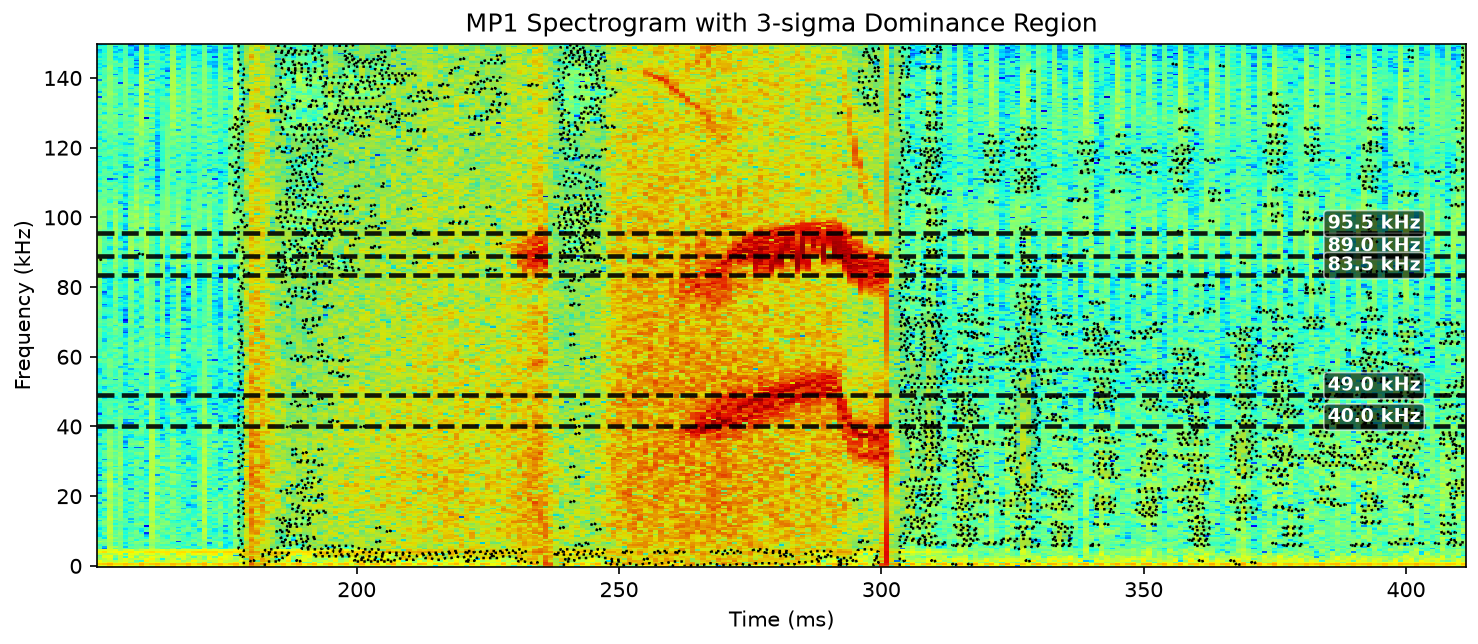
\includegraphics[width=0.86\textwidth]{Images/obj1_mode_identification/panels/mhd_analysis_objective1_88653_panel1_mp1_spectrogram_with_3_sigma_dominance_r.png}
  \caption[Mirnov MP1 spectrogram with statistical dominance threshold]{Mirnov MP1 PSD spectrogram ($500~\mathrm{Hz}$ resolution) with $3\sigma$ dominance contours over $150.0\text{--}350.0~\mathrm{ms}$ in shot \#88653.}
  \label{fig:obj1_spectrogram}
\end{figure}
Figure~\ref{fig:obj1_spectrogram} showed the MP1 STFT spectrogram for shot \#88653, isolating fluctuations that exceeded the $3\sigma$ pre-plasma noise baseline for $\geq 2~\mathrm{ms}$. After a brief burst near $230\text{--}236~\mathrm{ms}$, two dominant bands persisted across late $\mathrm{ECH}+\mathrm{NBI}$ and $\mathrm{NBI}$-only heating ($259.1\text{--}300.4~\mathrm{ms}$): the primary mode shifted from a mean of $87.5~\mathrm{kHz}$ to $86.5~\mathrm{kHz}$ across ECH switch-off, while the secondary mode dropped from $45.8~\mathrm{kHz}$ to $39.7~\mathrm{kHz}$. Because MP1 sampled a single-point edge location without radial resolution, internal localization and 3D coupling were established by cross-correlating the 16 ECE channels against all 18 Mirnov coils (Section~\ref{subsubsec:obj1_radial}).

\begin{figure}[H]
  \centering
  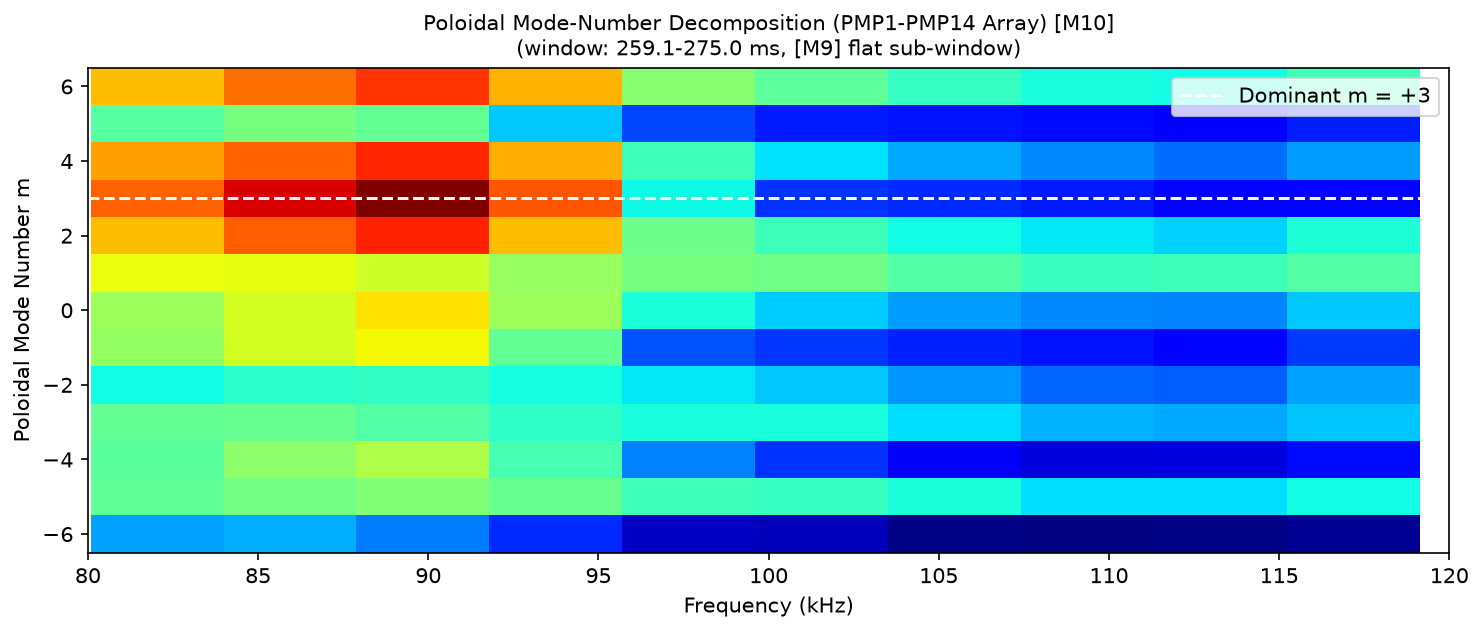
\includegraphics[width=0.85\textwidth]{Images/obj2_dynamics_and_structure/panels/mhd_analysis_objective2_structure_88653_80_120kHz_panel3_poloidal_mode_number_decomposition_pmp1.png}
  \caption[NUDFT poloidal mode decomposition for the primary mode]{NUDFT poloidal mode spectrum across PMP1--PMP14 for $80\text{--}120~\mathrm{kHz}$ over $259.1\text{--}275.0~\mathrm{ms}$ in shot \#88653.}
  \label{fig:obj1_poloidal_m}
\end{figure}
Figure~\ref{fig:obj1_poloidal_m} displayed the NUDFT poloidal mode decomposition across coils PMP1--PMP14 (after PMP1--PMP4 polarity correction) for the primary band ($80$--$120~\mathrm{kHz}$) over the $259.1$--$275.0~\mathrm{ms}$ flat-frequency sub-window of shot \#88653. Power concentrated at $84\text{--}95~\mathrm{kHz}$ along $m = +3$, while unequal poloidal coil spacing introduced residual sidelobe power into $m = +2, +4$ that required phase-concentration verification.

\begin{figure}[H]
  \centering
  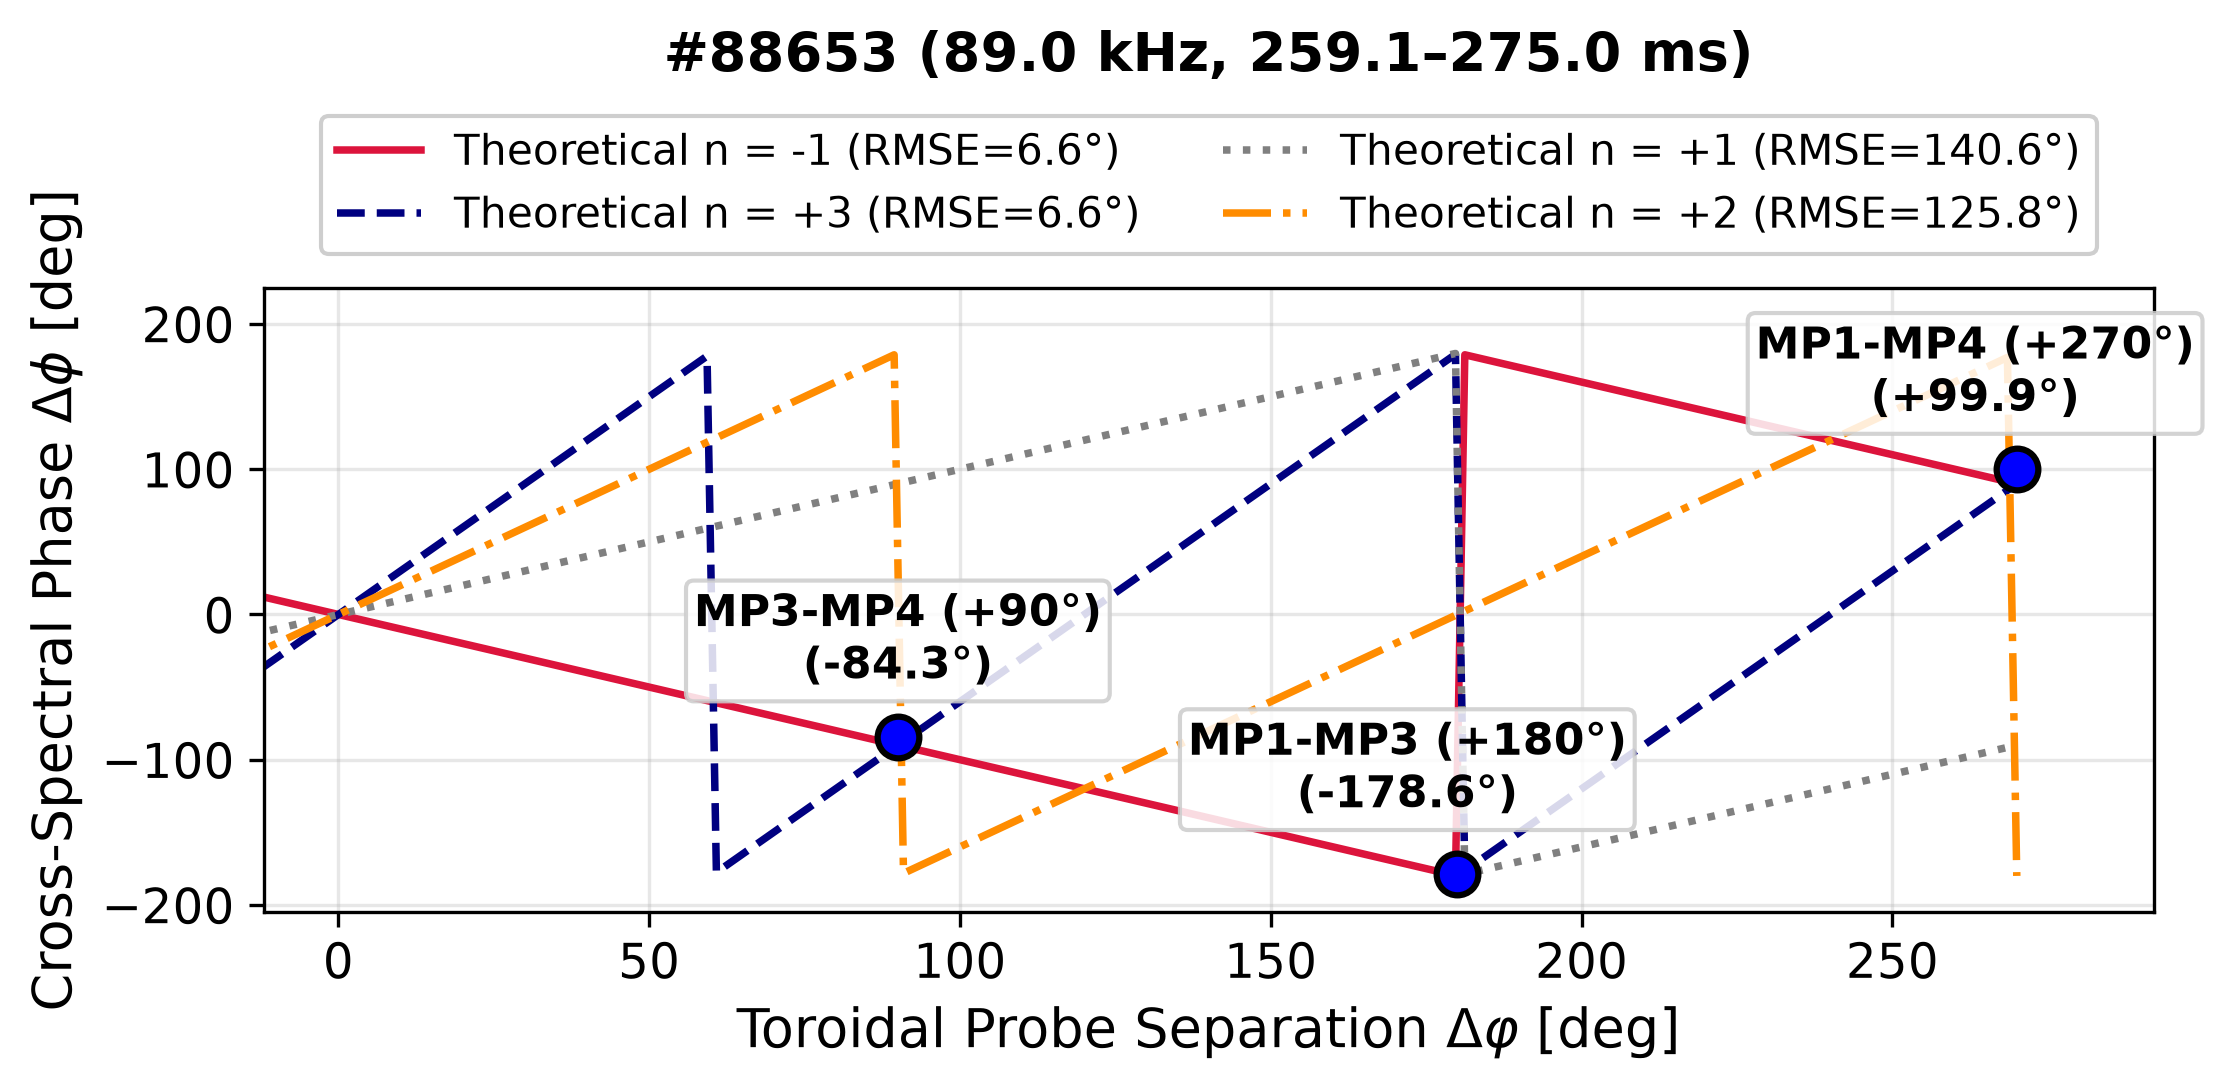
\includegraphics[width=0.85\textwidth]{Images/obj1_mode_identification/panels/mhd_primary_mode_toroidal_n_shot_88653_panel2_measured_phase_vs_theoretical_toroidal_p.png}
  \caption[Cross-probe phase versus toroidal angle for the primary mode]{Cross-spectral phase $\Delta\phi$ versus toroidal separation $\Delta\varphi$ at $89~\mathrm{kHz}$ ($259.1\text{--}275.0~\mathrm{ms}$, \#88653), fitting $n \equiv -1 \pmod 4$.}
  \label{fig:obj1_toroidal_n}
\end{figure}
Figure~\ref{fig:obj1_toroidal_n} compared the cross-spectral phase differences among coplanar coils MP1, MP3, and MP4 ($\Delta\phi = -84.3^\circ$ at $\Delta\varphi = +90^\circ$, $-178.6^\circ$ at $+180^\circ$, and $+99.9^\circ$ at $+270^\circ$) against candidate toroidal mode numbers for the $89~\mathrm{kHz}$ mode. The measured phases matched the degenerate aliases $n = -1$ and $n = +3$ ($\mathrm{RMSE} = 6.6^\circ$), rejecting $n = +1$ ($140.6^\circ$) and $n = +2$ ($125.8^\circ$). With three coplanar toroidal probes, the toroidal mode number was uniquely resolved modulo~4 ($n \equiv -1 \pmod 4$, \emph{supported}).

\begin{table}[H]
\centering
\footnotesize
\setlength{\tabcolsep}{2.6pt}
\renewcommand{\arraystretch}{1.15}
\caption[Spatial mode structure across heating phases and slices]{Spatial mode structure across heating phases and slices.}
\label{tab:mode_structure}
\sbox0{%
\begin{tabular}{llcccclccc}
\toprule
Band & Phase & \shortstack{$f$\\(kHz)} & \shortstack{$m$\\(-)} & \shortstack{$r_{\rm circ}$\\(-)} & \shortstack{Pol.\\Err. ($^\circ$)} & Label & \shortstack{Tor. $n$\\(mod 4, -)$^\dagger$} & \shortstack{Tor.\\RMSE ($^\circ$)} & \shortstack{Radial $\rho$ (-)\\(ECE12/13)} \\
\midrule
Secondary & ECH+NBI & 48.8 & $+1 \wedge +12$ & 0.832 & 24.9 & \emph{supported} & $-1$ & 22.7 & $0.29\text{--}0.47$ \\
Secondary & NBI only & 41.0 & $+1 \wedge +12$ & 0.854 & 25.7 & \emph{supported} & $-1$ & 19.3 & $0.29\text{--}0.47$ \\
Primary & ECH+NBI & 89.8 & $+3$ & 0.882 & 26.7 & \emph{supported} & $-1$ & 5.2 & $0.29\text{--}0.47$ \\
Primary & NBI only & 85.9 & $+3$ & 0.902 & 22.2 & \emph{supported} & $-1$ & 6.7 & $0.29\text{--}0.47$ \\
\shortstack[l]{Primary slice\\\#88653} & \shortstack[l]{post-transition\\291.4--291.8 ms} & -- & $+1$ & 0.608 & 65.0 & \emph{unresolved} & -- & -- & -- \\
\shortstack[l]{Primary slice\\\#88654} & \shortstack[l]{post-transition\\292.0--293.0 ms} & -- & $+3$ & 0.951 & 15.8 & \emph{supported} & -- & -- & -- \\
\bottomrule
\end{tabular}}
\ifdim\wd0>\textwidth\resizebox{\textwidth}{!}{\usebox0}\else\usebox0\fi
\par\smallskip Rows 1--4 correspond to shot \#88653; slices were analyzed individually. $^\dagger$Toroidal fit yields $n \bmod 4$ only (from three toroidal probes). \emph{Supported} requires $r_{\rm circ}\ge 0.70$ and mean poloidal error $\le 45^\circ$; ECE12/13 were calibrated via 3D \textsc{TRAVIS}. Post-transition slices were evaluated at 1~MHz using 256-sample segments with 192-sample overlap ($3$ and $12$ segments for $0.4$~ms and $1.0$~ms windows, respectively); ``--'' indicates parameters omitted in these single-frequency ($87$~kHz) short-window analyses.
\end{table}


\begin{figure}[H]
  \centering
  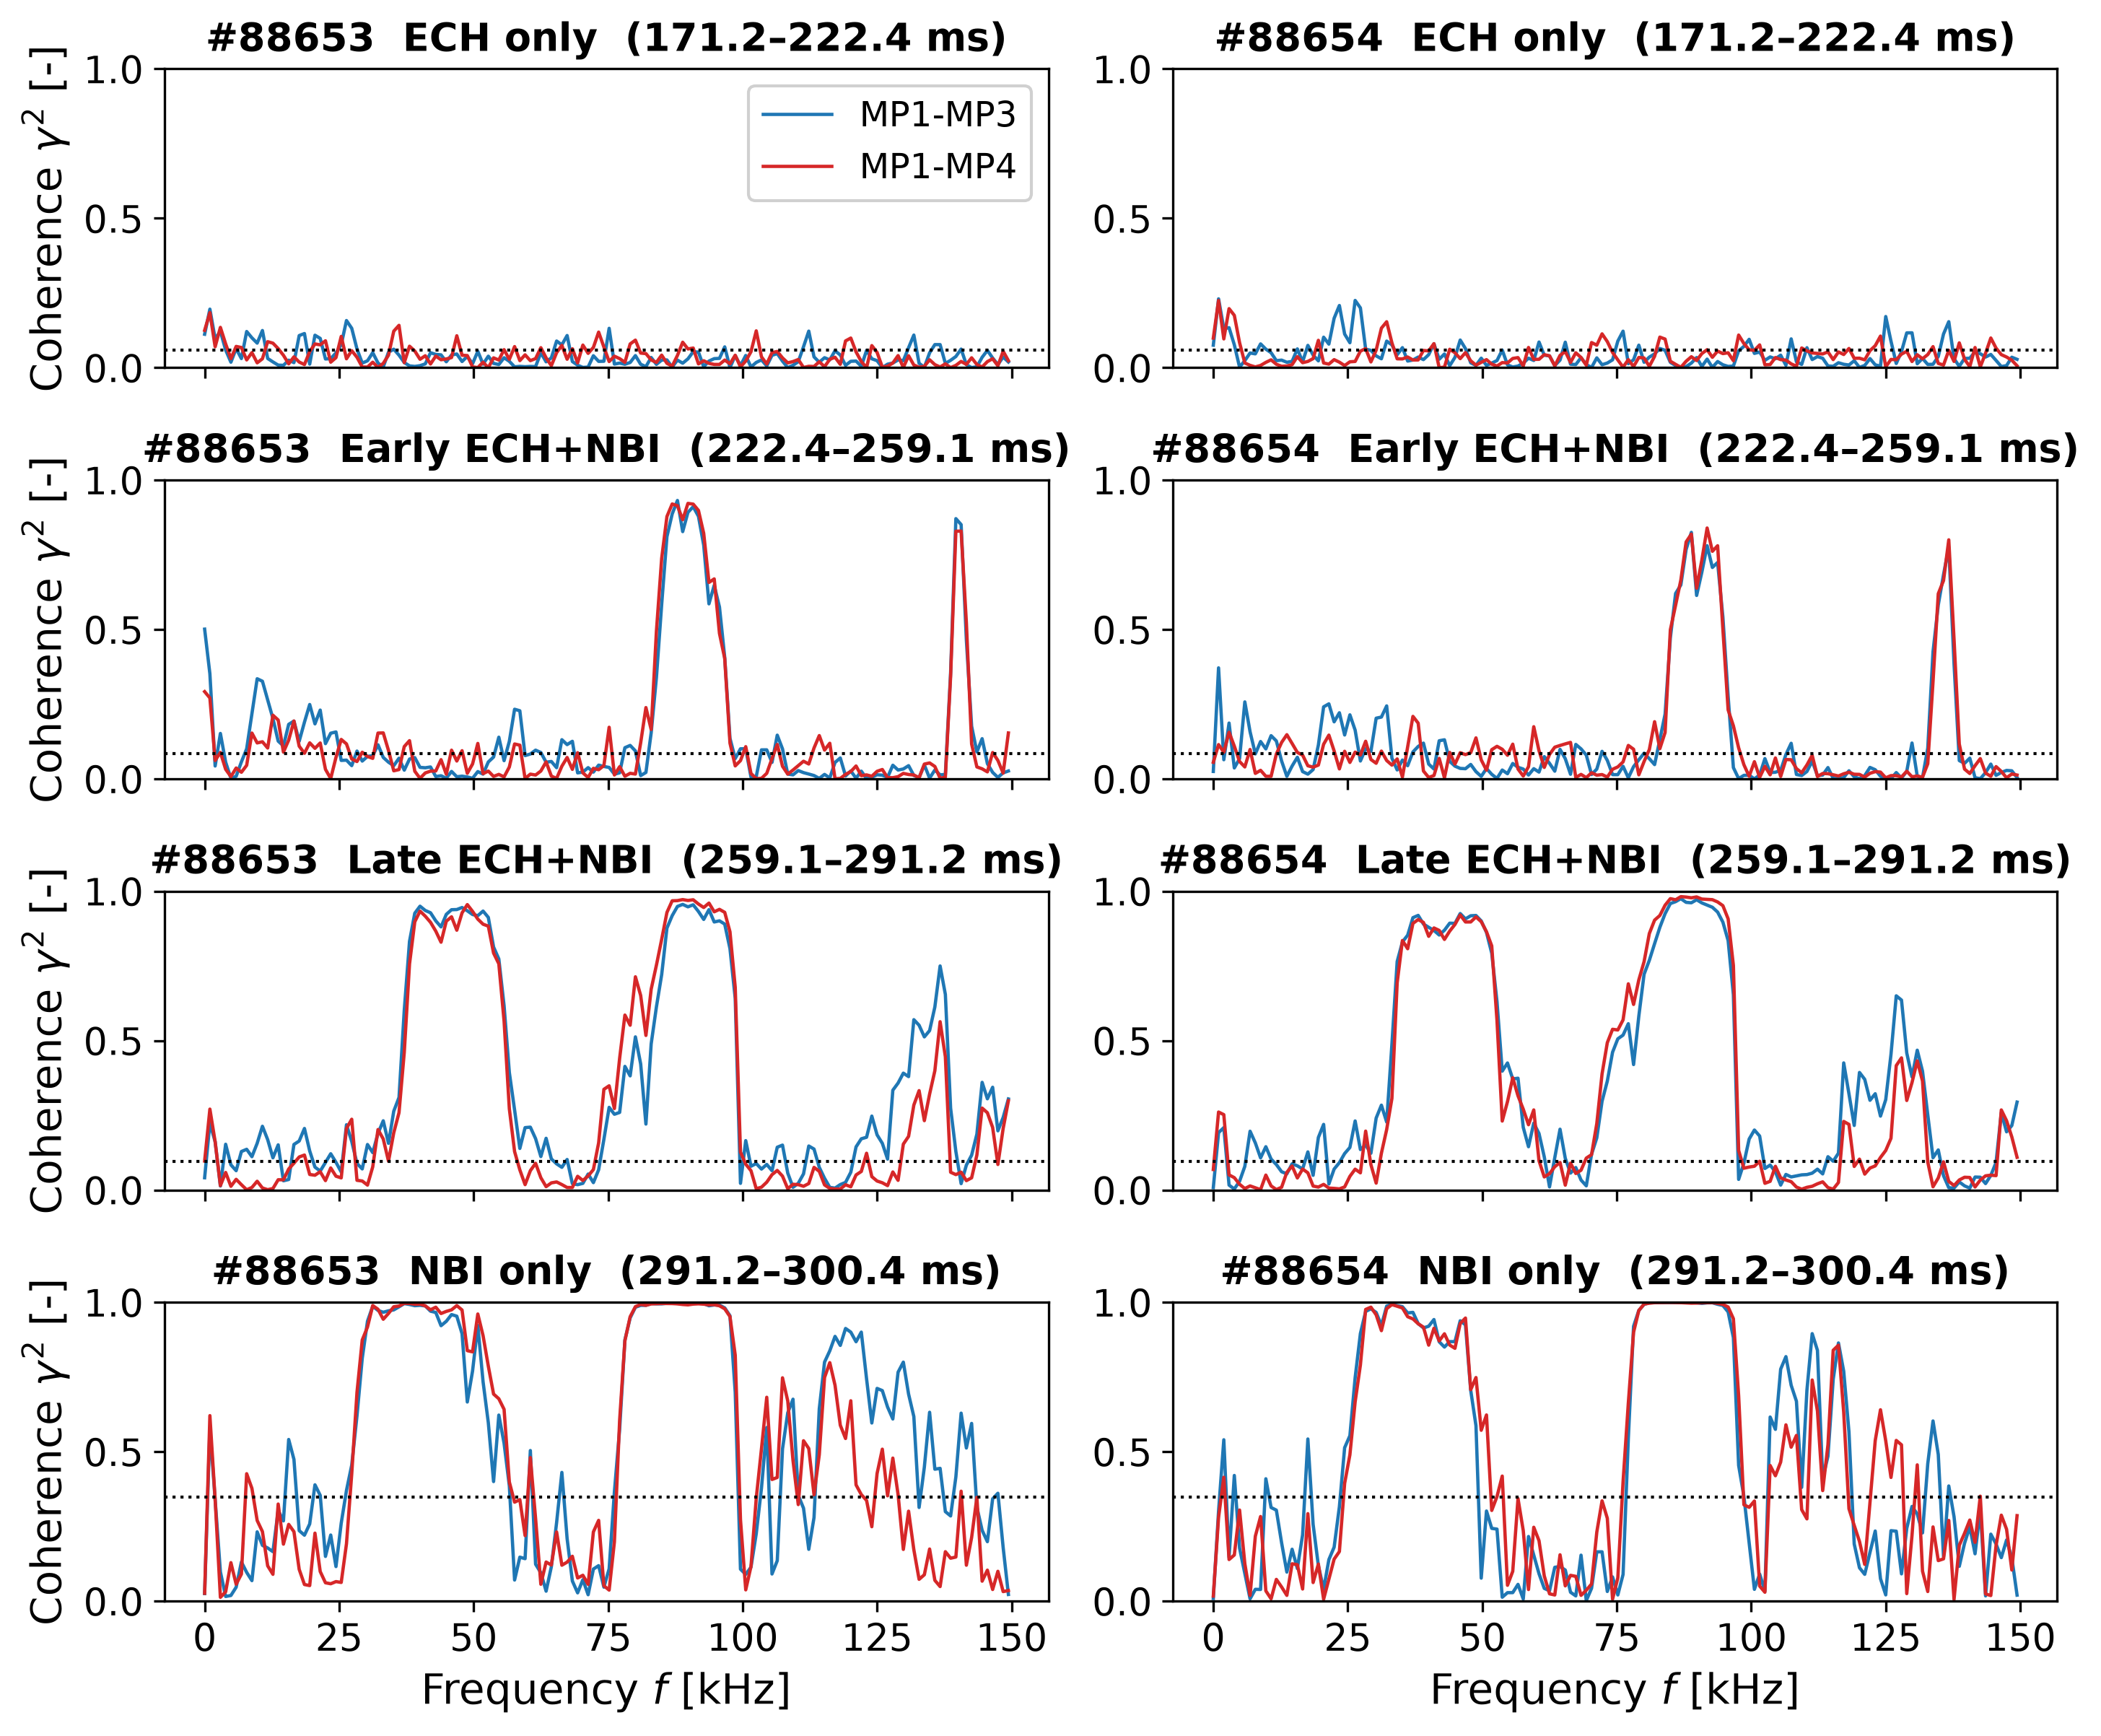
\includegraphics[width=0.88\textwidth]{Images/obj1_mode_identification/fig_coherence_spectra_both_shots.png}
  \caption[Probe coherence by heating phase]{Magnitude-squared coherence ($\gamma^2$) for MP1--MP3 and MP1--MP4 across heating phases in shots \#88653 (left) and \#88654 (right).}
  \label{fig:coherence_spectra}
\end{figure}
Table~\ref{tab:mode_structure} summarized the spatial mode structure across fixed heating windows and post-transition slices. In the primary band ($89.8~\mathrm{kHz}$ in $\mathrm{ECH}+\mathrm{NBI}$; $85.9~\mathrm{kHz}$ in $\mathrm{NBI}$-only), $m = +3$ achieved \emph{supported} status in both phases ($r_{\mathrm{circ}} = 0.882, 0.902$; errors $26.7^\circ, 22.2^\circ$) with $n \equiv -1 \pmod 4$ ($\mathrm{RMSE} = 5.2^\circ, 6.7^\circ$). In the brief post-transition $87~\mathrm{kHz}$ slices, $m = +3$ remained \emph{supported} in \#88654 ($292.0\text{--}293.0~\mathrm{ms}$, $12$ segments, $r_{\mathrm{circ}} = 0.951$, error $15.8^\circ$). In \#88653, however, the shorter $400$-sample slice ($291.4\text{--}291.8~\mathrm{ms}$, $3$ segments) became \emph{unresolved} ($m = +1$, $r_{\mathrm{circ}} = 0.608$, error $65.0^\circ$). Conversely, the secondary band ($48.8~\mathrm{kHz}$ in $\mathrm{ECH}+\mathrm{NBI}$; $41.0~\mathrm{kHz}$ in $\mathrm{NBI}$-only for \#88653) was resolved across both phases by a coexisting two-mode fit $(m_1 = +1, m_2 = +12)$. Both windows achieved \emph{supported} status ($r_{\mathrm{circ}} = 0.832, 0.854$; errors $24.9^\circ, 25.7^\circ$, spanning $11/14$ coils within $|\Delta\phi| \le 45^\circ$), with $n \equiv -1 \pmod 4$ ($\mathrm{RMSE} = 22.7^\circ, 19.3^\circ$). Single-harmonic fits ($m = +2$) failed with $81.1^\circ\text{--}100.9^\circ$ errors and $r_{\mathrm{circ}} = 0.58\text{--}0.63$. These results confirmed a global $m_1 = +1$ mode paired with a steep $m_2 = +12$ branch consistent with helical sideband coupling~\cite{Yamamoto_2020,Varela2024,Adulsiriswad_2024}. While $m_1 = +1$ was cleanly resolved, the $m_2 = +12$ branch approached the spatial Nyquist limit of the 14 irregular coils and could reflect either sideband coupling or spatial aliasing. Multi-phase coherence spectra (Figure~\ref{fig:coherence_spectra}, computed from $1024$-sample Hann segments with $50~\%$ overlap alongside the dotted optimistic $95~\%$ threshold assuming independent segments) confirmed reproducible dual-band excitation across both shots. During ECH-only ($171.2\text{--}222.4~\mathrm{ms}$), $\gamma^2$ stayed near noise; in early $\mathrm{ECH}+\mathrm{NBI}$ ($222.4\text{--}259.1~\mathrm{ms}$), it peaked above $0.8$ near $88$ and $140~\mathrm{kHz}$, before forming $\gamma^2 > 0.9$ plateaus ($35\text{--}55$ and $80\text{--}100~\mathrm{kHz}$) across late heating. Requiring NBI to destabilize both bands and their survival past ECH termination aligned with fast-ion-driven shear-Alfv\'en and EPM branches in Heliotron~J~\cite{Yamamoto_2020,Varela2015,Varela2024}.

\subsubsection{Radial Fluctuation Localization and Multi-Coil Magnetic Coupling}
\label{subsubsec:obj1_radial}

\begin{figure}[H]
  \centering
  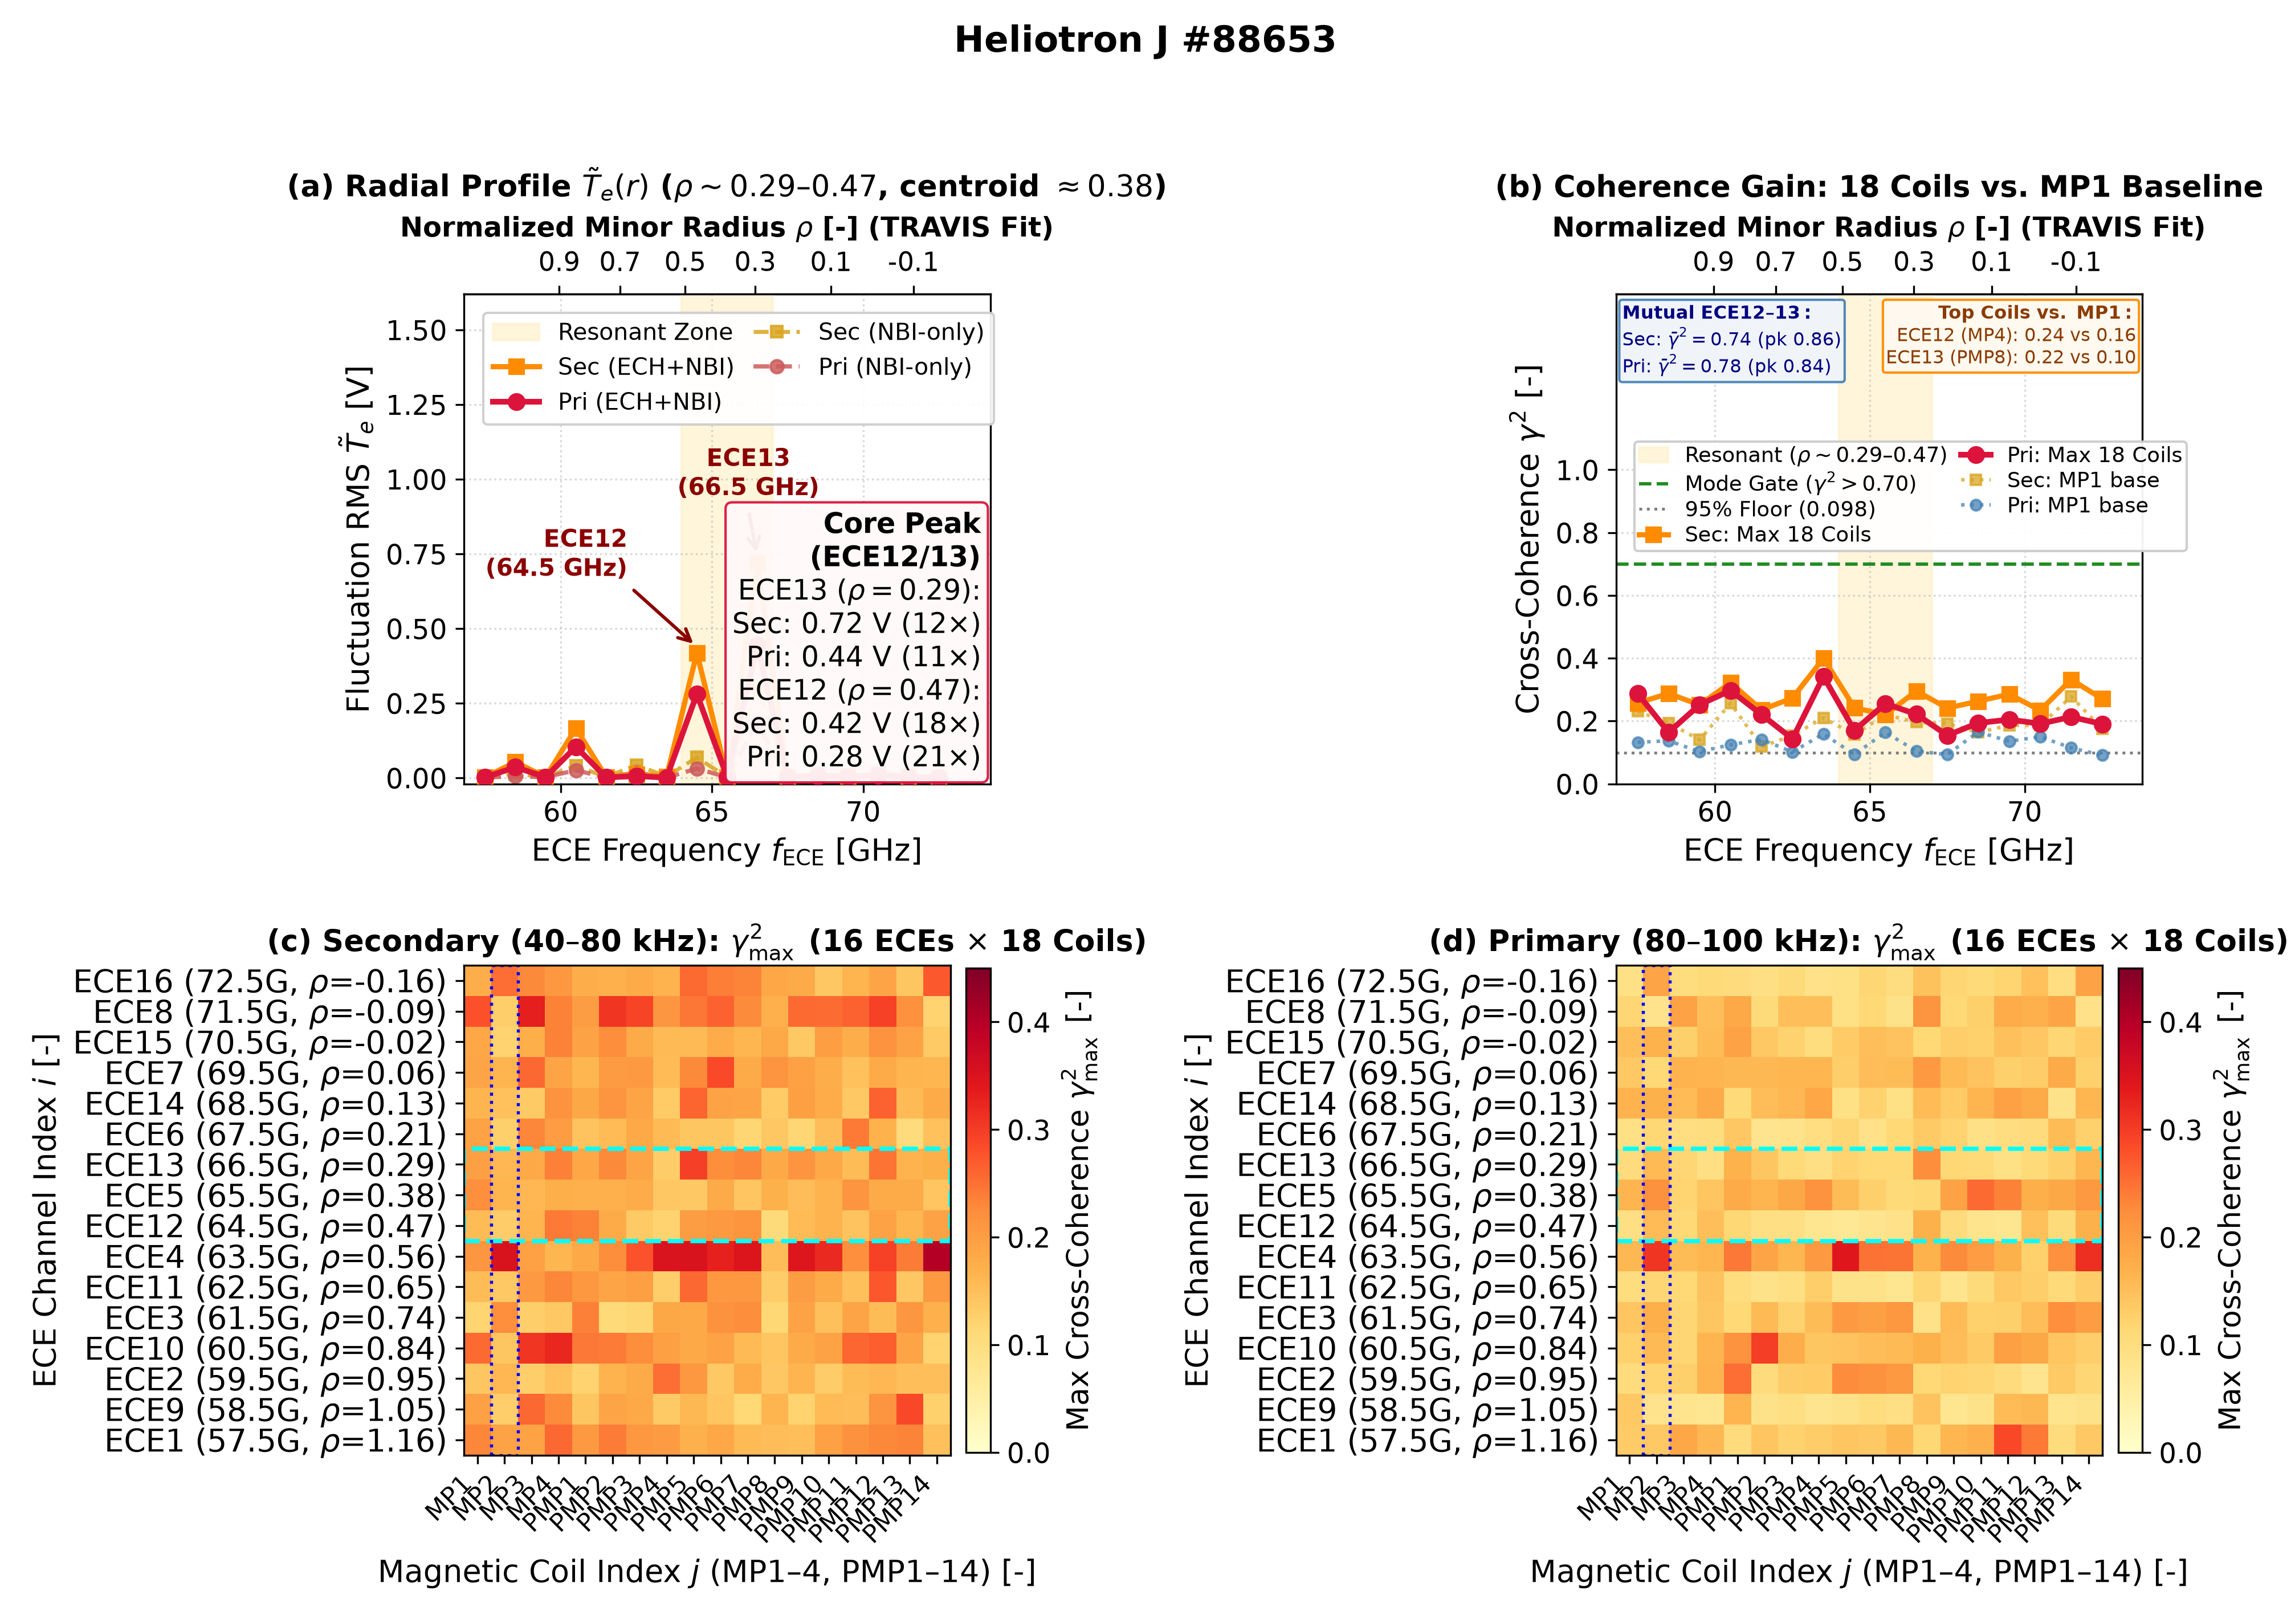
\includegraphics[width=\textwidth]{Images/obj1_mode_identification/mhd_ece_all_probes_radial_localization_88653.png}
  \caption[ECE radial localization and multi-coil magnetic coherence]{Radial localization and ECE--Mirnov coherence ($\mathrm{ECH}+\mathrm{NBI}$) in \#88653: (a)~ECE profile and (b--d)~$16\text{ ECE} \times 18\text{ Coil}$ coupling.}
  \label{fig:obj1_ece_radial}
\end{figure}

Figure~\ref{fig:obj1_ece_radial} presented radial localization and electromagnetic coupling across all 16 ECE channels ($57.5\text{--}72.5~\mathrm{GHz}$) and all 18 Mirnov coils (MP1--MP4, including non-coplanar MP2, and PMP1--PMP14). In Figure~\ref{fig:obj1_ece_radial}(a), the fluctuation RMS profile $\tilde{T}_e$ for both secondary ($40\text{--}80~\mathrm{kHz}$) and primary ($80\text{--}100~\mathrm{kHz}$) bands peaked sharply at \texttt{ECE12FAST} ($64.5~\mathrm{GHz}$, $\rho = 0.465$, $r \approx 7.91~\mathrm{cm}$) and \texttt{ECE13FAST} ($66.5~\mathrm{GHz}$, $\rho = 0.294$, $r \approx 4.99~\mathrm{cm}$). Together with the ${\approx}1~\mathrm{GHz}$ IF bandwidth and \textsc{TRAVIS} calibration (Eq.~(\ref{eqn:ece_travis_fit}), $\Delta \rho \approx 0.08\text{--}0.09$), these channels defined the core-to-mid gradient interval $\rho \approx 0.29\text{--}0.47$ ($\rho_{\mathrm{centroid}} \approx 0.380$, $r \approx 6.45~\mathrm{cm}$, within $\rho \in [0.25, 0.51]$).

During $\mathrm{ECH}+\mathrm{NBI}$ ($259.1\text{--}291.3~\mathrm{ms}$), secondary-band bandpass RMS reached $0.719~\mathrm{V}$ ($12.0\times$ pre-plasma noise) on \texttt{ECE13FAST} and $0.419~\mathrm{V}$ ($18.0\times$) on \texttt{ECE12FAST}; primary-band amplitudes reached $0.444~\mathrm{V}$ ($11.4\times$) and $0.281~\mathrm{V}$ ($21.1\times$), respectively. In the post-transition $\mathrm{NBI}$-only phase ($291.3\text{--}300.0~\mathrm{ms}$), \texttt{ECE13FAST} retained $0.302~\mathrm{V}$ ($5.0\times$) and $0.183~\mathrm{V}$ ($4.7\times$) across the secondary and primary bands. Adjacent \texttt{ECE12FAST}--\texttt{ECE13FAST} mutual coherence during $\mathrm{ECH}+\mathrm{NBI}$ reached $\gamma^2_{\mathrm{mean}} = 0.74$ ($\gamma^2_{\max} = 0.86$) in $40\text{--}80~\mathrm{kHz}$ and $0.78$ ($0.84$) in $80\text{--}100~\mathrm{kHz}$; given shared Bank~B baseline coupling ($\gamma^2_{\mathrm{mean}} \approx 0.74\text{--}0.83$ at $150\text{--}170~\mathrm{ms}$), mode confirmation rested jointly on the core RMS surge, selective $\mathrm{NBI}$-only peaks ($0.95\text{--}0.98$), and Mirnov coherence.

\paragraph*{Radial Phase Delay and Direction of Wave and Energy Propagation (\texttt{ECE13FAST} \texorpdfstring{$\leftrightarrow$}{<->} \texttt{ECE12FAST}).}
Cross-spectral density (CSD) phases $\Delta\phi_{13\to 12}(f) = \arg\langle \mathcal{H}(y_{13})\mathcal{H}^*(y_{12})\rangle$ and correlation lags $\Delta\tau_{13\to 12} = t_{12} - t_{13}$ resolved radial propagation between \texttt{ECE13FAST} ($\rho = 0.294$) and \texttt{ECE12FAST} ($\rho = 0.465$). This interval spanned $\Delta\rho = 0.171$ ($\Delta r \approx 2.92~\mathrm{cm}$) across carrier, envelope, and sawtooth bands. By convention, $\Delta\phi_{13\to 12} > 0$ ($\Delta\tau > 0$, channel $13$ leading channel $12$) indicated outward propagation ($13 \to 12$), consistent with outward cross-field heat transport and stored-energy degradation. Conversely, $\Delta\phi_{13\to 12} < 0$ ($\Delta\tau < 0$) denoted inward phase progression ($12 \to 13$).

This comparison (Figure~\ref{fig:ece_phase_delay}) revealed a clear physical dichotomy between the fast carrier phase velocity and wavepacket group transport. In the high-frequency carrier band during $\mathrm{ECH}+\mathrm{NBI}$, continuous phase delays were negative rather than quantized at $1~\mu\mathrm{s}$ steps. Secondary fluctuations ($40\text{--}80~\mathrm{kHz}$) gave $\Delta\phi_{13\to 12} = -10.8^\circ$ ($\Delta\tau = -0.51~\mu\mathrm{s}$, $r = +0.841$), while primary fluctuations ($80\text{--}100~\mathrm{kHz}$) gave $-12.7^\circ$ ($\Delta\tau = -0.39~\mu\mathrm{s}$, $r = +0.863$). These corresponded to an apparent inward phase velocity $v_{\mathrm{ph},r} \approx -57\text{ to }-75~\mathrm{km/s}$ (replicated in \#88654 at $-11.1^\circ$ and $-12.9^\circ$). Beyond wave propagation, steady negative phase offsets between adjacent ECE channels (both \texttt{ECE12FAST} and \texttt{ECE13FAST} belonged to local oscillator (LO) Bank~B) could also reflect an eigenmode radial phase tilt or minor sub-microsecond inter-channel IF or digitizer skew. Conversely, Hilbert envelopes $|\mathcal{H}|$ propagated outward: the primary envelope yielded $\Delta\tau_{\mathrm{env}} = +0.82~\mu\mathrm{s}$ ($r = 0.768$) in $\mathrm{ECH}+\mathrm{NBI}$, $+1.34~\mu\mathrm{s}$ in the sawtooth window, and $+1.37~\mu\mathrm{s}$ in $\mathrm{NBI}$-only ($v_{\mathrm{g},r} \approx +22\text{ to }+36~\mathrm{km/s}$). Mesoscopic sawtooth modulation ($277.0\text{--}294.0~\mathrm{ms}$) propagated outward at $+8.0~\mu\mathrm{s}$ (primary, $+4.0^\circ$, $r = +0.897$) and $+40.0~\mu\mathrm{s}$ (secondary, $+16.7^\circ$, $r = +0.671$). Similarly, the post-ECH thermal decay pulse ($0.35\text{--}2.2~\mathrm{kHz}$) moved outward at $+46.6~\mu\mathrm{s}$ ($+15.9^\circ$, $r = +0.782$ in \#88653; $+55.2~\mu\mathrm{s}$ in \#88654). Physically, the carrier phase reflected an inward-tilted radial eigenmode structure~\cite{zang2019observation,Zhong2024,luo2020measurement}, while wavepackets and thermal pulses transported energy radially outward across $\rho = 0.294\text{--}0.465$, consistent with core EPM/BAE observations~\cite{Weir2019,Kin2025}.

\begin{figure}[H]
  \centering
  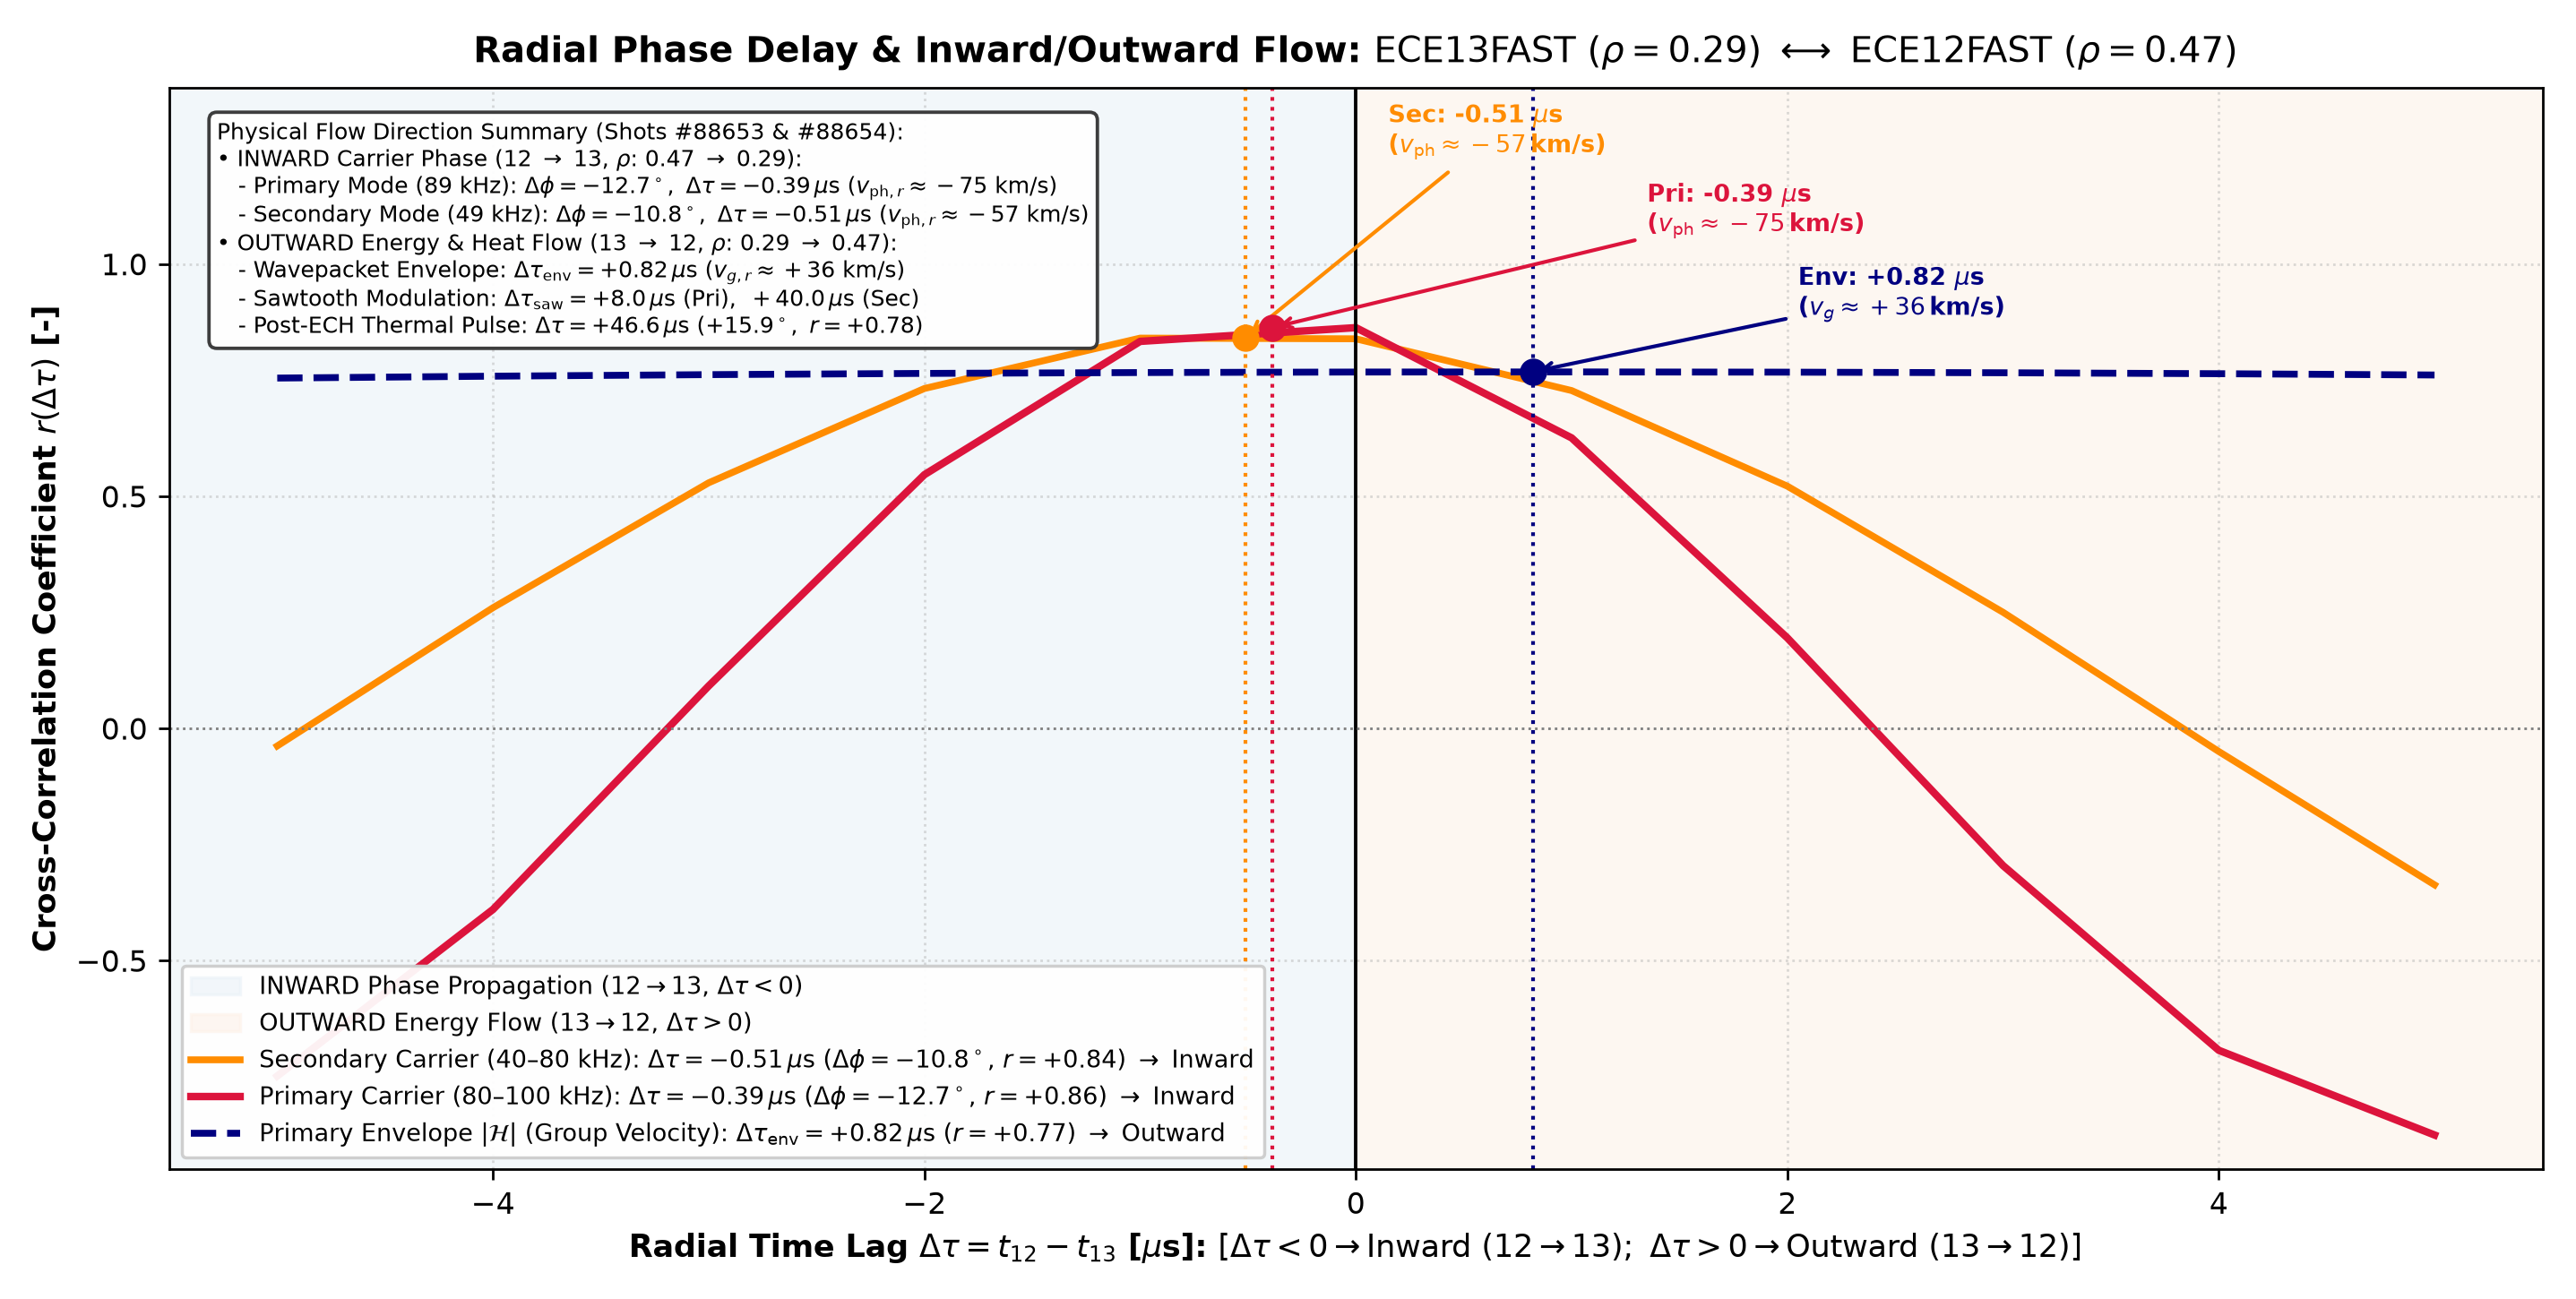
\includegraphics[width=0.95\textwidth]{Images/obj1_mode_identification/mhd_ece12_13_phase_delay_flow_88653.png}
  \caption[Radial phase delay and wavepacket group propagation between ECE13FAST and ECE12FAST]{Lagged cross-correlation $r(\Delta\tau)$ between \texttt{ECE13FAST} ($\rho = 0.294$) and \texttt{ECE12FAST} ($\rho = 0.465$) during $\mathrm{ECH}+\mathrm{NBI}$ in shot \#88653, comparing inward carrier phase delays ($\Delta\tau < 0$) against outward wavepacket envelope transport ($\Delta\tau_{\mathrm{env}} = +0.82~\mu\mathrm{s}$).}
  \label{fig:ece_phase_delay}
\end{figure}

Scanning $16\text{ ECE} \times 18\text{ Coil}$ ECE--Mirnov coherence during $\mathrm{ECH}+\mathrm{NBI}$ (Figure~\ref{fig:obj1_ece_radial}(b--d)) resolved a single-probe limitation and explained why cross-diagnostic $\gamma^2_{\max}$ stayed below internal ECE--ECE levels. Core ECE ($\tilde{T}_e$) versus vessel-wall Mirnov ($\mathrm{d}\tilde{B}_\theta/\mathrm{d}t$) separation, uncorrelated $70~\mathrm{GHz}$ ECH broadband power, and $17.4~\%$ \texttt{ECE13FAST} rail clipping diluted $\gamma^2$ on MP1 ($0.093\text{--}0.104$ primary; $0.156\text{--}0.196$ secondary), yet multi-coil scanning cleared the $95~\%$ floor ($\gamma^2_{95\%} = 0.049, 0.098$ for $N_{\mathrm{fft}}=1024, 2048$). In $40\text{--}80~\mathrm{kHz}$, coherence reached $\gamma^2 = 0.322$ (\texttt{ECE10FAST} / MP4), $0.295$ (\texttt{ECE13FAST} / PMP5), and $0.242$ (\texttt{ECE12FAST} / MP4), with $|r_{\mathrm{env}}| = 0.287$ (\texttt{ECE12FAST} / MP4). In $80\text{--}100~\mathrm{kHz}$, coherence reached $0.297$ (\texttt{ECE10FAST} / PMP2) and $0.222$ (\texttt{ECE13FAST} / PMP8), with $|r_{\mathrm{car}}| = 0.122$ (\texttt{ECE5FAST} / MP2) and $|r_{\mathrm{env}}| = 0.205$ (\texttt{ECE9FAST} / PMP12) and $0.199$ (\texttt{ECE12FAST} / PMP12).

Switching off the $70~\mathrm{GHz}$ ECH source in the $\mathrm{NBI}$-only phase ($291.3\text{--}300.0~\mathrm{ms}$) eliminated RF pickup and substantially strengthened ECE--Mirnov coupling across internal and outer-gradient channels. Within the secondary band, $|r_{\mathrm{car}}|$ reached $0.404$ (\texttt{ECE12FAST} / MP4) and $0.400$ (\texttt{ECE13FAST} / MP4), while $|r_{\mathrm{env}}|$ reached $0.553$ (\texttt{ECE13FAST} / MP4) and coherence peaked at $\gamma^2 = 0.799$ (\texttt{ECE13FAST} / PMP13 at $44.9~\mathrm{kHz}$) and $0.661$ (\texttt{ECE12FAST} / PMP2). For the primary mode, carrier correlation reached $|r_{\mathrm{car}}| = 0.411$ (\texttt{ECE11FAST} / PMP14) and $0.284$ (\texttt{ECE13FAST} / MP3), and envelope correlation reached $|r_{\mathrm{env}}| = 0.586$ (\texttt{ECE11FAST} / MP2) and $0.518$ (\texttt{ECE13FAST} / MP3). At the $86.0~\mathrm{kHz}$ peak, off-midplane coil MP2 ranked highest ($\gamma^2 = 0.360$ on \texttt{ECE11FAST} / MP2, $\rho = 0.65$; $0.359$ on \texttt{ECE10FAST} / MP2, $\rho = 0.84$), while band-maximum coherence reached $\gamma^2 = 0.670$ (\texttt{ECE13FAST} / PMP2). Although part of the broadband coherence across core-to-outer-gradient ECE channels (\texttt{ECE13FAST} to \texttt{ECE10FAST}, $\rho = 0.29\text{--}0.84$) during $291.3\text{--}293.5~\mathrm{ms}$ reflected post-ECH equilibrium relaxation, the step-free steady tail ($294.2\text{--}300.0~\mathrm{ms}$) confirmed persistent mode-specific coherence. Tail coherence exceeded the $95~\%$ floor at $\gamma^2 = 0.350$ on \texttt{ECE13FAST} / PMP11 ($40\text{--}80~\mathrm{kHz}$), alongside $0.301$ on \texttt{ECE14FAST} / PMP13 and $0.275$ on \texttt{ECE15FAST} / MP2 ($80\text{--}100~\mathrm{kHz}$).

\begin{figure}[H]
  \centering
  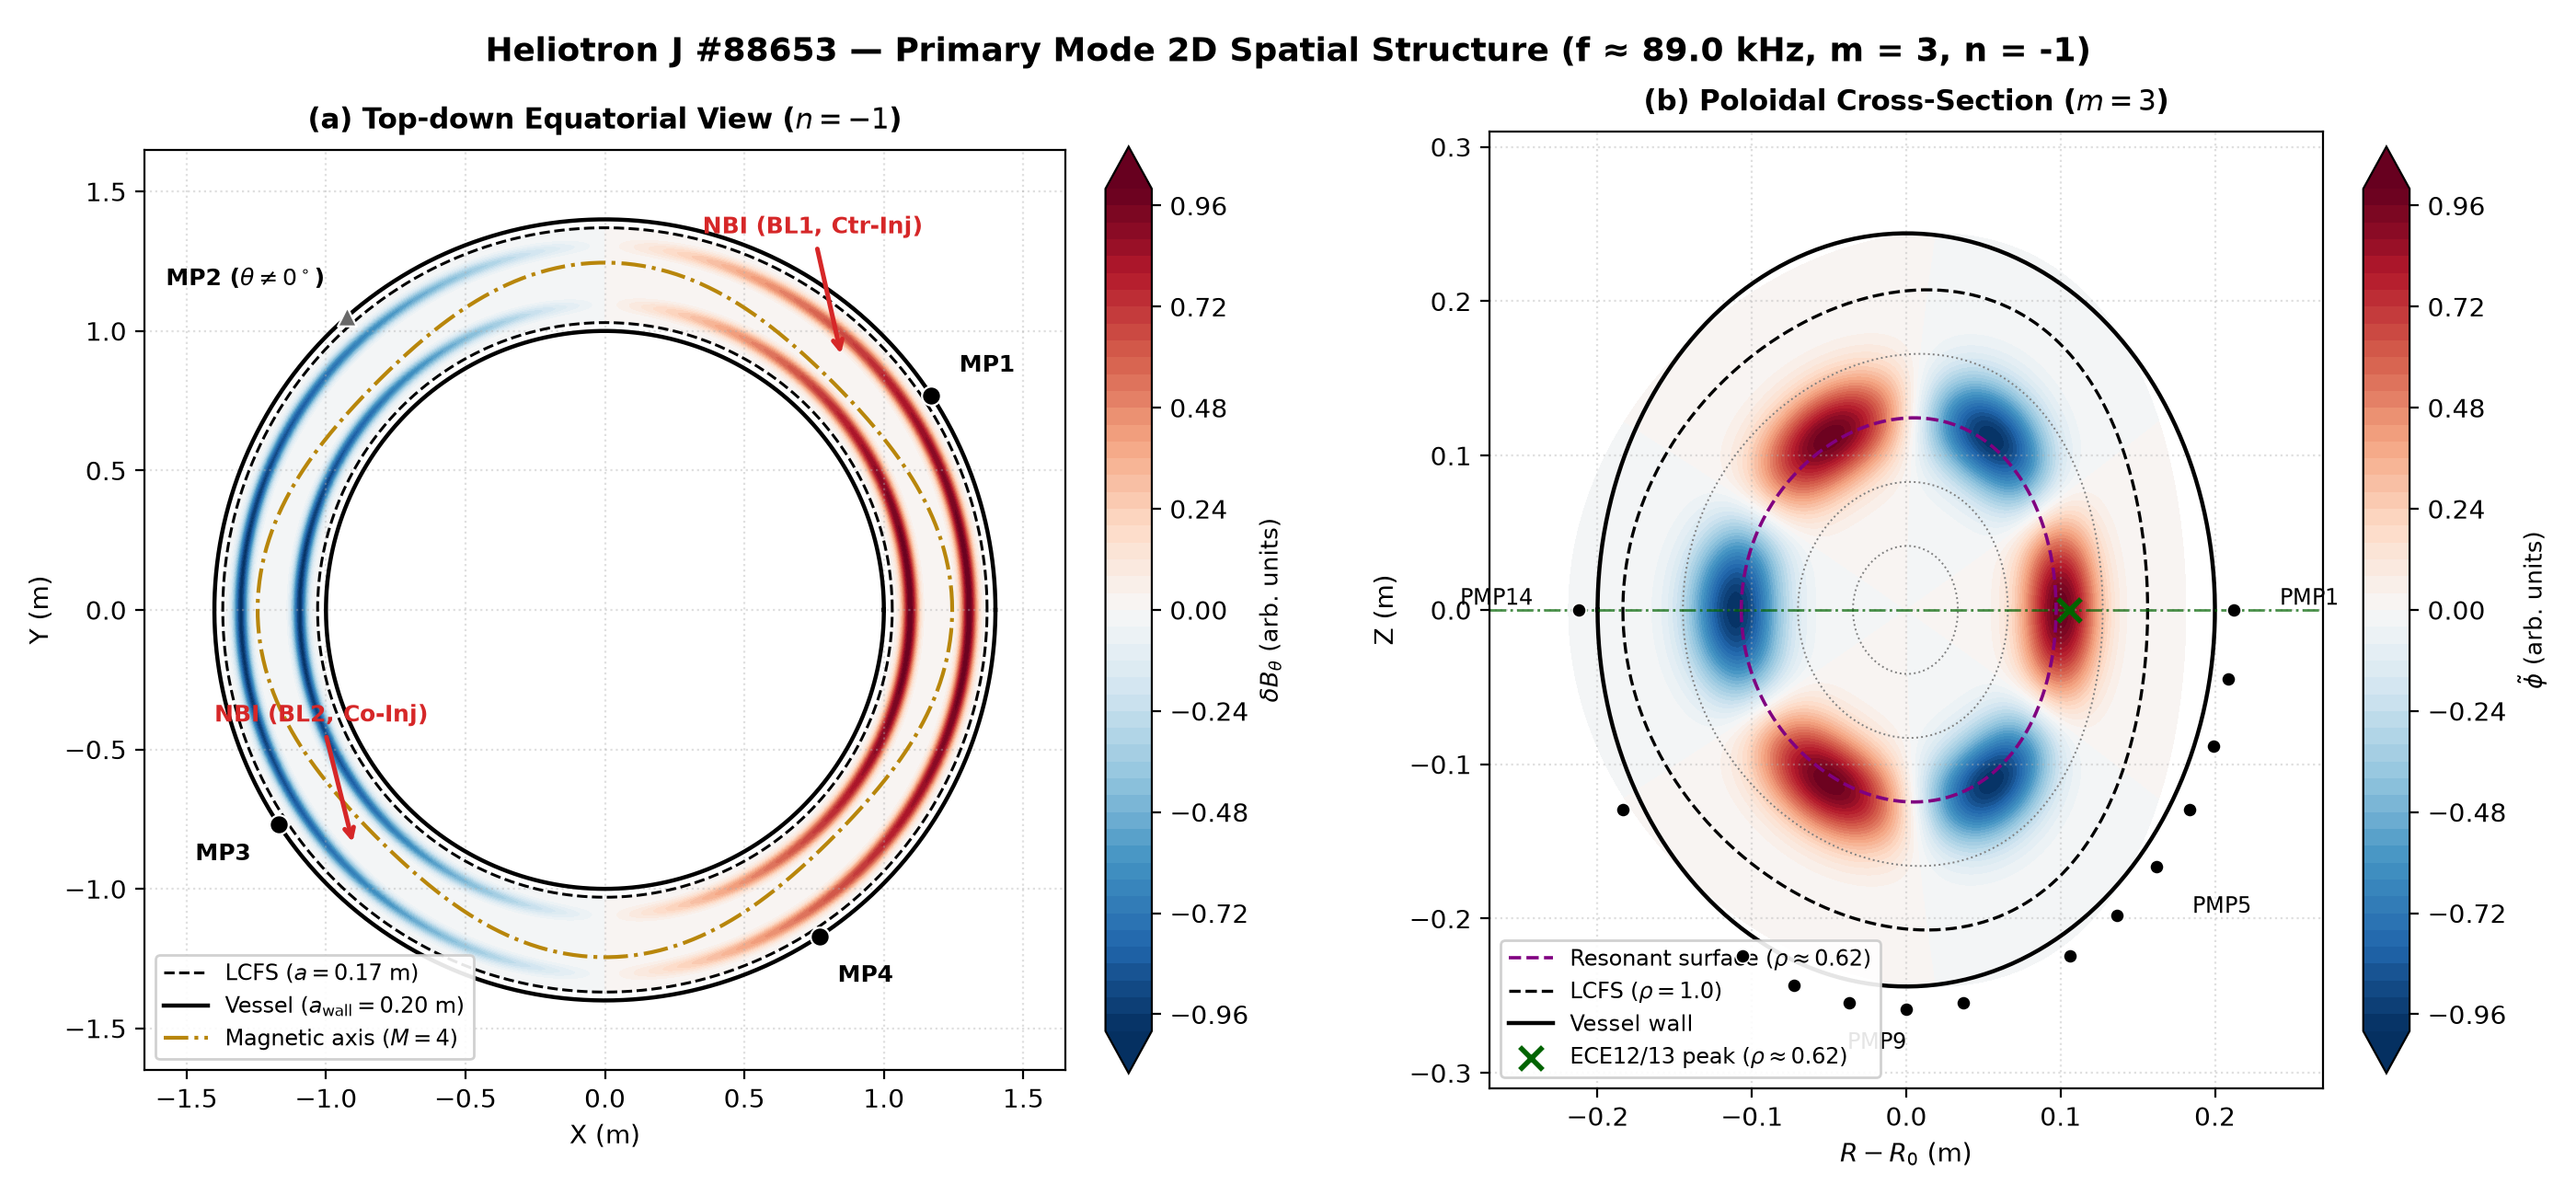
\includegraphics[width=0.98\textwidth]{Images/obj2_dynamics_and_structure/mhd_mode_spatial_map_2d_88653.png}
  \caption[2D schematic representation of the fitted MHD mode structures]{2D schematic of fitted MHD mode structures in shot \#88653: (a)~equatorial view and (b, c)~poloidal cross-sections.}
  \label{fig:obj1_spatial_map_2d}
\end{figure}

Figure~\ref{fig:obj1_spatial_map_2d} synthesized these structural findings into a 2D schematic representation of the fitted mode harmonics (normalized) overlaid on the equilibrium and diagnostic layout within the last closed flux surface (LCFS, $\rho = 1.0$, $a = 0.17~\mathrm{m}$): panel~(a) showed the equatorial plane ($Z = 0$) with $n \equiv -1 \pmod 4$, toroidal probes MP1--MP4, and the ECE sightline, whereas panels~(b, c) displayed poloidal cross-sections over PMP1--PMP14 for the secondary ($m_1 = +1 \wedge m_2 = +12$) and primary ($m = +3$) harmonics across the $\rho \sim 0.29\text{--}0.47$ resonant zone. Combining the poloidal numbers ($m=+3$ primary; coexisting $m_1=+1 \wedge m_2=+12$ secondary), toroidal mode number ($n \equiv -1 \pmod 4$), and radial birth zone localized the instability in the core-to-mid gradient region. This spatial co-localization of the $m/n = 3/-1$ and $(1, 12)/-1$ modes established the shared resonant layer governing energetic-particle drive, rational-surface alignment, and nonlinear wave--wave interactions.

\subsubsection{Dynamic Behavior and Frequency Evolution}
\label{subsubsec:obj1_dynamics}
As shown in Figures~\ref{fig:obj1_spectrogram} and~\ref{fig:coherence_spectra}, both primary ($80\text{--}100~\mathrm{kHz}$) and secondary ($35\text{--}55~\mathrm{kHz}$) modes persisted throughout late $\mathrm{ECH}+\mathrm{NBI}$ ($259.1\text{--}291.3~\mathrm{ms}$). Both bands chirped upward over $259\text{--}275~\mathrm{ms}$ before stabilizing, then survived into post-ECH $\mathrm{NBI}$-only heating ($291.3\text{--}300.4~\mathrm{ms}$, $\gamma^2 > 0.95$) with downward frequency sweeping until NBI shut-off (\emph{supported}, though the brief $9.1~\mathrm{ms}$ window bounded spectral resolution). Comparable upward chirping followed by downward relaxation during fast-ion drive and $T_e$ decay characterized resonant EPM and BAE branches~\cite{Zhong2024,Varela2023,Yamamoto_2020}.

\subsubsection{Response to ECH Switch-Off}
\label{subsubsec:obj1_ech_off}

\begin{table}[H]
\centering
\small
\setlength{\tabcolsep}{4.5pt}
\renewcommand{\arraystretch}{1.15}
\caption[Heating phases and Mirnov spectral summary for shot \#88653]{Heating phases and Mirnov spectral summary for shot \#88653.}
\label{tab:discharge_phases}
\begin{tabular}{lccccrl}
\toprule
Phase & \shortstack{Coherence\\window (ms)} & \shortstack{RMS\\window (ms)} & \shortstack{MP1\\RMS (V)} & \shortstack{Peak\\$\gamma^2$ (-)} & \shortstack{Power /\\threshold (-)} & \shortstack{Discrete\\modes (kHz)} \\
\midrule
Pre-plasma & 150.0--171.2 & 150.0--171.2 & 0.016 & 0.765 & 0.7 & none \\
ECH only & 171.2--222.4 & 171.0--222.0 & 0.040 & 0.158 & 33.8 & none \\
Early ECH+NBI & 222.4--259.1 & 222.0--259.0 & 0.087 & 0.931 & 450.6 & 87.9, 139.6 \\
Late ECH+NBI & 259.1--291.2 & 259.0--291.0 & 0.274 & 0.972 & 7052.3 & 40.0, 88.9 \\
NBI only & 291.2--300.4 & 291.2--300.4 & 0.281 & 0.997 & 9232.6 & \shortstack[l]{37.1, 50.8,\\86.9, 115.2} \\
\shortstack[l]{Post-heating\\decay} & 300.4--350.0 & 300.4--350.0 & 0.054 & 0.990 & 131.4 & \shortstack[l]{31.2, 35.2, 41.0,\\48.8 (+5)} \\
\bottomrule
\end{tabular}
\par\smallskip{\footnotesize Peak $\gamma^2$ computed from MP1--MP3; RMS amplitude evaluated over the specified time intervals. Pre-plasma exhibits no spectral line above the detection threshold, so its $\gamma^2$ value does not represent a coherent mode. Line frequencies correspond to fixed phase windows and may differ by one STFT bin from those in Table~\ref{tab:mode_structure}.}
\end{table}


\begin{figure}[htbp]
  \centering
  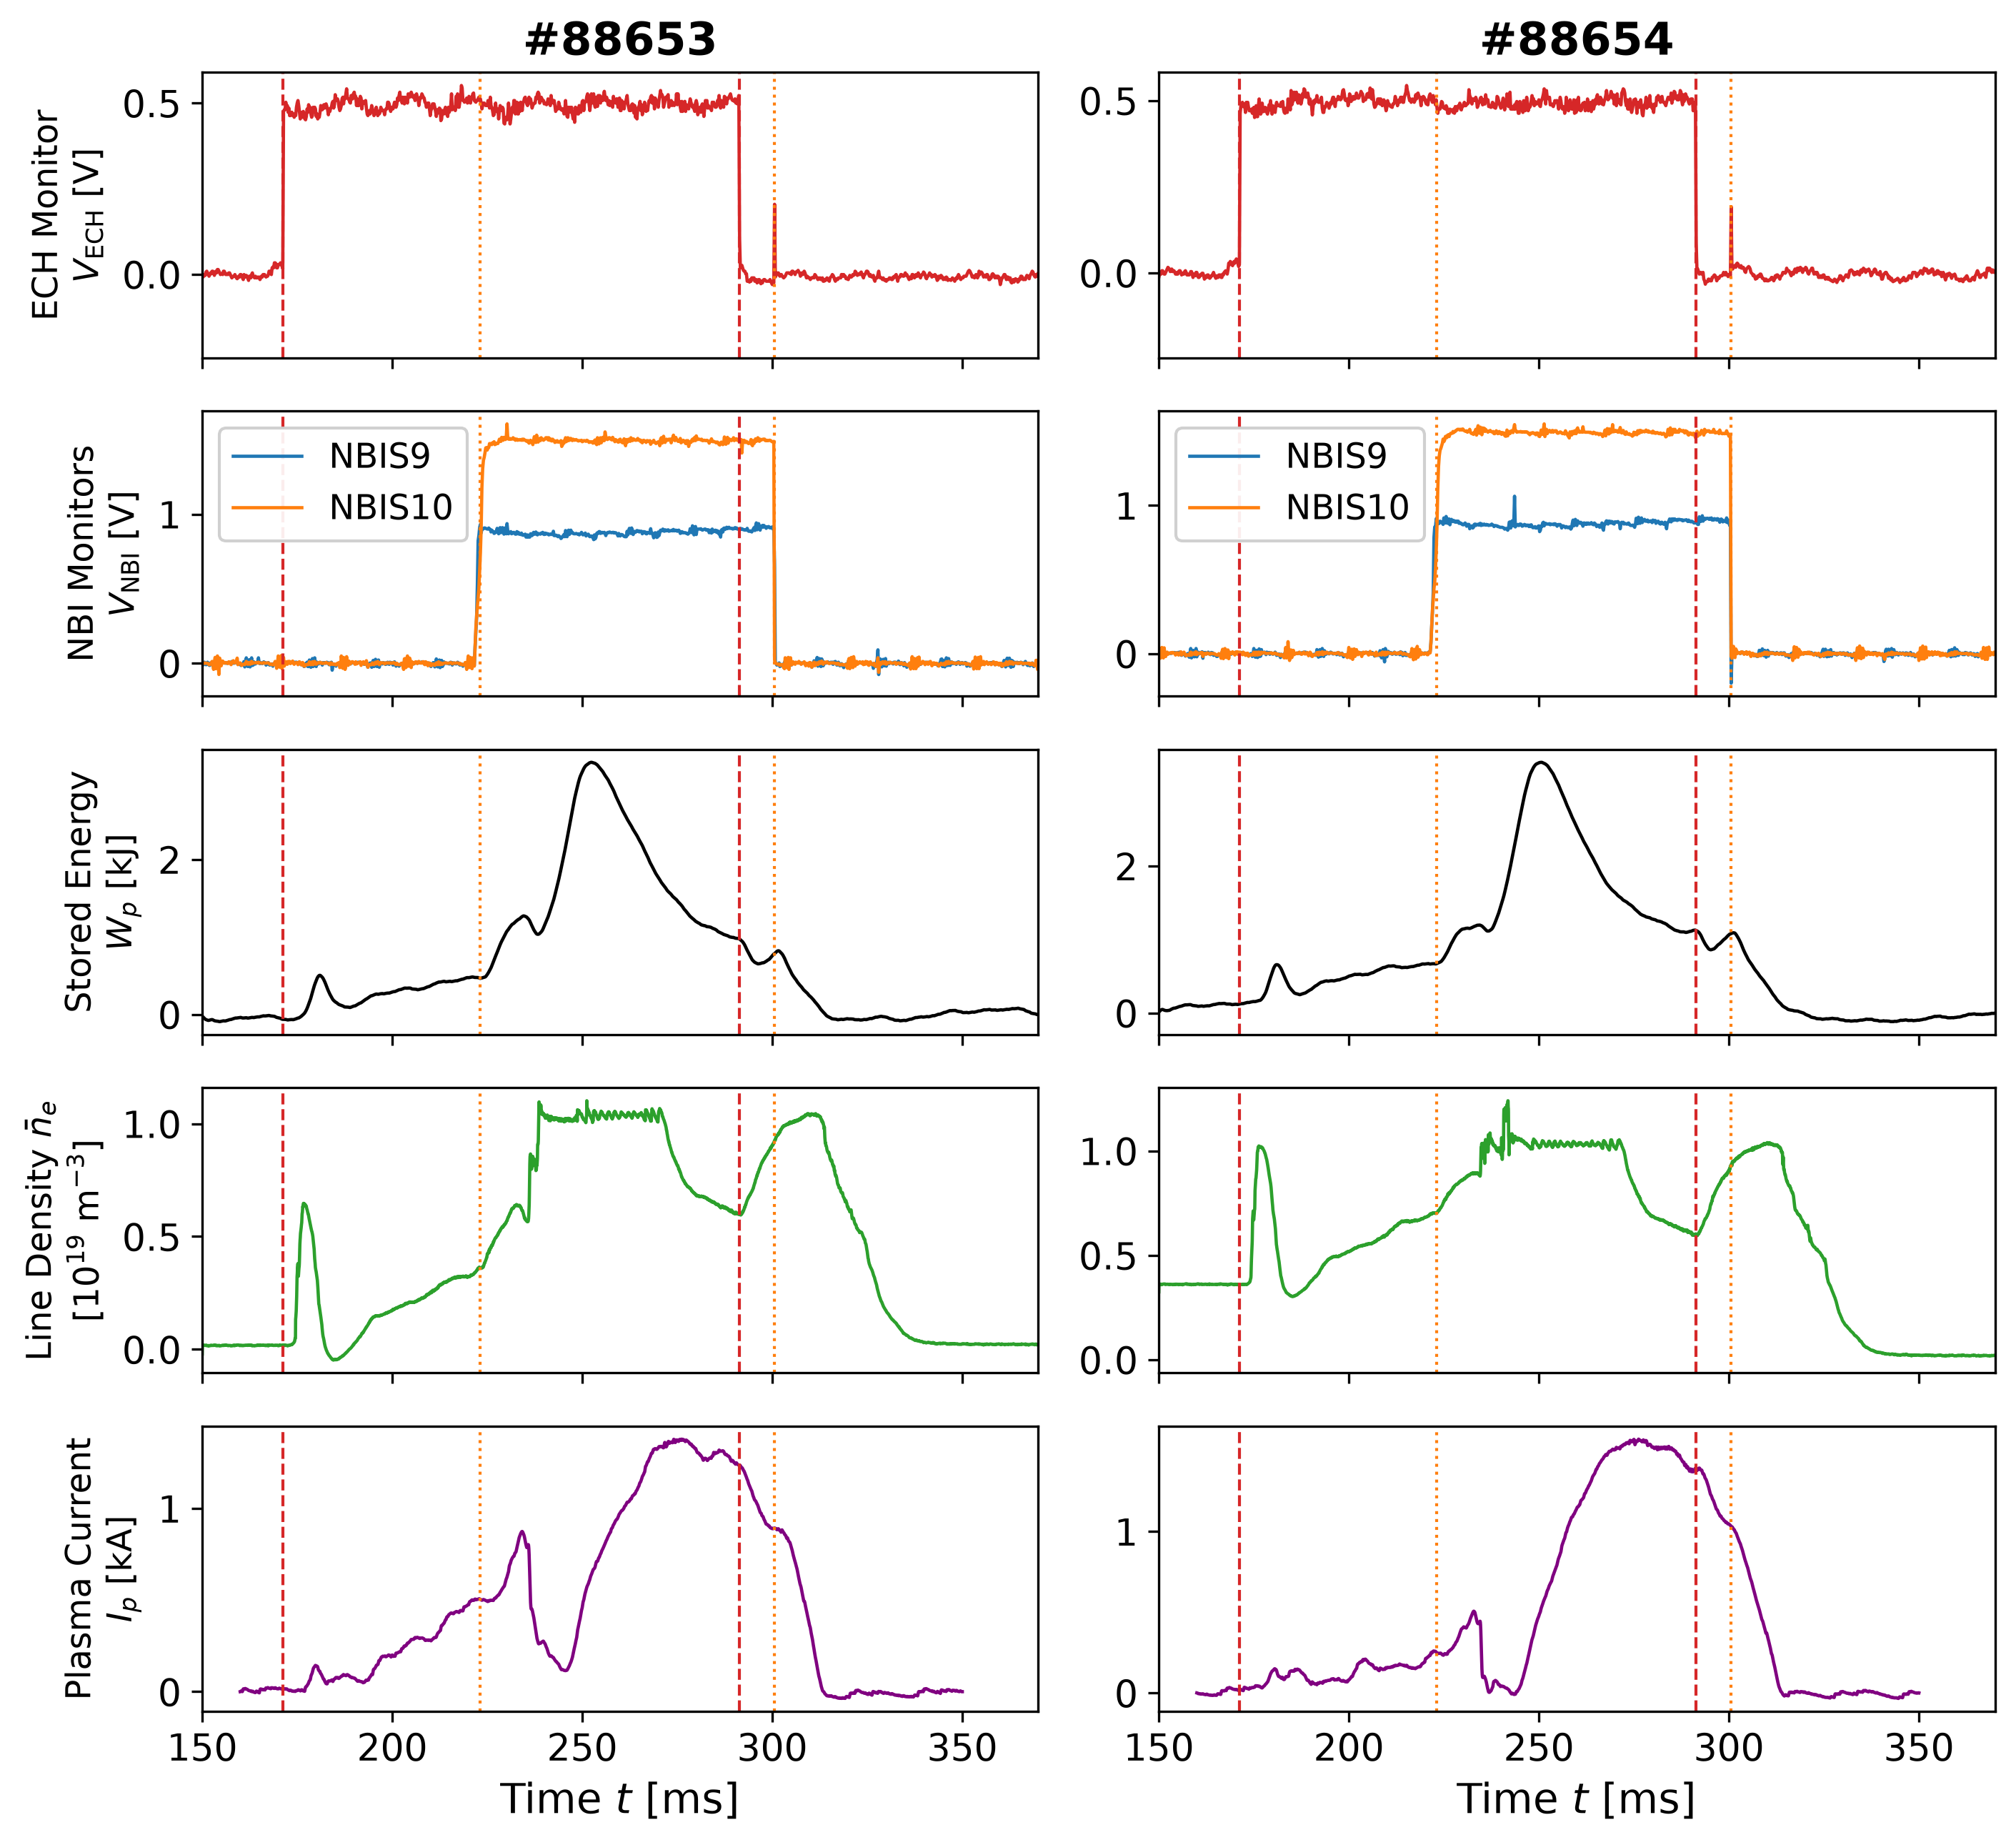
\includegraphics[width=0.80\textwidth]{Images/obj2_dynamics_and_structure/panels/fig_heating_timeline_both_shots.png}
  \caption[Heating signals and \texorpdfstring{$I_p$}{Ip}, both shots]{Heating traces (ECH, NBIS9, NBIS10), $W_p$, $n_e$, and $I_p$ ($150\text{--}370~\mathrm{ms}$) for shots \#88653 and \#88654.}
  \label{fig:heating_timeline}
\end{figure}

\begin{figure}[htbp]
  \centering
  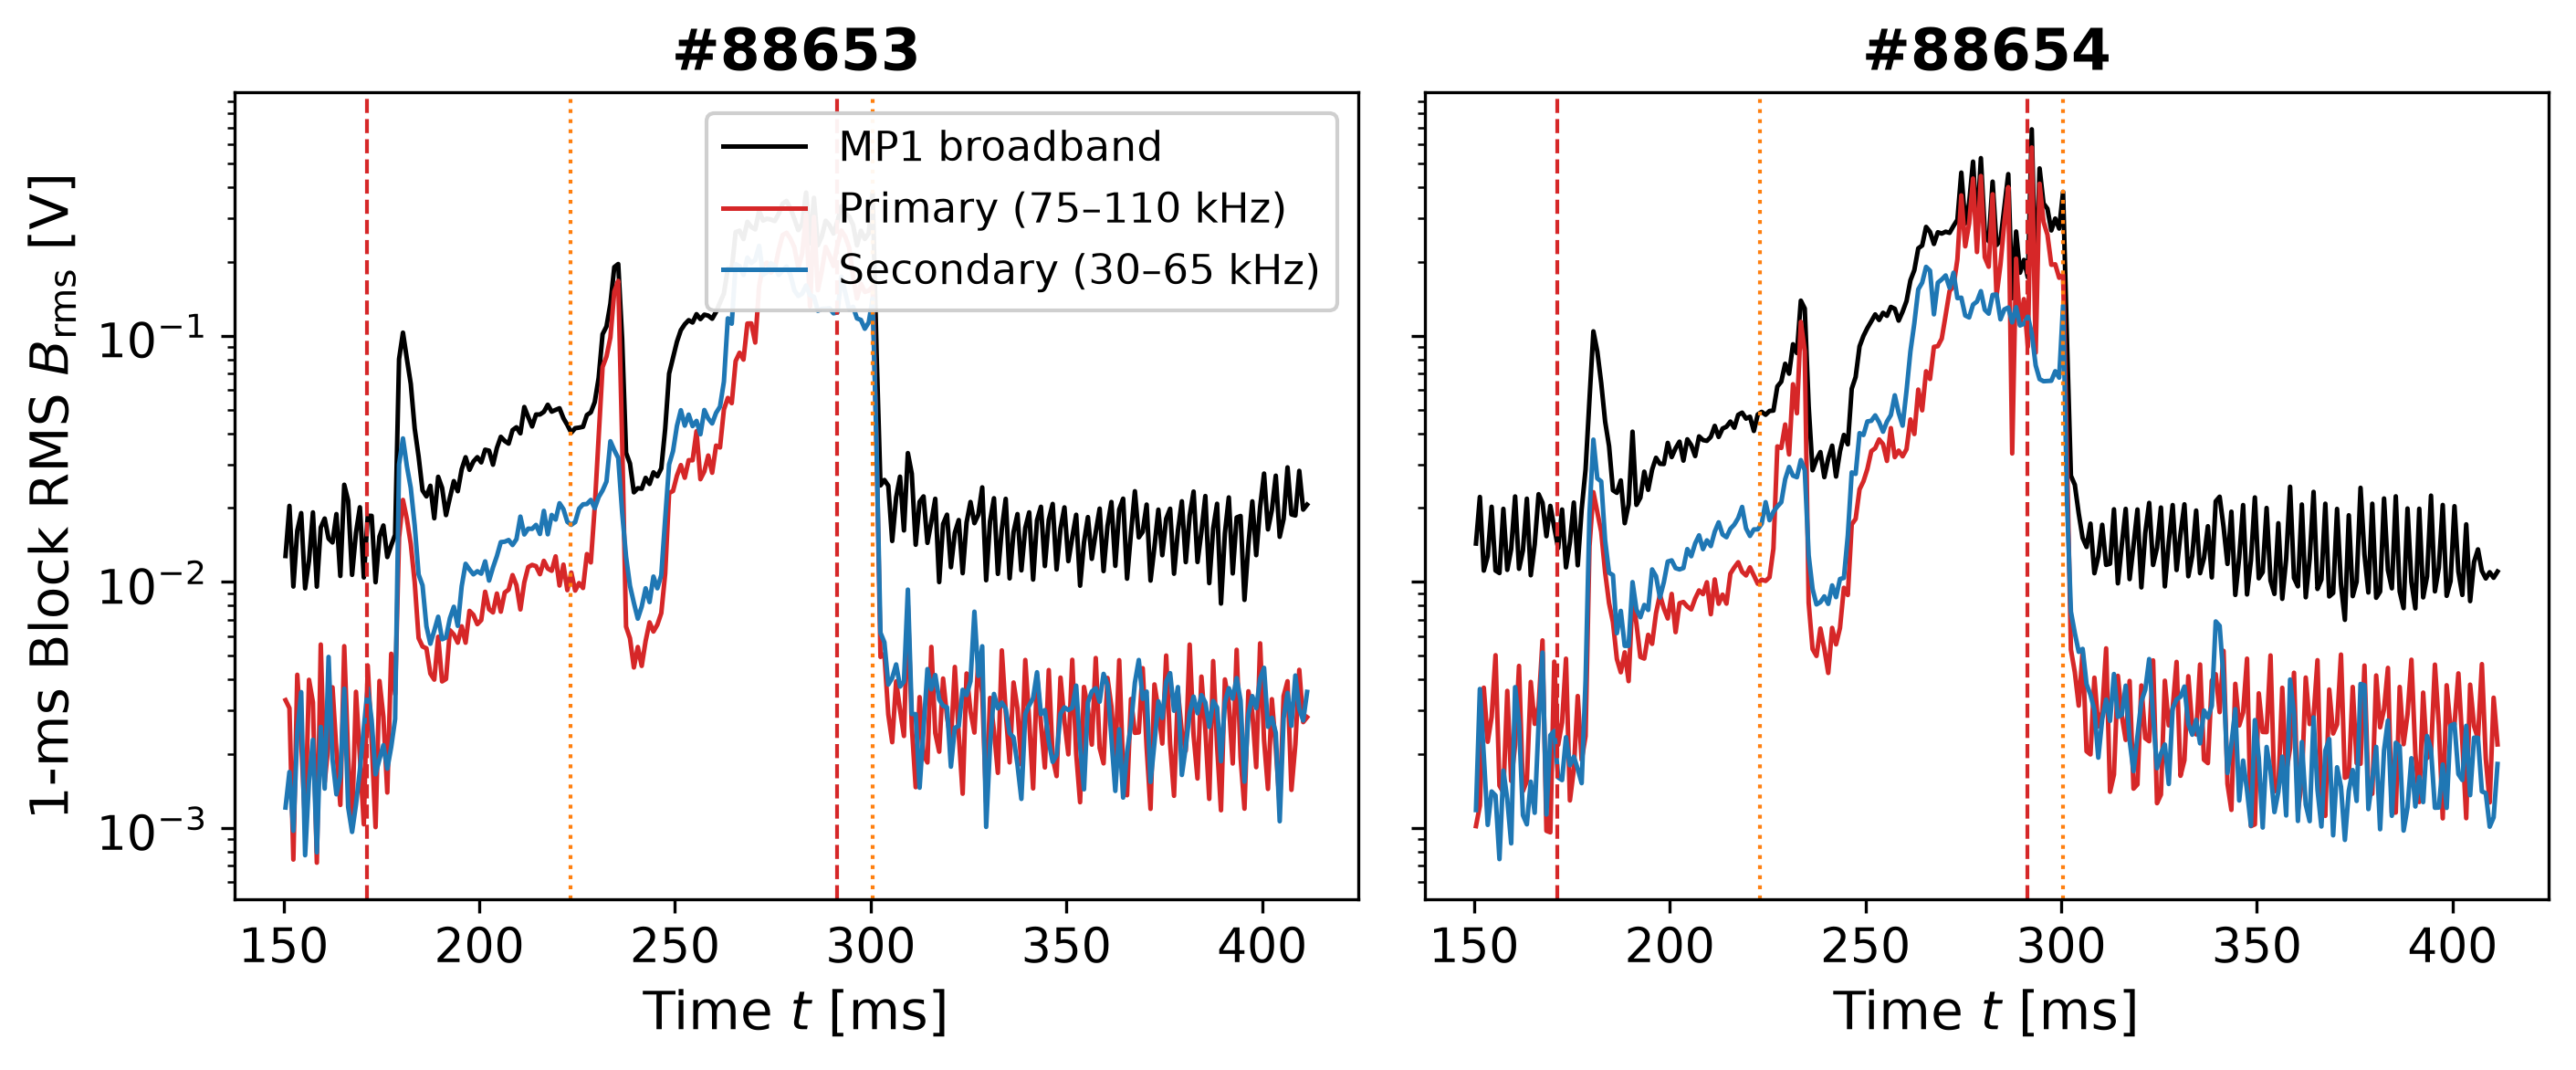
\includegraphics[width=0.90\textwidth]{Images/obj2_dynamics_and_structure/panels/fig_rms_vs_time_both_shots.png}
  \caption[MP1 RMS per millisecond, both shots]{Uncalibrated $1~\mathrm{ms}$-block MP1 RMS traces (log scale) across three frequency bands for \#88653 and \#88654.}
  \label{fig:rms_vs_time}
\end{figure}
Table~\ref{tab:discharge_phases} and Figures~\ref{fig:heating_timeline} and~\ref{fig:rms_vs_time} detailed discharge evolution across heating phases ($N = 1$ ECH-off transition per shot; vertical red and orange lines in Figure~\ref{fig:heating_timeline} marked the half-level ECH and NBIS10 crossings, where $291.2~\mathrm{ms}$ slightly preceded the $291.32~\mathrm{ms}$ \texttt{ECHRG500} half-drop). In shot \#88653, broadband MP1 RMS rose from $0.016~\mathrm{V}$ (pre-plasma) and $0.040~\mathrm{V}$ (ECH-only, $\gamma^2 = 0.158$) to $0.087~\mathrm{V}$ in early $\mathrm{ECH}+\mathrm{NBI}$ ($\gamma^2 = 0.931$; lines at $87.9, 139.6~\mathrm{kHz}$) and $0.274~\mathrm{V}$ in late $\mathrm{ECH}+\mathrm{NBI}$ ($\gamma^2 = 0.972$; lines at $40.0, 88.9~\mathrm{kHz}$). Amplitude peaked at $0.281~\mathrm{V}$ during $\mathrm{NBI}$-only ($\gamma^2 = 0.997$) before decaying to $0.054~\mathrm{V}$ post-heating. Both shots showed matching $1~\mathrm{ms}$ RMS traces (Figure~\ref{fig:rms_vs_time}: broadband along with Bessel-filtered $75\text{--}110~\mathrm{kHz}$ and $30\text{--}65~\mathrm{kHz}$ bands), including an \emph{unresolved} burst near $180~\mathrm{ms}$, a brief $235~\mathrm{ms}$ burst coinciding with an $I_p$ drop (Figure~\ref{fig:heating_timeline}), and sustained dual-band activity over $260\text{--}300.4~\mathrm{ms}$.

\begin{table}[H]
\centering
\small
\caption[Mode frequency shifts across ECH switch-off]{Mode frequency shifts across ECH switch-off.}
\label{tab:ech_switchoff_summary}
\sbox0{%
\begin{tabular}{lcccccccc}
\toprule
Quantity & \#88653 shift (kHz) & Sliding rank (-) & $p$ sliding (-) & Non-overlap rank (-) & $p$ non-overlap (-) & Surrogate $p$ (-) & \#88654 shift (kHz) & Same sign \\
\midrule
Secondary centroid & $-9.69$ & 0/54 & 0.018 & 0/5 & 0.167 & 0.004 & $-9.86$ & yes \\
Secondary dominant & $-10.74$ & 0/54 & 0.018 & 0/5 & 0.167 & 0.124 & $-12.70$ & yes \\
Primary centroid & $-3.94$ & 7/54 & 0.145 & 1/5 & 0.333 & 0.194 & $-8.55$ & yes \\
Primary dominant & $-5.86$ & 1/54 & 0.036 & 0/5 & 0.167 & 0.240 & $-11.72$ & yes \\
\bottomrule
\end{tabular}}
\ifdim\wd0>\textwidth\resizebox{\textwidth}{!}{\usebox0}\else\usebox0\fi
\par\smallskip{\footnotesize Two-sided rank $p$-values (500 surrogates for surrogate $p$); sliding placements overlap, whereas non-overlapping placements bound $p\ge 0.167$. One transition per shot.}
\end{table}
\begin{table}[H]
\centering
\small
\caption[Stored-energy slope change across ECH switch-off]{Stored-energy slope change across ECH switch-off.}
\label{tab:ech_wp_step}
\sbox0{%
\begin{tabular}{lcc}
\toprule
Fit window (ms) & \#88653 [95\,\% CI] (kW) & \#88654 [95\,\% CI] (kW) \\
\midrule
2 & $-54.3$ [$-61.6$, $-47.6$] & $-81.1$ [$-90.8$, $-71.3$] \\
5 & $-60.9$ [$-65.3$, $-56.9$] & $-68.3$ [$-79.0$, $-59.2$] \\
\bottomrule
\end{tabular}}
\ifdim\wd0>\textwidth\resizebox{\textwidth}{!}{\usebox0}\else\usebox0\fi
\par\smallskip{\footnotesize Post- minus pre-291.2~ms slope (negative: slower rise or faster decay of $W_p$; not absorbed gyrotron power); window-dependent; $95\,\%$ block-bootstrap confidence intervals (CI) in brackets. Post-ECH $n_e$ minimum in \#88653: $+0.40$~ms raw, $+0.36$~ms Savitzky--Golay smoothed (not evaluated for \#88654).}
\end{table}


\begin{figure}[H]
  \centering
  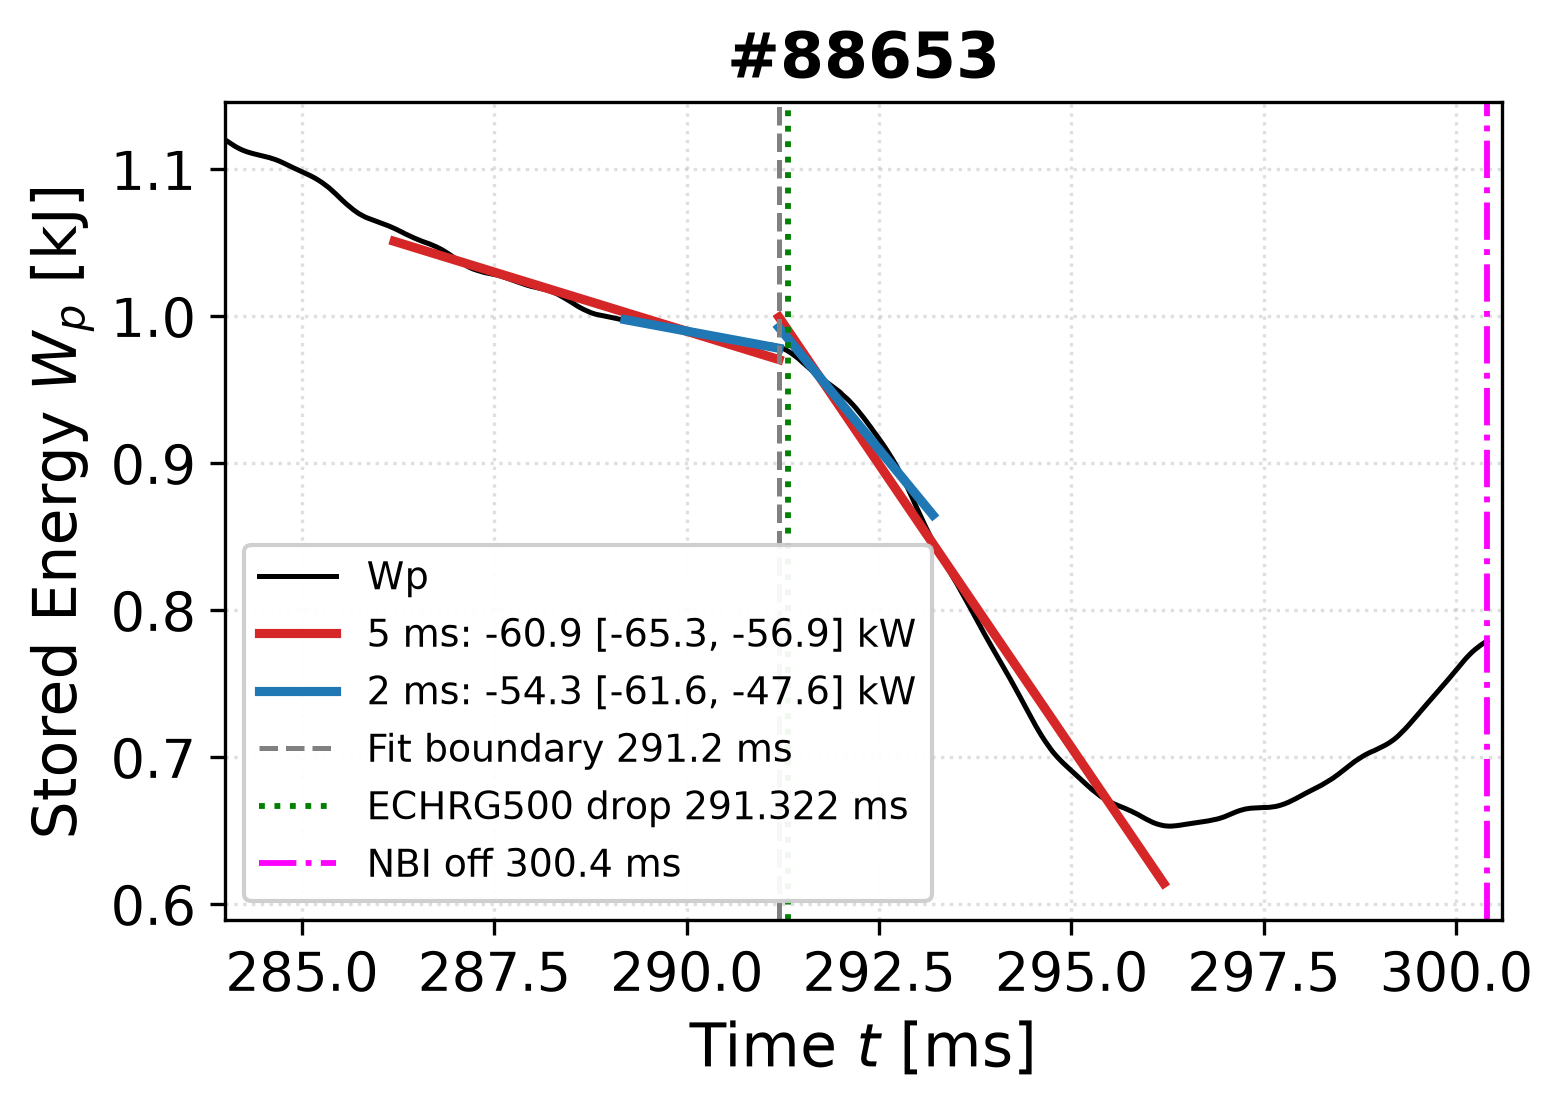
\includegraphics[width=0.49\textwidth]{Images/obj2_dynamics_and_structure/panels/fig_ech_wp_step_88653.png}
  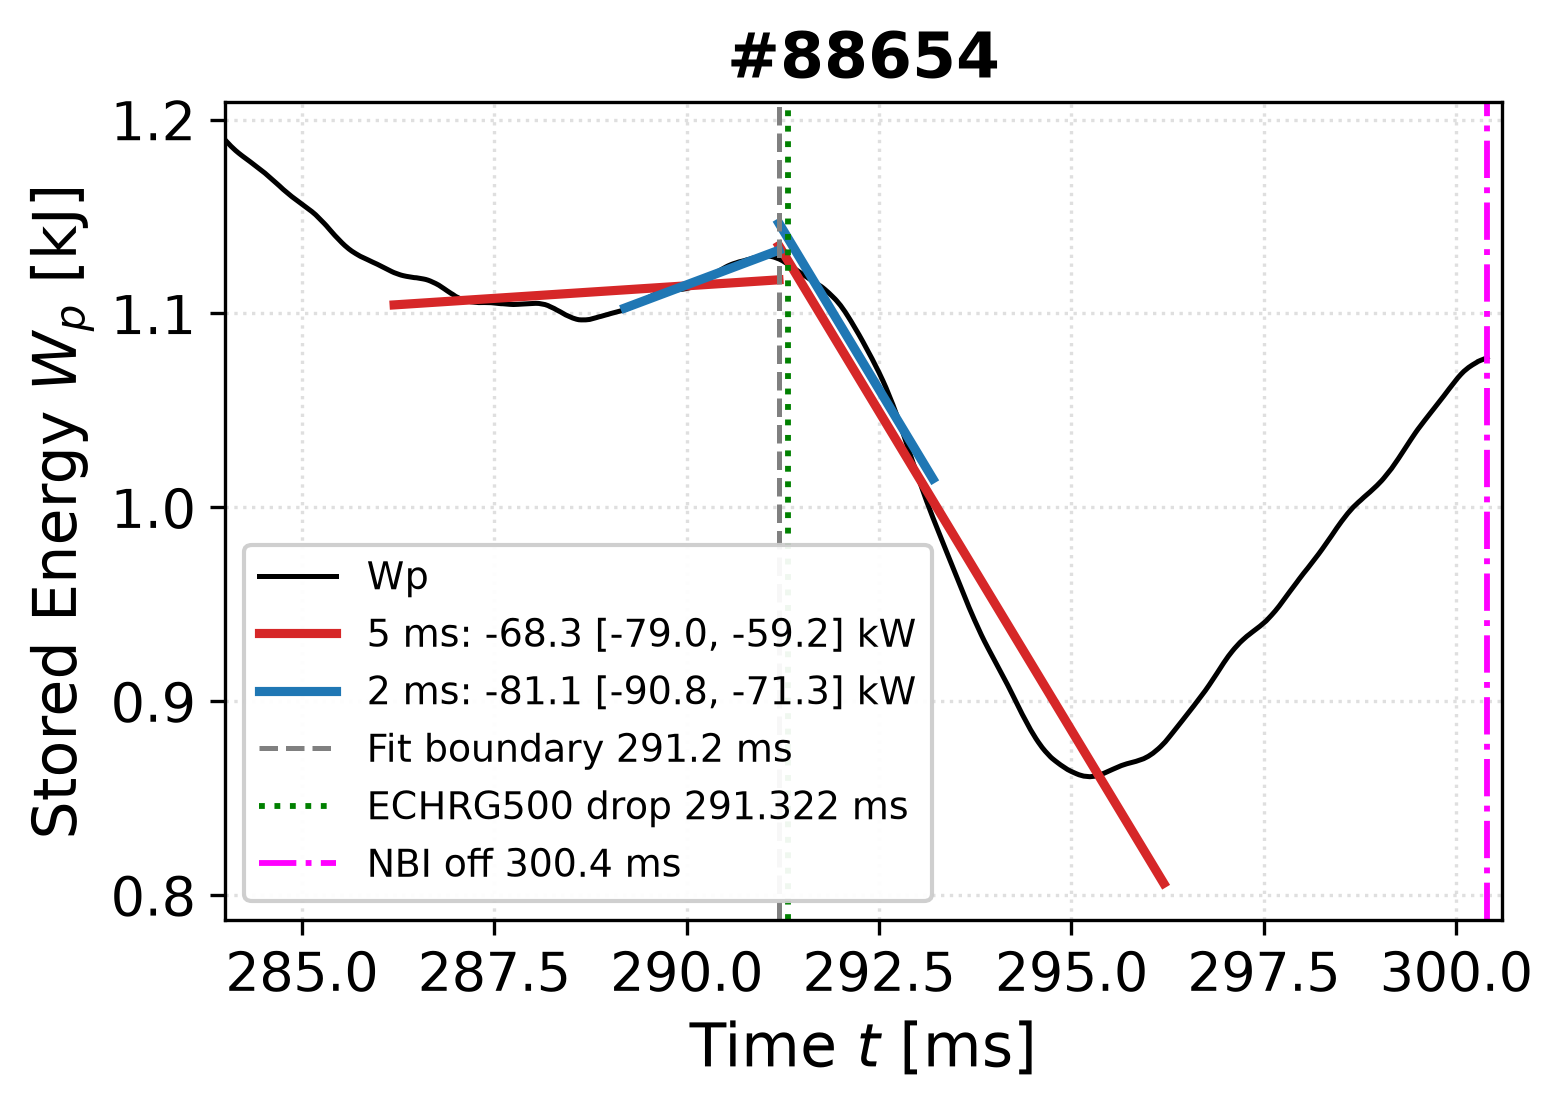
\includegraphics[width=0.49\textwidth]{Images/obj2_dynamics_and_structure/panels/fig_ech_wp_step_88654.png}
  \caption[Stored energy across ECH switch-off]{Stored energy $W_p$ across ECH switch-off ($291.2~\mathrm{ms}$) with $2$ and $5~\mathrm{ms}$ fits (\#88653, \#88654).}
  \label{fig:ech_wp_step}
\end{figure}

\begin{figure}[H]
  \centering
  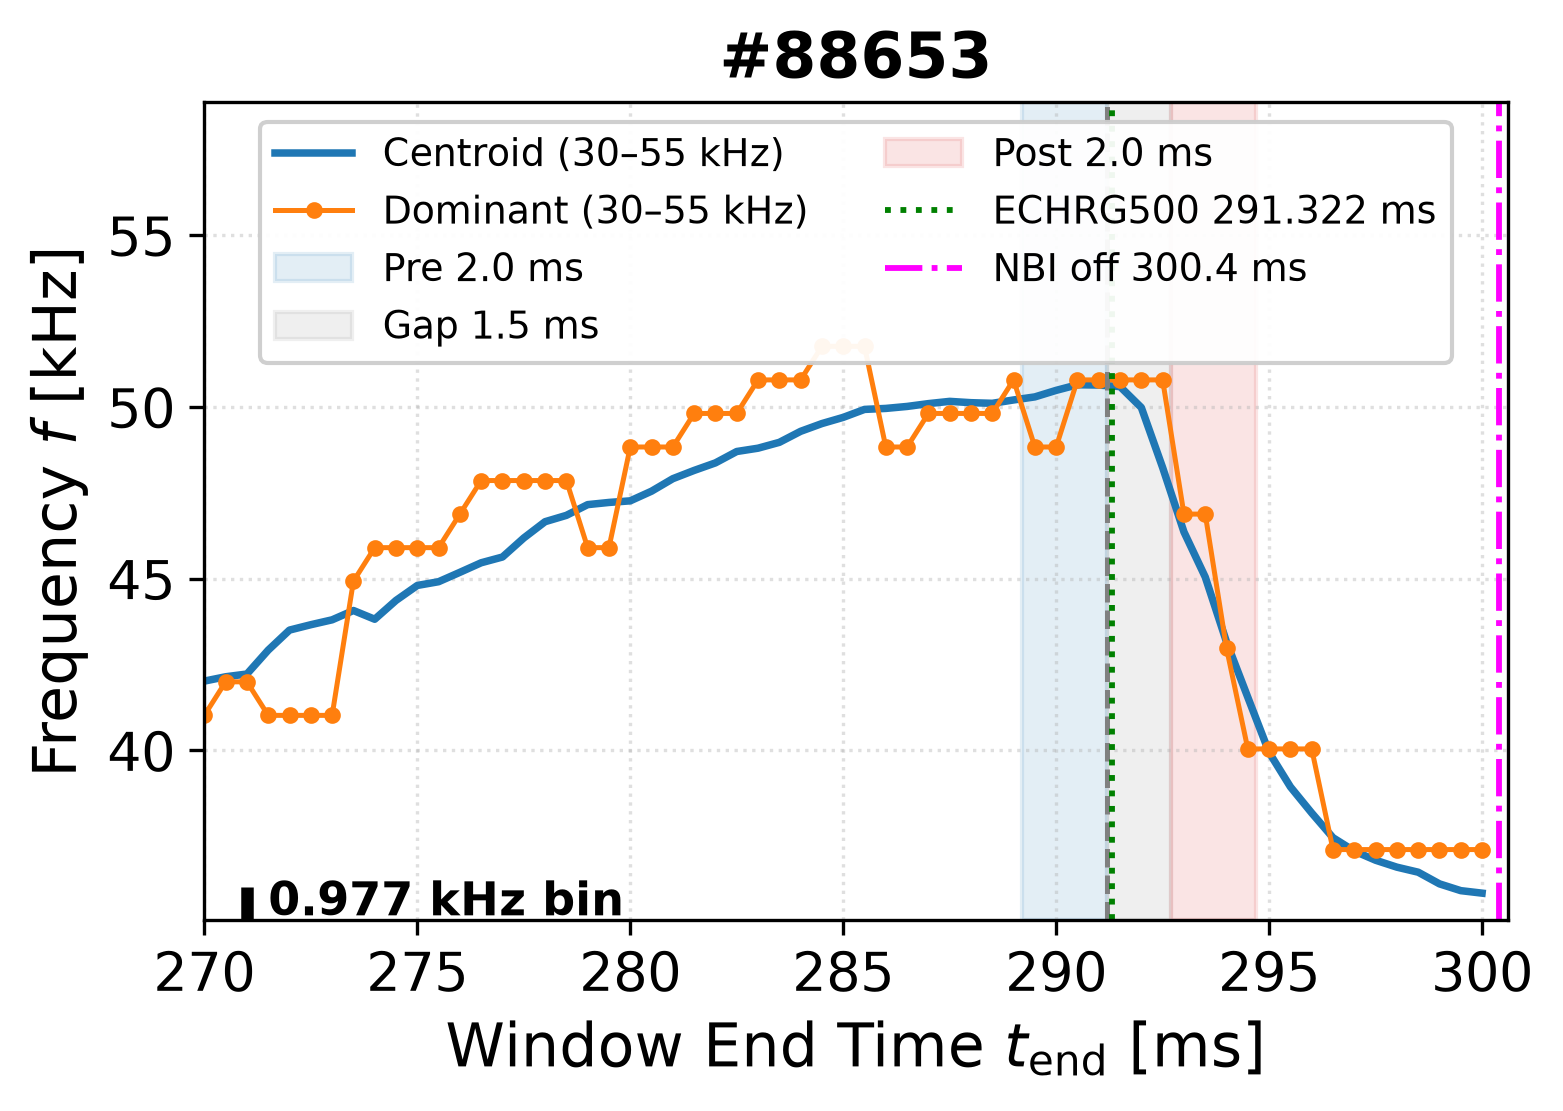
\includegraphics[width=0.49\textwidth]{Images/obj2_dynamics_and_structure/panels/fig_ech_secondary_freq_88653.png}
  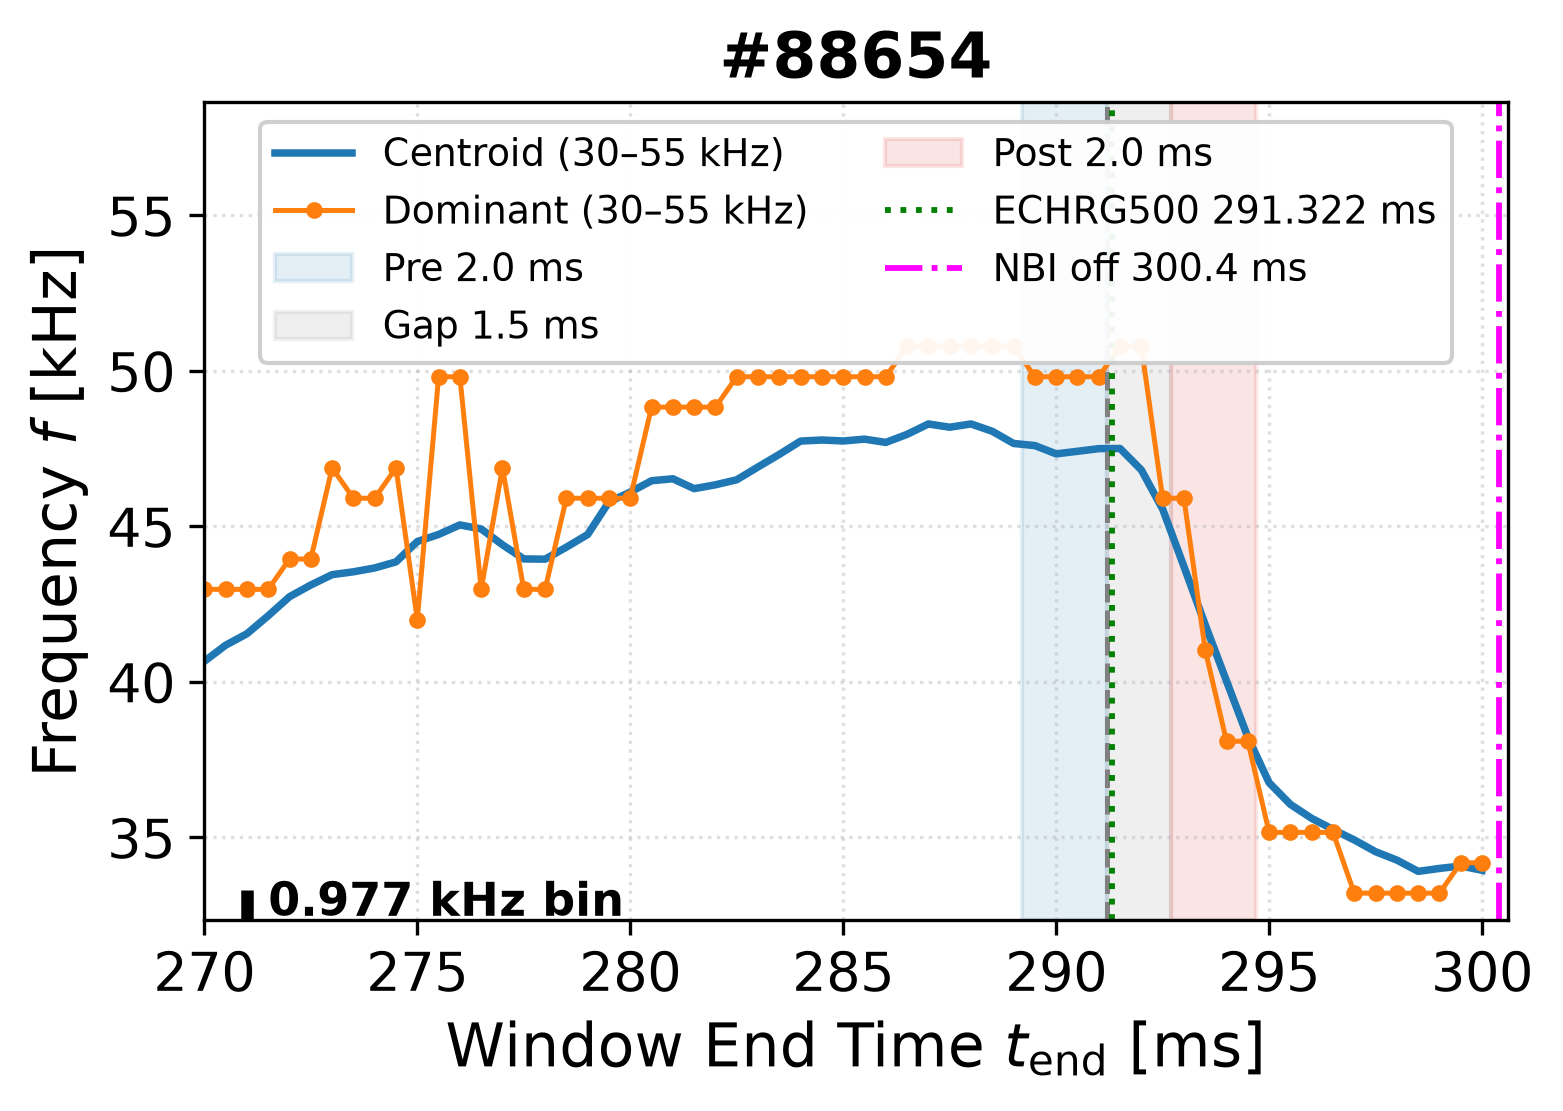
\includegraphics[width=0.49\textwidth]{Images/obj2_dynamics_and_structure/panels/fig_ech_secondary_freq_88654.png}
  \caption[Secondary-band frequency estimators]{Secondary-band ($30\text{--}55~\mathrm{kHz}$) centroid and dominant-bin frequencies across ECH switch-off for \#88653 and \#88654.}
  \label{fig:ech_secondary_freq}
\end{figure}
Tables~\ref{tab:ech_switchoff_summary} and~\ref{tab:ech_wp_step} and Figures~\ref{fig:ech_wp_step} and~\ref{fig:ech_secondary_freq} quantified the stored-energy slope change $\Delta(\mathrm{d}W_p/\mathrm{d}t)$ ($95~\%$ confidence interval, CI) and frequency shifts across $t_0 = 291.2~\mathrm{ms}$. In Figure~\ref{fig:ech_wp_step}, $\Delta(\mathrm{d}W_p/\mathrm{d}t)$ was negative and window-dependent in both shots: $-54.3~\mathrm{kW}$ ($[-61.6,\allowbreak -47.6]~\mathrm{kW}$ over $2~\mathrm{ms}$) and $-60.9~\mathrm{kW}$ ($[-65.3,\allowbreak -56.9]~\mathrm{kW}$ over $5~\mathrm{ms}$) in \#88653, versus $-81.1$ and $-68.3~\mathrm{kW}$ in \#88654. In \#88653, $n_e$ reached a local minimum $+0.40~\mathrm{ms}$ raw ($+0.36~\mathrm{ms}$ smoothed) after ECH-off. Physically, this $\mathrm{d}W_p/\mathrm{d}t$ step primarily reflected immediate removal of external ECH power at $t_0 = 291.2~\mathrm{ms}$ alongside any outward energy transport. In Figure~\ref{fig:ech_secondary_freq} (computed from trailing $2.0~\mathrm{ms}$ windows at $0.977~\mathrm{kHz}$ bins across shaded pre, $1.5~\mathrm{ms}$ gap, and post intervals) and Table~\ref{tab:ech_switchoff_summary}, the secondary centroid dropped by $-9.69~\mathrm{kHz}$ in \#88653 ($-9.86~\mathrm{kHz}$ in \#88654), exceeding all $54$ sliding ($p_{\mathrm{sliding}} = 0.018$) and $5$ non-overlapping ($p_{\mathrm{non\text{-}overlap}} \ge 0.167$) null placements with $p_{\mathrm{surr}} = 0.004$ (\emph{supported}). Because pre-transition upward chirping raised the baseline, this local $-9.69~\mathrm{kHz}$ step reconciled with the full-phase mean shift ($-6.1~\mathrm{kHz}$, Figure~\ref{fig:obj1_spectrogram}) and dominant peak step ($-7.8~\mathrm{kHz}$, Table~\ref{tab:mode_structure}). Discretized secondary peak shifts ($-10.74~\mathrm{kHz}$, $p_{\mathrm{surr}} = 0.124$) and primary-band shifts (centroid $-3.94~\mathrm{kHz}$, $p_{\mathrm{surr}} = 0.194$; dominant $-5.86~\mathrm{kHz}$, $p_{\mathrm{surr}} = 0.240$) remained \emph{inconclusive}. Moreover, a density-following fit ($f \propto n_e^{-\gamma}$ over $262\text{--}290$, $270\text{--}290$, and $275\text{--}291.2~\mathrm{ms}$) explained only $26.2~\%$, $21.3~\%$, and $17.8~\%$ of the drop, leaving the underlying mechanism \emph{unresolved}. This stronger sensitivity of the secondary band suggested a substantial $T_e$ or $\iota/2\pi$ role, consistent with ECH/ECCD tuning of core BAE and GAM frequencies~\cite{Varela2015,Varela2023,Yamamoto_2020,Zhong2024,Adulsiriswad_2024}.


\subsection[Objective 2 -- EPM-Heating Correlation and Statistical Metrics]{Objective 2 -- EPM-Heating Correlation\\ and Statistical Metrics}
\label{subsec:obj2}

\subsubsection{Envelope Correlations with \texorpdfstring{$I_p$, $W_p$, $n_e$}{Ip, Wp, ne}}
\label{subsubsec:obj2_envelope}

\begin{figure}[H]
  \centering
  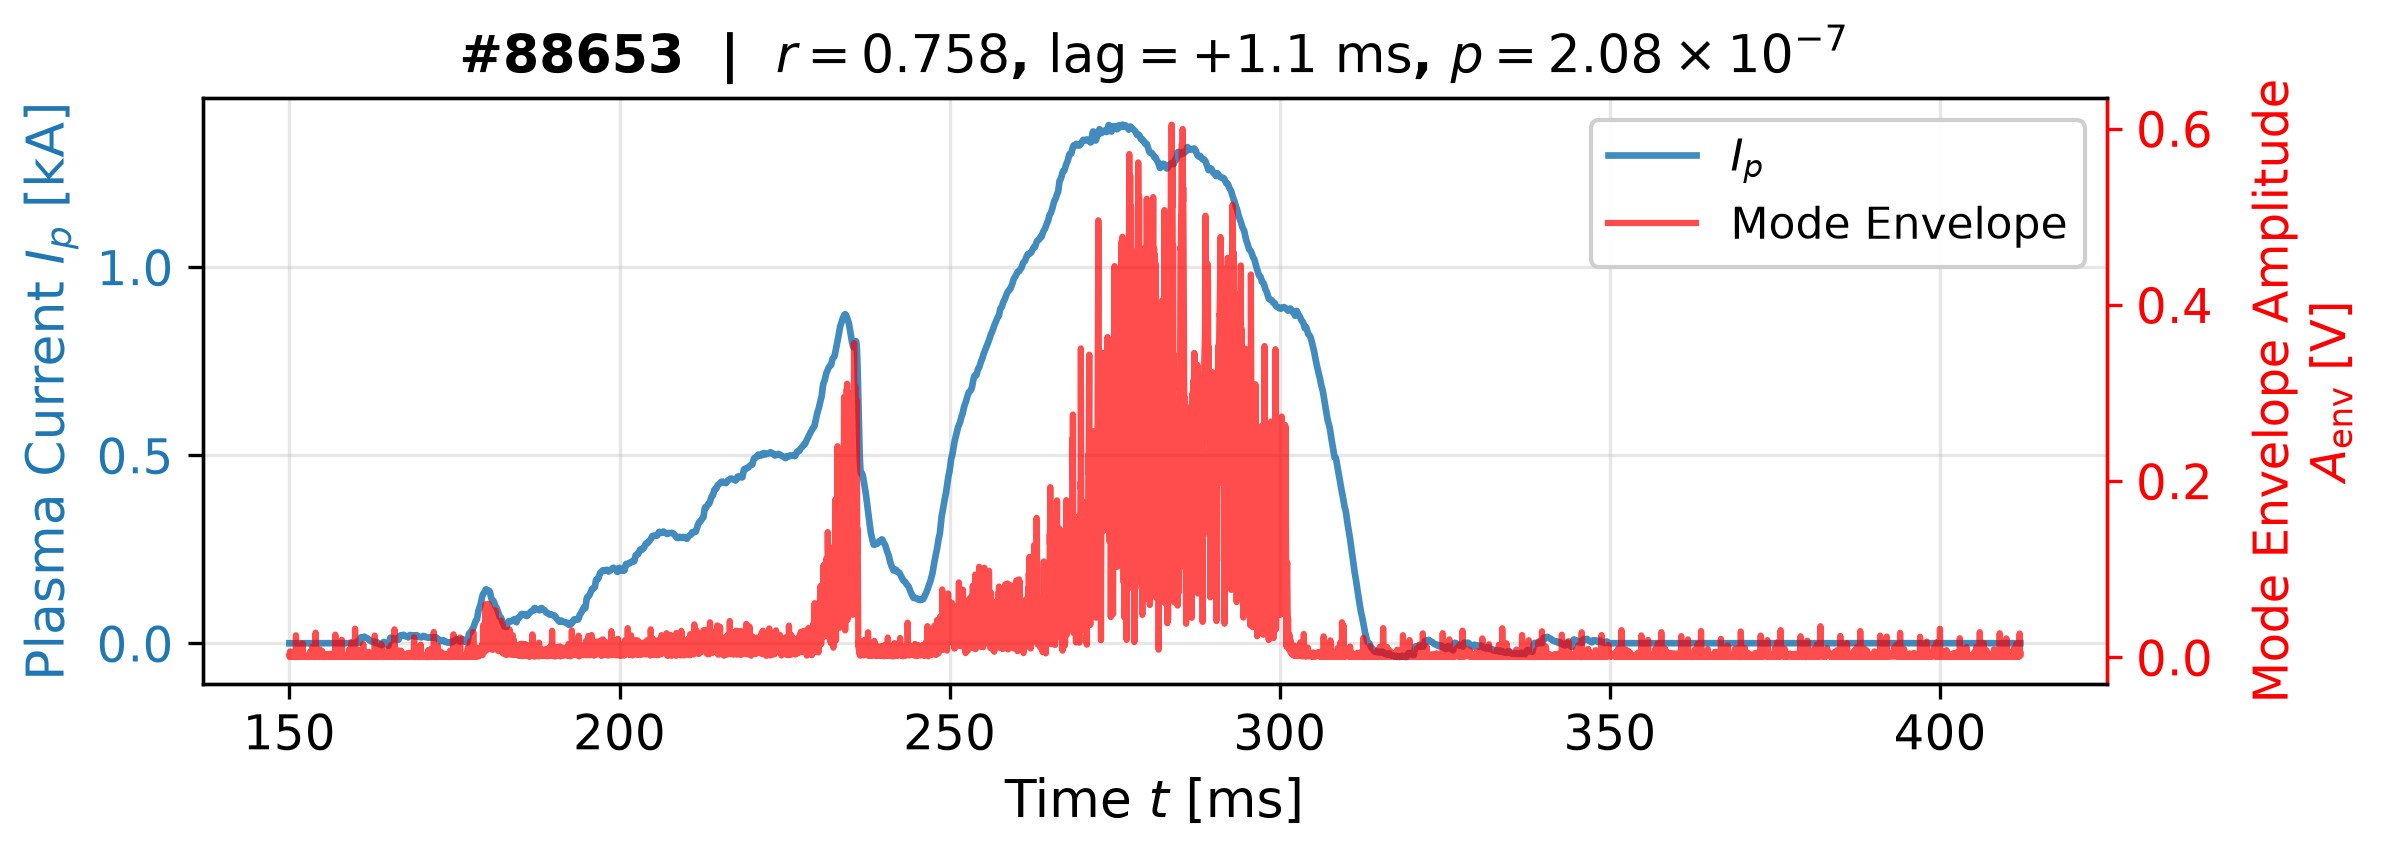
\includegraphics[width=0.86\textwidth]{Images/obj2_dynamics_and_structure/panels/mhd_analysis_objective2_88653_80_120kHz_panel1_correlation_plasma_current_ip15_vs_mode.png}
  \caption[Primary mode envelope correlation with plasma current]{Primary mode envelope ($80\text{--}120~\mathrm{kHz}$) versus plasma current $I_p$ over the full record (\#88653).}
  \label{fig:obj2_envelope_ip}
  \vspace{0.25em}
  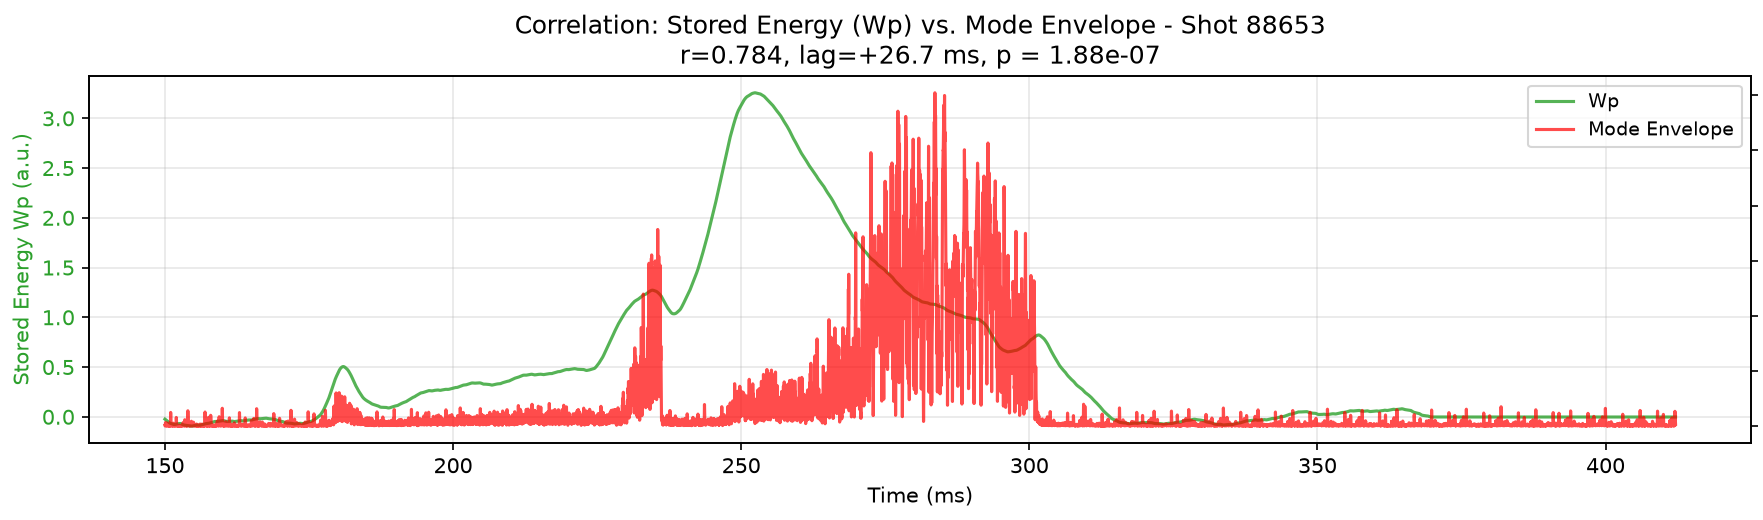
\includegraphics[width=0.86\textwidth]{Images/obj2_dynamics_and_structure/panels/mhd_analysis_objective2_88653_80_120kHz_panel2_correlation_stored_energy_wp_vs_mode_env.png}
  \caption[Primary mode envelope correlation with stored energy]{Primary mode envelope ($80\text{--}120~\mathrm{kHz}$) versus stored energy $W_p$ over the full record (\#88653).}
  \label{fig:obj2_envelope_wp}
  \vspace{0.25em}
  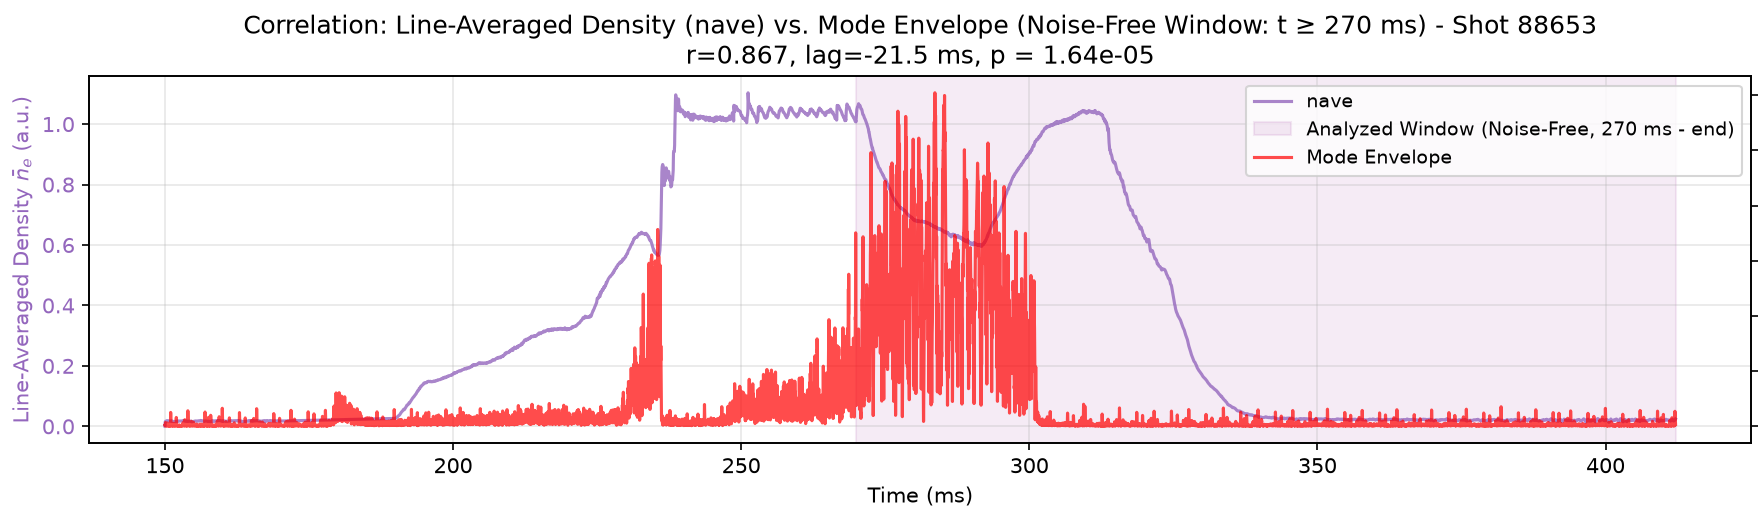
\includegraphics[width=0.86\textwidth]{Images/obj2_dynamics_and_structure/panels/mhd_analysis_objective2_88653_80_120kHz_panel3_correlation_line_averaged_density_nave_v.png}
  \caption[Primary mode envelope correlation with electron density]{Primary mode envelope ($80\text{--}120~\mathrm{kHz}$) versus line-averaged density $n_e$ ($t \geq 270.0~\mathrm{ms}$, \#88653).}
  \label{fig:obj2_envelope_ne}
\end{figure}
Figures~\ref{fig:obj2_envelope_ip}, \ref{fig:obj2_envelope_wp}, and~\ref{fig:obj2_envelope_ne} and Table~\ref{tab:obj2_both_shots} reported lagged cross-correlations of the $80\text{--}120~\mathrm{kHz}$ primary-mode envelope against $I_p$, $W_p$, and $n_e$. In shot \#88653, all three proxies exceeded $|r| > 0.70$. Specifically, $I_p$ yielded $r = 0.7575$ at lag $+1.10~\mathrm{ms}$ ($N_{\mathrm{eff}} = 34.1$, $p = 2.08 \times 10^{-7}$), and $W_p$ yielded $r = 0.7840$ at $+26.70~\mathrm{ms}$ after the $252~\mathrm{ms}$ peak ($N_{\mathrm{eff}} = 30.9$, $p = 1.88 \times 10^{-7}$). Over $t \ge 270~\mathrm{ms}$, $n_e$ yielded $r = 0.8666$ at lag $-21.50~\mathrm{ms}$ ($N_{\mathrm{eff}} = 15.8$, $p = 1.64 \times 10^{-5}$). Replicate shot \#88654 matched all lag directions ($+1.30$, $+28.90$, $-21.20~\mathrm{ms}$), with $n_e$ clearing threshold ($r = 0.7099$, $N_{\mathrm{eff}} = 22.9$) while $I_p$ ($0.6555$) and $W_p$ ($0.6590$) stayed below $0.70$. Because these traces shared heating ramps and collapsed to near-zero partial correlation under ECH-step control ($r = +0.0609, +0.0023$ for envelope; $+0.076, -0.074$ for frequency), macroscopic correlations remained \emph{suggestive} rather than causal.

\begin{table}[H]
\centering
\footnotesize
\setlength{\tabcolsep}{4pt}
\renewcommand{\arraystretch}{1.15}
\caption[Primary-mode correlations and scaling models for both shots]{Primary-mode correlations and scaling models for both shots.}
\label{tab:obj2_both_shots}
\begin{tabular}{lcccccccc}
\toprule
 & \multicolumn{4}{c}{\#88653} & \multicolumn{4}{c}{\#88654} \\
\cmidrule(lr){2-5}\cmidrule(lr){6-9}
Quantity & \shortstack{Pearson\\$r$ (-)} & $N_{\rm eff}$ (-) & \shortstack{Lag\\(ms)} & $p$ (-) & \shortstack{Pearson\\$r$ (-)} & $N_{\rm eff}$ (-) & \shortstack{Lag\\(ms)} & $p$ (-) \\
\midrule
$I_p$ & 0.7575 & 34.1 & $+1.10$ & $2.08\times10^{-7}$ & 0.6555 & 46.8 & $+1.30$ & $6.10\times10^{-7}$ \\
$W_p$ & 0.7840 & 30.9 & $+26.70$ & $1.88\times10^{-7}$ & 0.6590 & 42.3 & $+28.90$ & $1.89\times10^{-6}$ \\
\shortstack[l]{$n_e$ (270 ms\\to end)} & 0.8666 & 15.8 & $-21.50$ & $1.64\times10^{-5}$ & 0.7099 & 22.9 & $-21.20$ & $1.55\times10^{-4}$ \\
\midrule
\multicolumn{9}{l}{\textbf{Candidate Frequency Scaling Models (Best Fit in Burst Window)}} \\
\midrule
\shortstack[l]{Primary best\\scaling $r$} & \multicolumn{4}{c}{\shortstack{BAE Coupled ($\sqrt{v_A^2 + c_s^2}$):\\$+0.545$ ($p_{\mathrm{adj}}=0.139$)}} & \multicolumn{4}{c}{\shortstack{Stored Energy ($W_p$):\\$+0.604$ ($p_{\mathrm{adj}}=0.099$)}} \\
\shortstack[l]{Secondary best\\scaling $r$} & \multicolumn{4}{c}{\shortstack{BAE Acoustic ($\sqrt{T_e}$):\\$+0.848$ ($p_{\mathrm{adj}}=0.162$)}} & \multicolumn{4}{c}{\shortstack{Stored Energy ($W_p$):\\$+0.343$ ($p_{\mathrm{adj}}=0.157$)}} \\
\midrule
\multicolumn{9}{l}{\textbf{ECH-Step-Controlled Partial Correlations}} \\
\midrule
\shortstack[l]{Envelope, ECH-step-\\controlled $r$} & \multicolumn{4}{c}{$+0.0609$} & \multicolumn{4}{c}{$+0.0023$} \\
\shortstack[l]{Frequency, ECH-step-\\controlled $r$} & \multicolumn{4}{c}{$+0.076$} & \multicolumn{4}{c}{$-0.074$} \\
\bottomrule
\end{tabular}
\par\smallskip Primary band ($80\text{--}120$~kHz) correlations evaluated per discharge (\#88654 serves as an independent same-direction check); secondary band ($40\text{--}80$~kHz) best scaling models are listed alongside primary scaling for completeness. Lag denotes peak cross-correlation offset; $p$-values use autocorrelation-adjusted $N_{\rm eff}$. Correlations remain \emph{suggestive} at most due to shared heating ramps and limited $N_{\rm eff}$.
\end{table}


\subsubsection{Verification of Relative \texorpdfstring{$T_e$}{Te} Proxy and Frequency Scaling Models}
\label{subsubsec:obj2_scaling}

To test whether low-pass filtered ECE traces followed slow thermal evolution, baseline-subtracted non-saturated channels were filtered with a 4th-order zero-phase Butterworth LPF ($f_c = 30~\mathrm{Hz}$ SOS), removing ${\sim}800~\mathrm{Hz}$ sawtooth and MHD modulations. Figure~\ref{fig:ece_te_verification}(a) compared these normalized $30~\mathrm{Hz}$ low-pass ECE signals (\texttt{ECE12FAST} and \texttt{ECE9FAST}) against stored energy $W_p(t)$, line-averaged density $n_e(t)$, and the diamagnetic temperature proxy $T_{e,\mathrm{dia}} \propto W_p/n_e$ over $240.0\text{--}305.0~\mathrm{ms}$ across density pump-out ($270.0\text{--}291.2~\mathrm{ms}$) and ECH shut-off ($291.2~\mathrm{ms}$).

\begin{figure}[H]
  \centering
  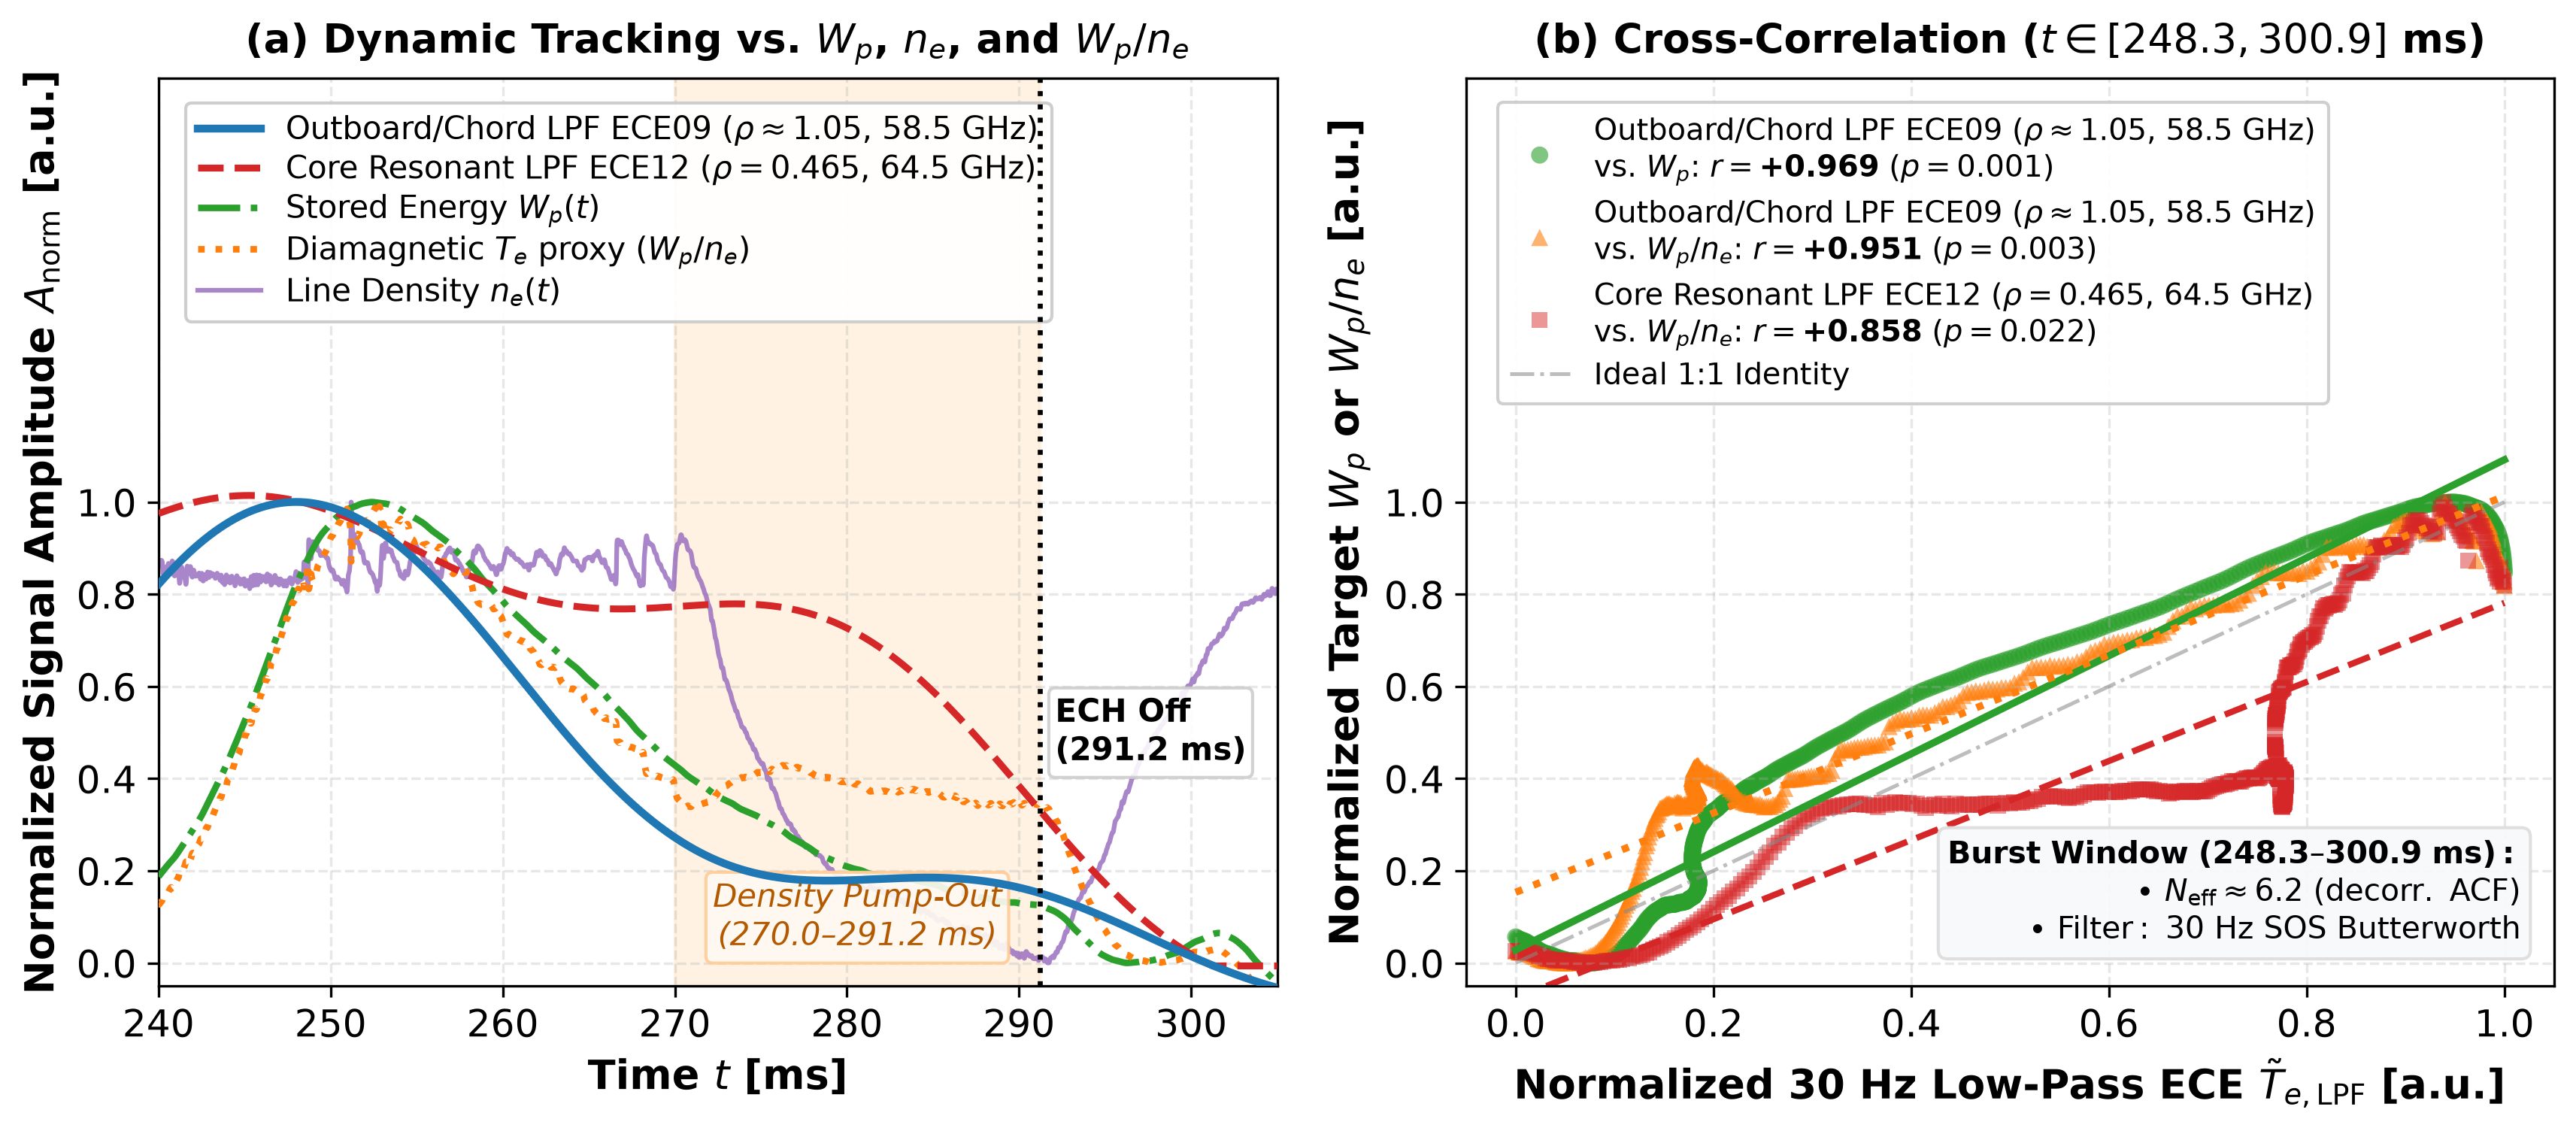
\includegraphics[width=0.98\textwidth]{Images/obj2_dynamics_and_structure/mhd_ece_lpf_te_verification_88653.png}
  \caption[Verification of relative $T_e$ proxy via low-pass filtered ECE]{Verification of relative $T_e$ proxy in shot \#88653: (a)~normalized $30~\mathrm{Hz}$ low-pass ECE traces and (b)~burst-window regressions.}
  \label{fig:ece_te_verification}
\end{figure}

Within the active burst window ($248.3\text{--}300.9~\mathrm{ms}$, Figure~\ref{fig:ece_te_verification}(b)), the optically thick resonant core channel \texttt{ECE12FAST} ($64.5~\mathrm{GHz}$, $\rho = 0.465$) served as the localized core thermal proxy, tracking both $W_p/n_e$ ($r = +0.858$, $p = 0.022$) and $W_p$ ($r = +0.811$). By contrast, \texttt{ECE9FAST} ($58.5~\mathrm{GHz}$, $\rho \approx 1.05$) represented a non-saturated outboard boundary / chord-integrated radiometer channel rather than a localized core measurement. Its $30~\mathrm{Hz}$ low-pass filtered intensity nonetheless tracked global stored energy $W_p$ ($r = +0.969$, $p = 0.001$, $N_{\mathrm{eff}} \approx 6.2$; $r = +0.805$ full shot) and $W_p/n_e$ ($r = +0.951$, $p = 0.003$). This reflected optically thin X2 emission capturing wall-reflected and chord-averaged bulk plasma behavior. Within the modest effective sample size ($N_{\mathrm{eff}} \approx 6.2$), this quantitative consistency supported $30~\mathrm{Hz}$ low-pass filtered ECE as a relative thermal evolution proxy.

\begin{figure}[H]
  \centering
  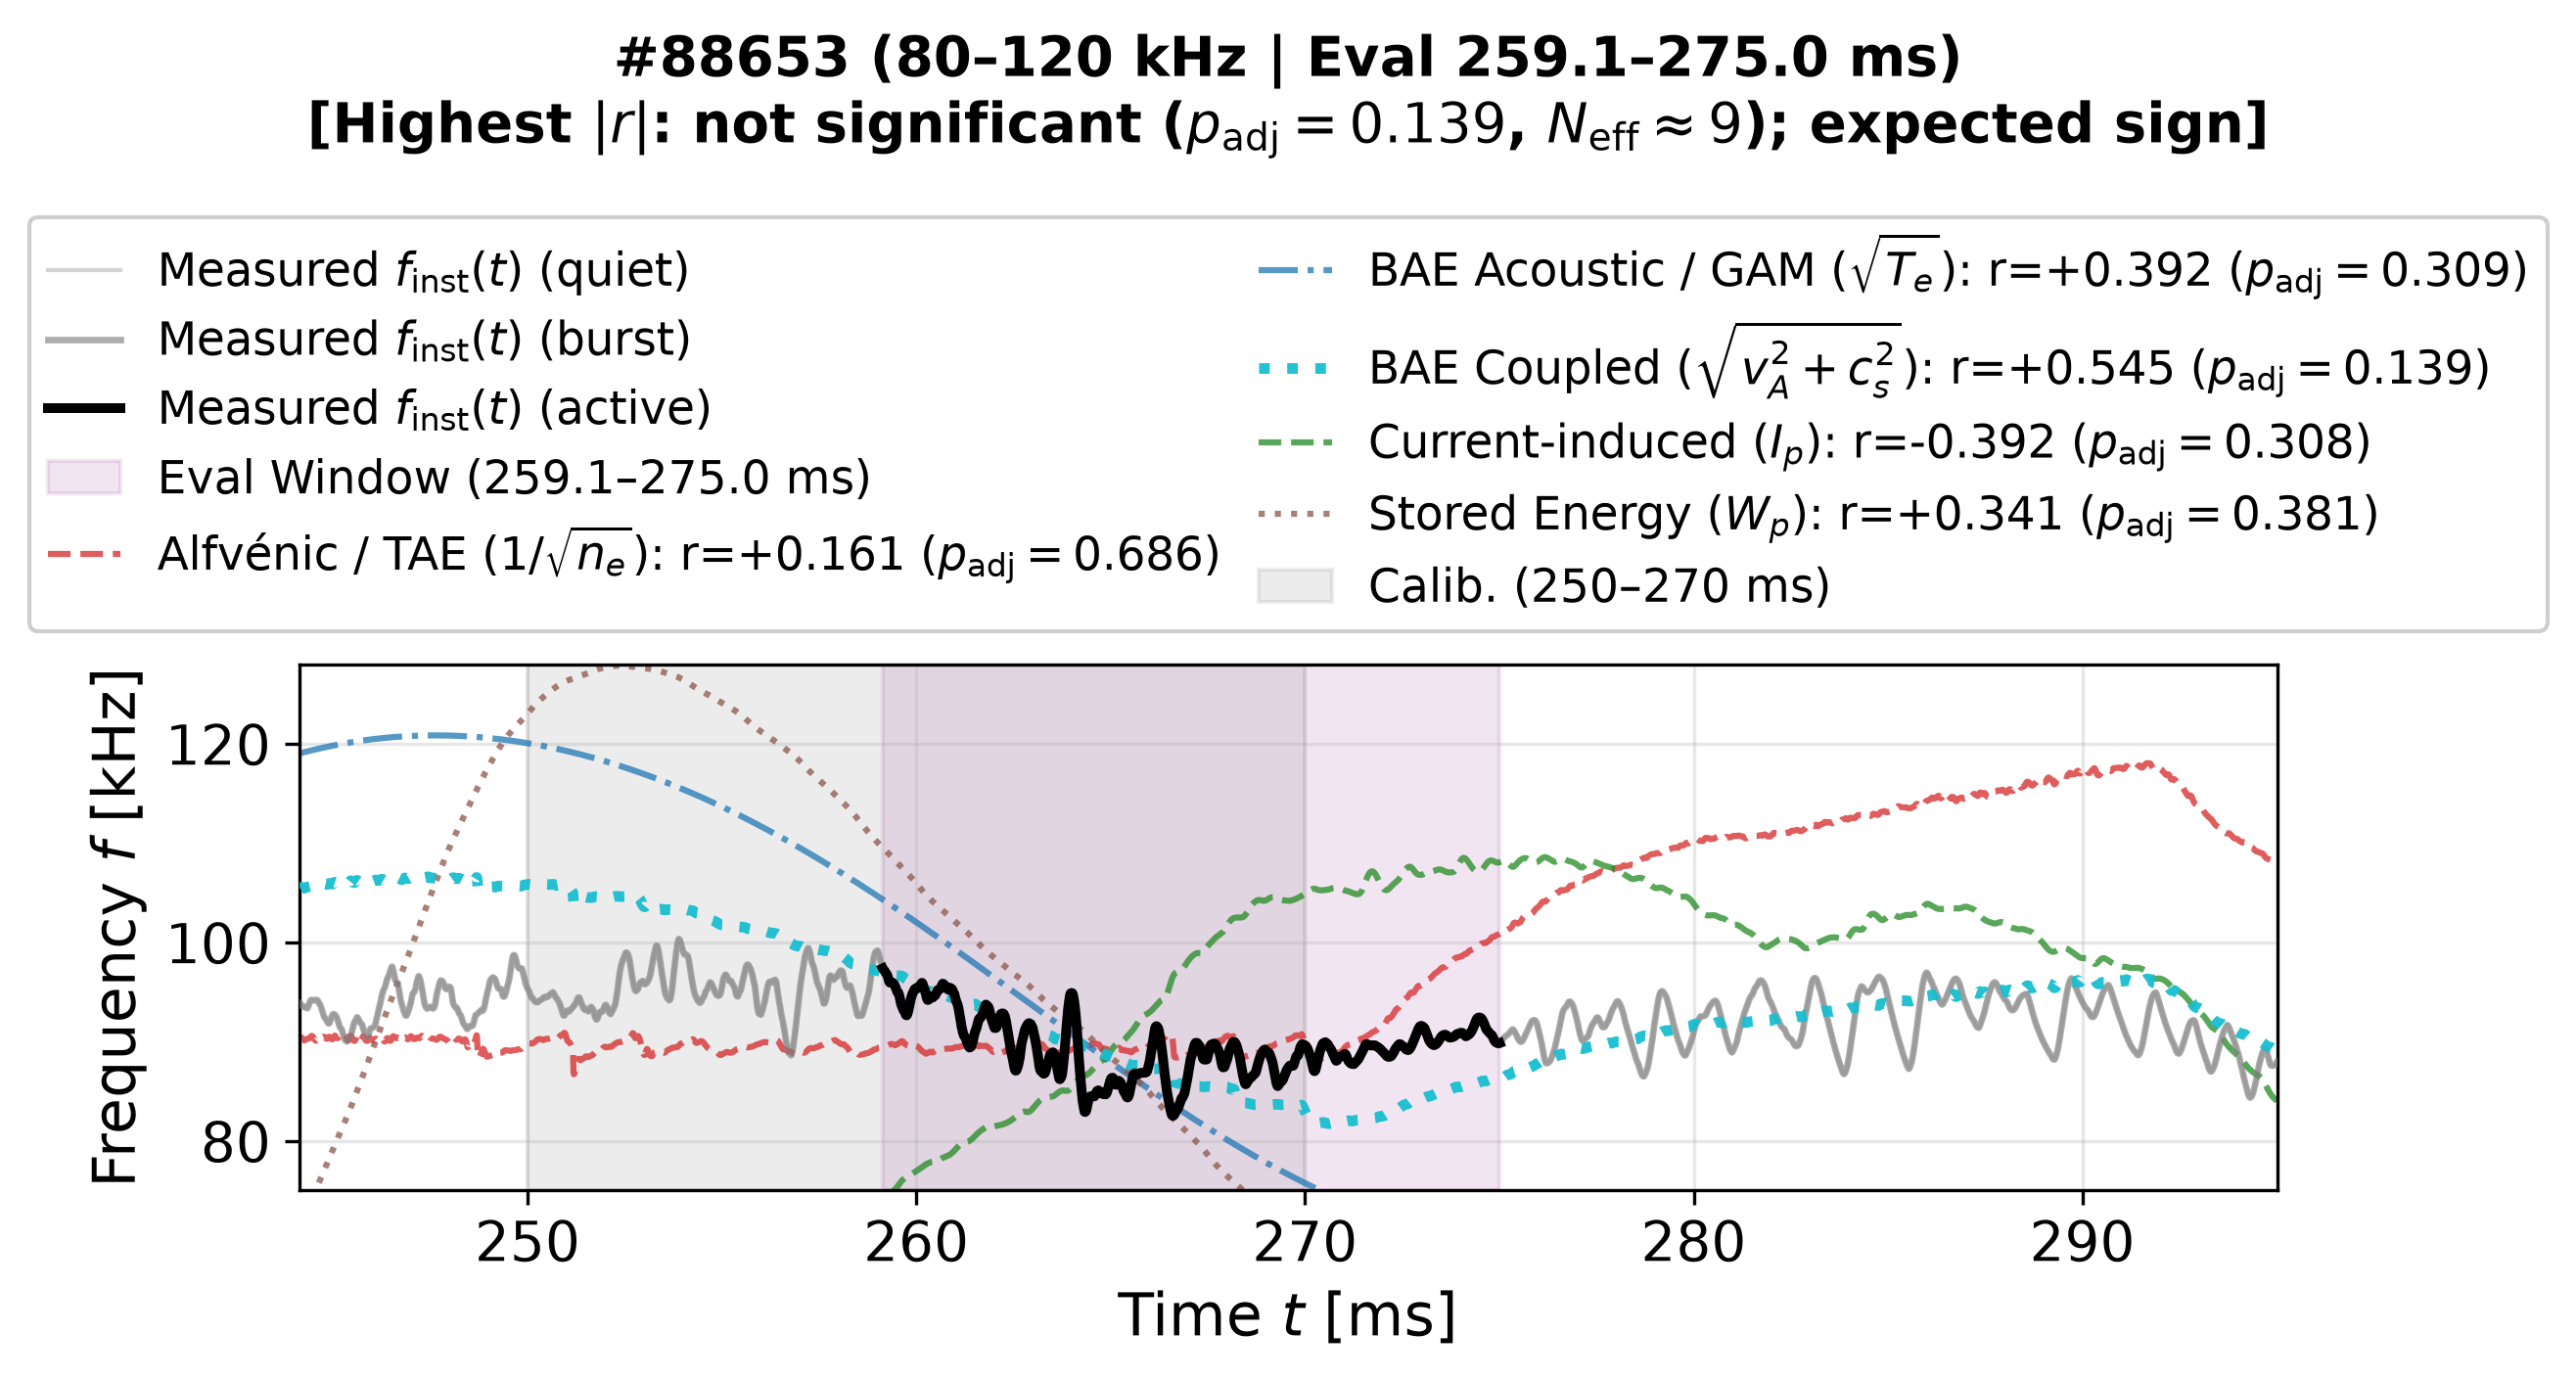
\includegraphics[width=0.92\textwidth]{Images/obj2_dynamics_and_structure/panels/mhd_analysis_objective2_heating_88653_80_120kHz_panel4_energetic_particle_mode_identification_m.png}
  \caption[Primary mode frequency response to candidate scaling models]{Primary mode ($80\text{--}120~\mathrm{kHz}$) frequency versus $30~\mathrm{Hz}$ LPF scaling models ($259.1\text{--}275.0~\mathrm{ms}$, \#88653).}
  \label{fig:obj2_epm_models_primary}
  \vspace{0.3em}
  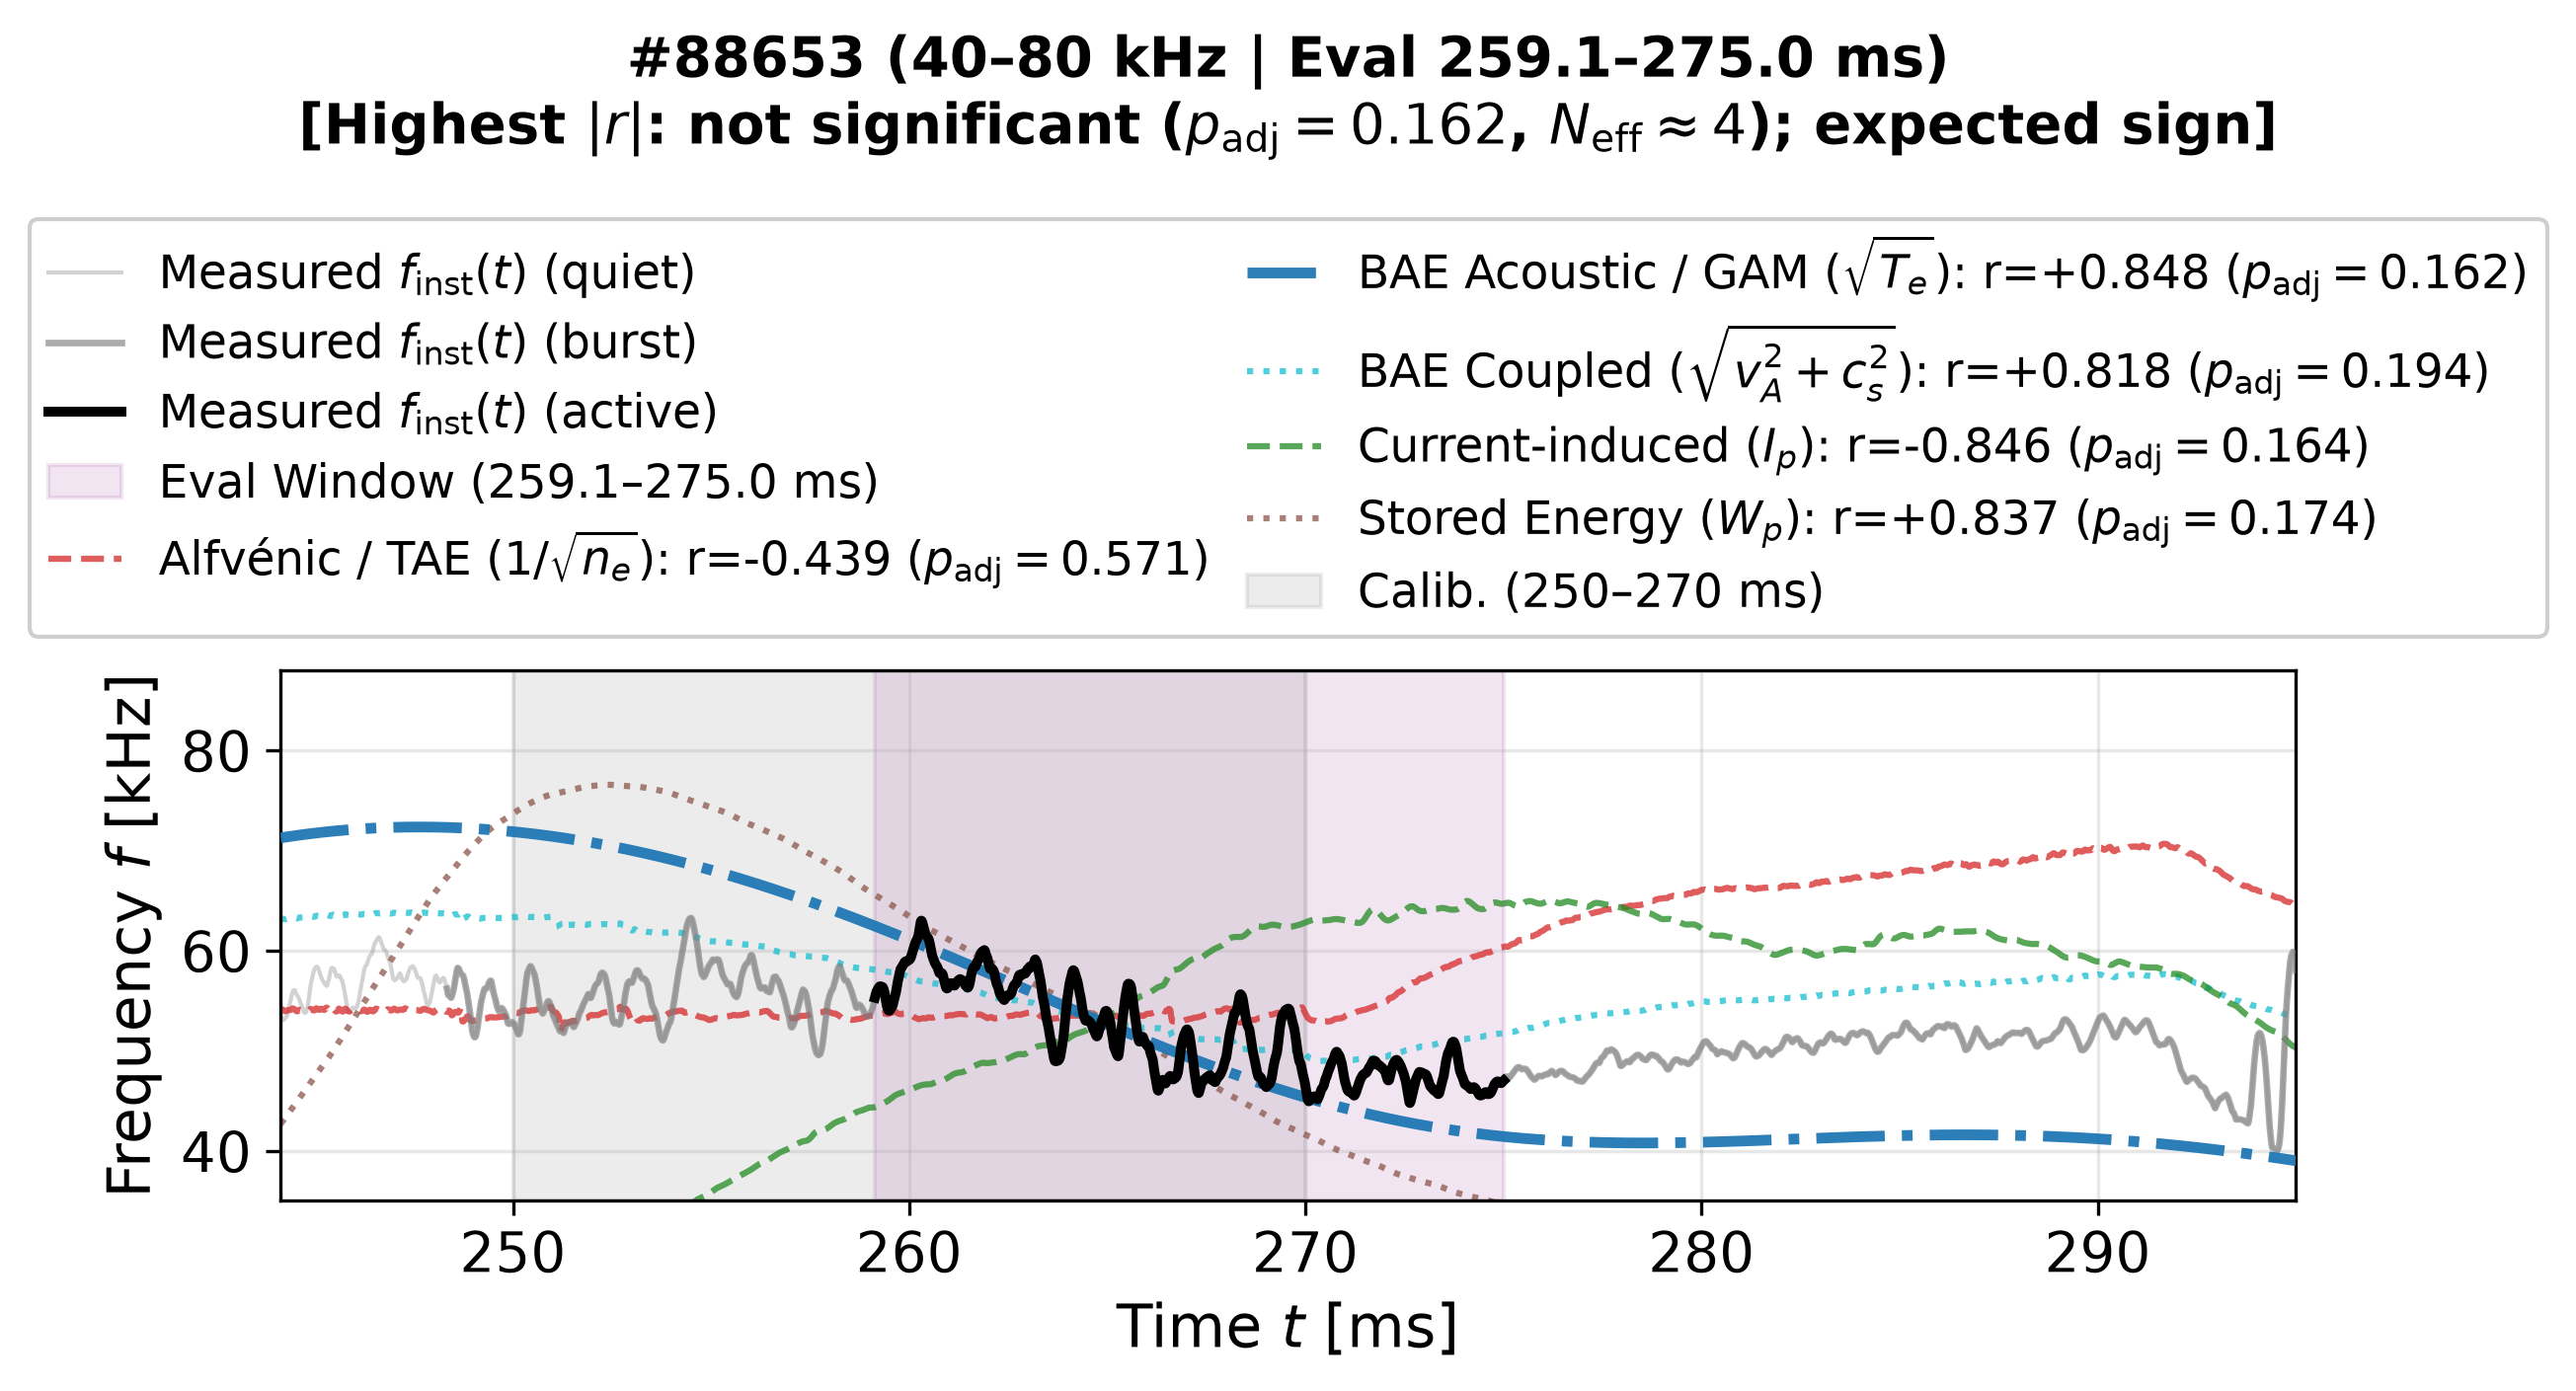
\includegraphics[width=0.92\textwidth]{Images/obj2_dynamics_and_structure/panels/mhd_analysis_objective2_heating_88653_40_80kHz_panel4_energetic_particle_mode_identification_m.png}
  \caption[Secondary mode frequency response to candidate scaling models]{Secondary mode ($40\text{--}80~\mathrm{kHz}$) frequency versus $30~\mathrm{Hz}$ LPF scaling models ($259.1\text{--}275.0~\mathrm{ms}$, \#88653).}
  \label{fig:obj2_epm_models_secondary}
\end{figure}

Figures~\ref{fig:obj2_epm_models_primary} and~\ref{fig:obj2_epm_models_secondary} compared primary ($80\text{--}120~\mathrm{kHz}$) and secondary ($40\text{--}80~\mathrm{kHz}$) frequency evolution in \#88653 against the five time-varying scaling models (calibrated on $250.0\text{--}270.0~\mathrm{ms}$) evaluated over $259.1\text{--}275.0~\mathrm{ms}$. Flat-top NBI beam scalings remained constant across this interval, while BAE traces used $30~\mathrm{Hz}$ SOS LPF smoothing. Filtering out ${\sim}800~\mathrm{Hz}$ sawtooth noise prevented sign-inversion artifacts and yielded positive acoustic tendencies for the primary mode: BAE Coupled ($\sqrt{v_A^2+c_s^2}$, $r = +0.545$, $p_{\mathrm{adj}} = 0.139$, $N_{\mathrm{eff}} \approx 9$) and BAE Acoustic ($\sqrt{T_e}$, $r = +0.392$, $p_{\mathrm{adj}} = 0.309$). In the secondary band, BAE Acoustic ranked highest ($r = +0.848$, $p_{\mathrm{adj}} = 0.162$), followed closely by current-induced shear shift ($r = -0.846$, $p_{\mathrm{adj}} = 0.164$) and $W_p$ ($r = +0.837$). This pointed to a candidate BAE or $\Delta I_p$-shifted acoustic mode. In replicate \#88654 ($248.3\text{--}268.4~\mathrm{ms}$, Table~\ref{tab:obj2_both_shots}), $W_p$ ranked first in both primary ($r = +0.604$, $p_{\mathrm{adj}} = 0.099$; BAE Coupled $+0.550$, BAE Acoustic $+0.546$) and secondary bands ($r = +0.343$, $p_{\mathrm{adj}} = 0.157$). Because no scaling achieved $|r| > 0.70$ at $p_{\mathrm{adj}} < 0.05$ and local $\iota/2\pi$ profiles were unavailable, individual weights remained \emph{suggestive}; as justified in Section~\ref{subsubsec:method_scaling}, small-$N_{\mathrm{eff}}$ curves ($N_{\mathrm{eff}} \approx 4.0\text{--}8.9$) were retained solely for exploratory physical ranking while reported as non-significant, and their positive acoustic compressibility scaling agreed with ECH/NBI-heated BAE and EPM trends~\cite{Zhong2024,Varela2015,Varela2023,Adulsiriswad_2024,Yamamoto_2020}.


\subsection{Objective 3 -- Nonlinear Three-Wave Coupling (Bicoherence)}
\label{subsec:obj3}

\subsubsection{General Search: Map Maxima and Reference Windows}
\label{subsubsec:obj3_maps}
The general search scanned the entire $(f_1, f_2)$ plane of each heated window to locate $\max b^2$. Because domain-wide maxima inflated extreme statistics by chance, raw peaks required calibration against a reference distribution. Here, the reference set spanned $33$ contiguous $7.936~\mathrm{ms}$ windows starting at $150.0~\mathrm{ms}$ (with linear detrending over $5\text{--}100~\mathrm{kHz}$, Figure~\ref{fig:obj3_control_windows}): $10$ overlapped NBI heating and $23$ lay outside ($2$ ohmic, $6$ ECH-only, $14$ post-NBI, plus $1$ straddling ECH turn-on), forming a mixed-regime reference rather than an unheated null.

\begin{figure}[htbp]
  \centering
  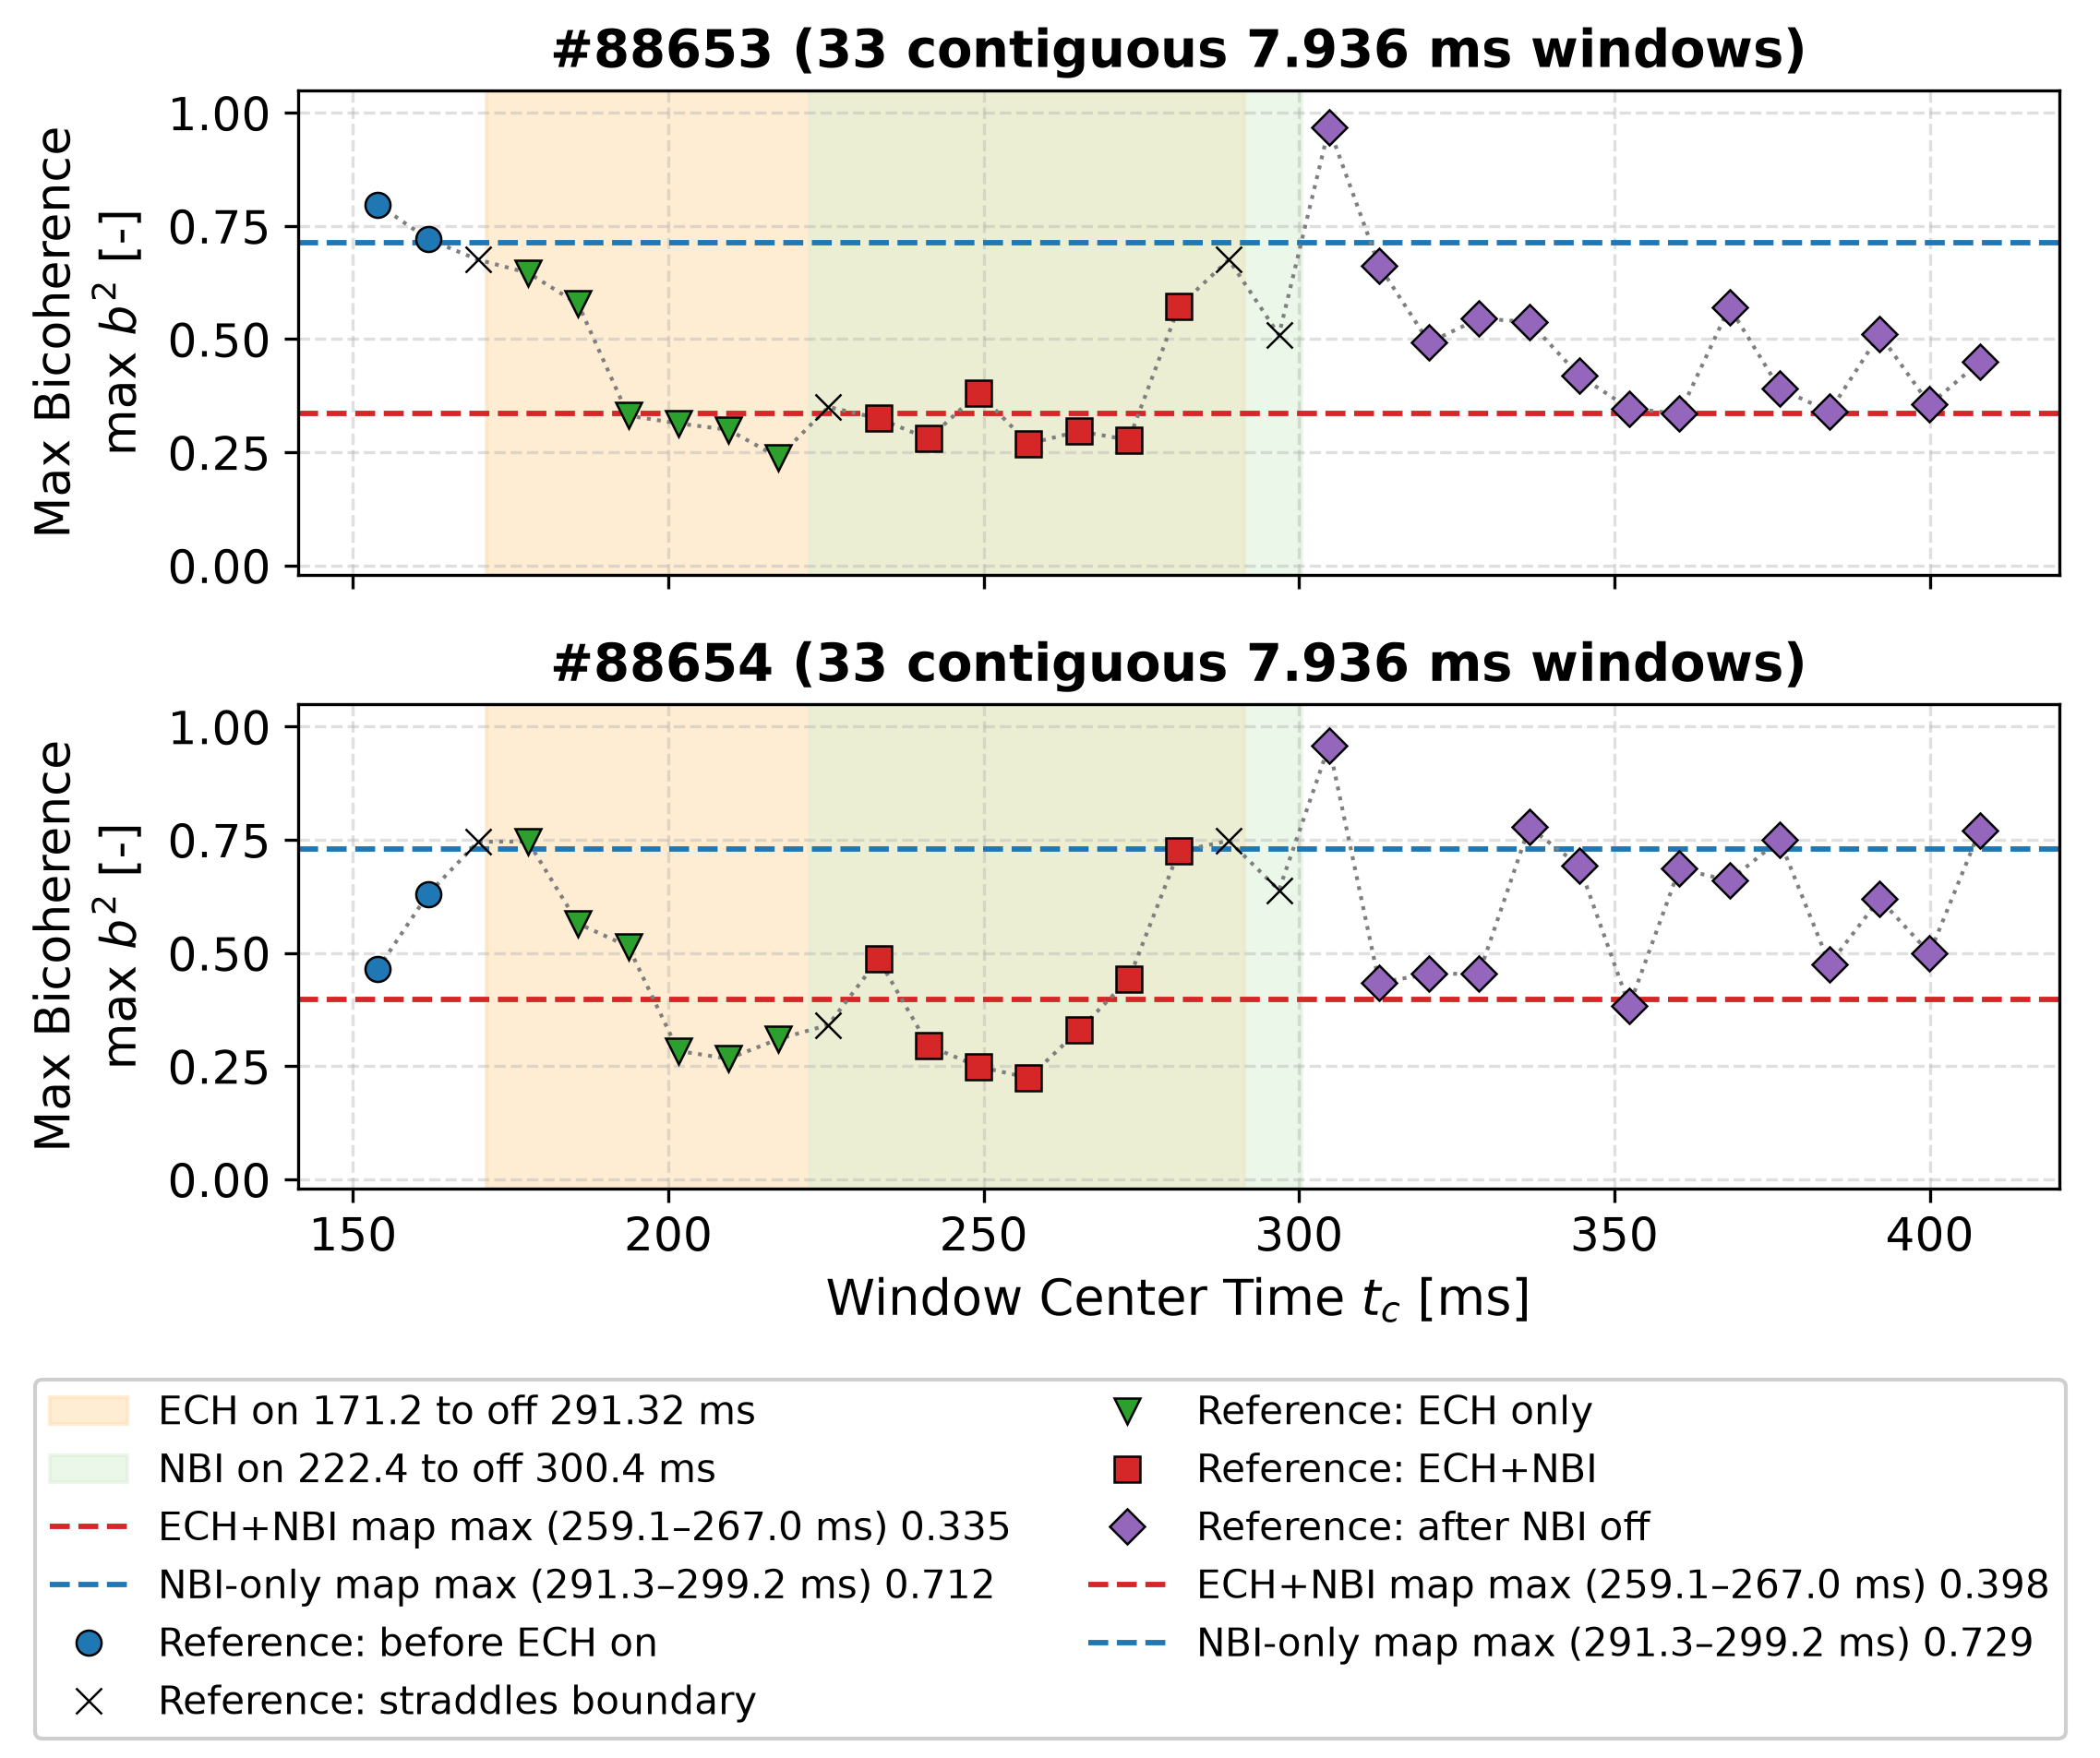
\includegraphics[width=0.75\textwidth]{Images/obj3_nonlinear_coupling/fig_control_windows_v2.png}
  \caption[Distribution of maximum squared bicoherence across reference windows]{Maximum $b^2$ ($5\text{--}100~\mathrm{kHz}$) across $33$ reference windows versus heated map maxima (dashed) for \#88653 and \#88654.}
  \label{fig:obj3_control_windows}
\end{figure}

\begin{figure}[htbp]
  \centering
  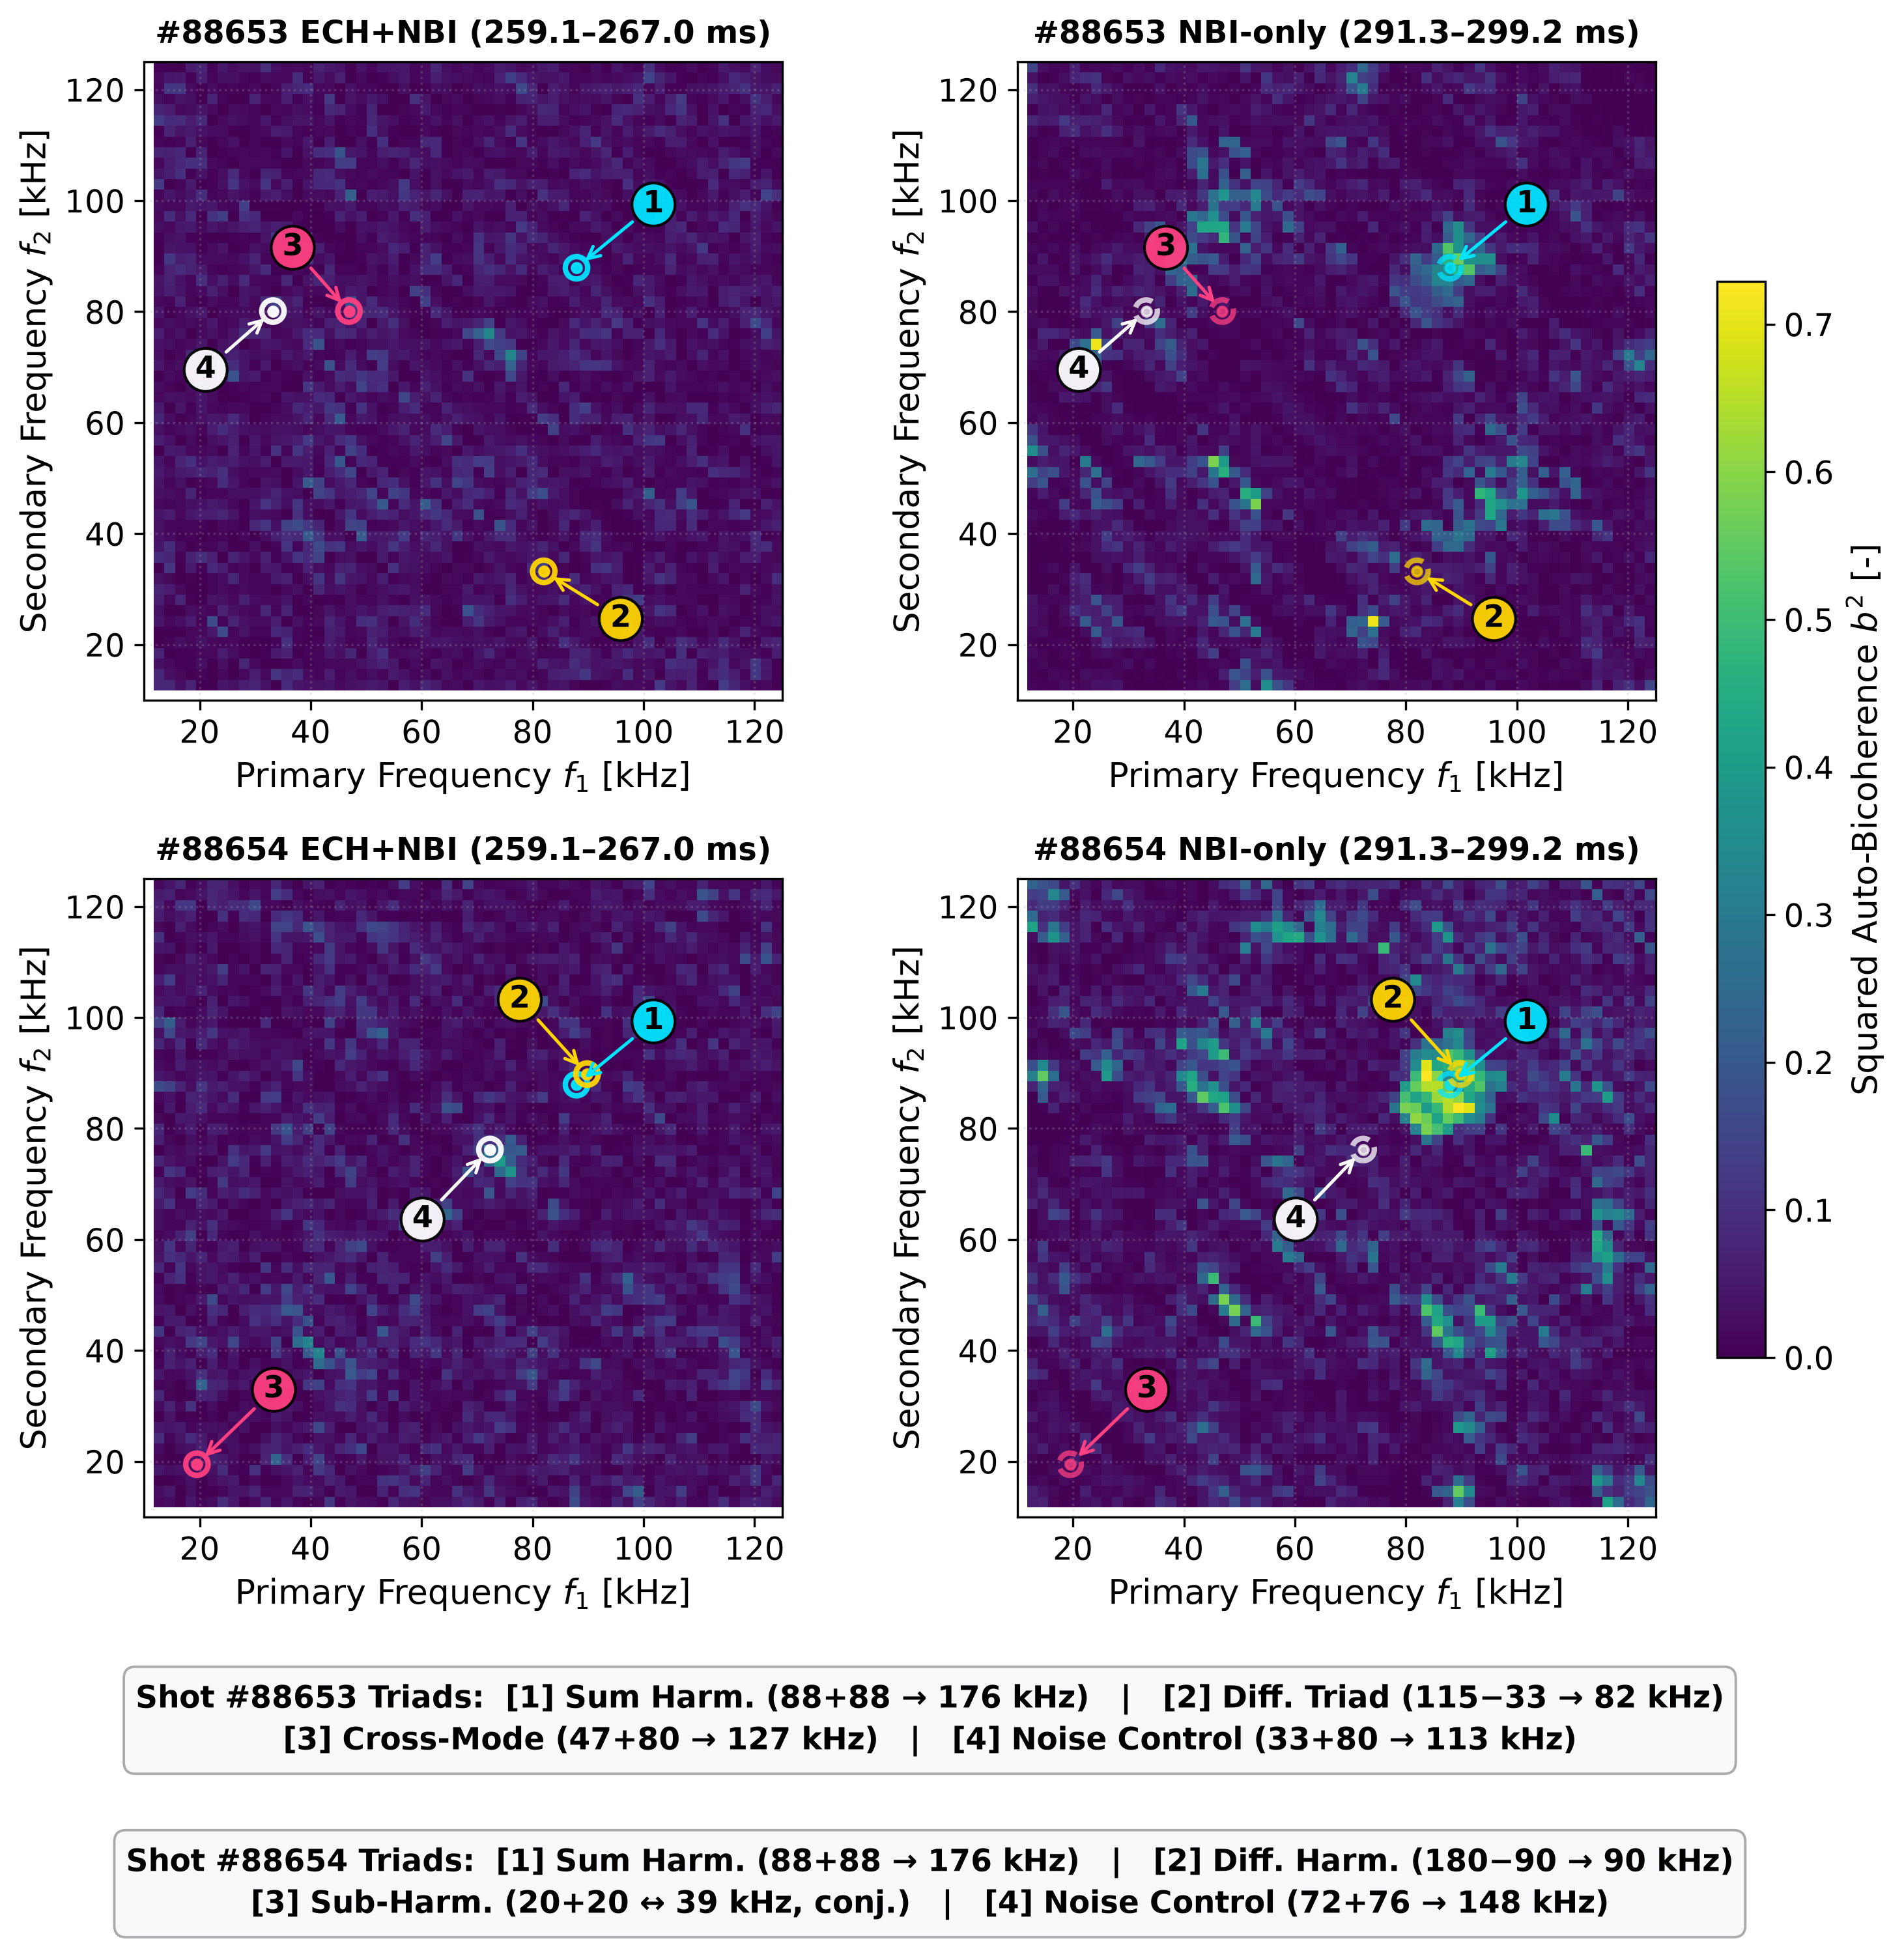
\includegraphics[width=0.88\textwidth]{Images/obj3_nonlinear_coupling/fig_bicoherence_maps_both_shots.png}
  \caption[Bicoherence maps, both shots]{Corrected MP1 $b^2(f_1, f_2)$ maps in $\mathrm{ECH}+\mathrm{NBI}$ and $\mathrm{NBI}$-only phases ($10\text{--}125~\mathrm{kHz}$) with triad markers [1]--[4].}
  \label{fig:bicoh_maps_both}
\end{figure}
Figures~\ref{fig:obj3_control_windows} and~\ref{fig:bicoh_maps_both} and Table~\ref{tab:bicoherence_maps} compared MP1 $b^2(f_1, f_2)$ in the $\mathrm{ECH}+\mathrm{NBI}$ ($259.1\text{--}267.0~\mathrm{ms}$) and $\mathrm{NBI}$-only ($291.3\text{--}299.2~\mathrm{ms}$) $7.936~\mathrm{ms}$ slices ($30$ segments) against the $33$ reference windows (with map markers [1]--[4] identifying the convergence-test primary harmonic, difference or conjugate triad, cross/sub-harmonic coupling, and noise baseline). Although $\mathrm{d}W_p/\mathrm{d}t$ regression was not performed directly, these windows evaluated nonlinear coupling inside the stored-energy regimes of Section~\ref{subsubsec:obj1_ech_off}. Over identical $7936$-sample slices, full-quadrant maxima in Figure~\ref{fig:bicoh_maps_both} matched detrended $5\text{--}100~\mathrm{kHz}$ maxima in Table~\ref{tab:bicoherence_maps} within $10^{-5}$. In $\mathrm{ECH}+\mathrm{NBI}$, map maxima ($0.335$ in \#88653; $0.398$ in \#88654) were exceeded by $23/33$ ($18/23$ non-overlapping) and $24/33$ ($19/23$) reference windows, respectively. In $\mathrm{NBI}$-only, maxima reached $0.712$ (\#88653, exceeded by $3/33$) and $0.729$ (\#88654, exceeded by $7/33$) from off-target peaks near $(23.4, 74.2)$ and $(84.0, 89.8)~\mathrm{kHz}$. Because domain maxima inflated false positives, $259.1~\mathrm{ms}$ overlapped the $261.1~\mathrm{ms}$ reference window, and reference windows mixed heating phases, raw map maxima remained \emph{inconclusive} alone.


\begin{table}[H]
\centering
\small
\caption[Bicoherence map maxima in heated and reference windows]{Bicoherence map maxima in heated and reference windows.}
\label{tab:bicoherence_maps}
\sbox0{%
\begin{tabular}{llcccc}
\toprule
Shot & Window type & Window (ms) & Map max $b^2$ (-) & Reference windows above / 33 & Reference windows above / 23 \\
\midrule
\#88653 & ECH+NBI & 259.1--267.0 & 0.335 & 23/33 & 18/23 \\
\#88653 & NBI-only & 291.3--299.2 & 0.712 & 3/33 & 3/23 \\
\#88653 & Reference windows & -- & median 0.419 [0.239, 0.967] & $N=33$ & median 0.492, $N=23$ \\
\#88654 & ECH+NBI & 259.1--267.0 & 0.398 & 24/33 & 19/23 \\
\#88654 & NBI-only & 291.3--299.2 & 0.729 & 7/33 & 6/23 \\
\#88654 & Reference windows & -- & median 0.499 [0.224, 0.958] & $N=33$ & median 0.565, $N=23$ \\
\bottomrule
\end{tabular}}
\ifdim\wd0>\textwidth\resizebox{\textwidth}{!}{\usebox0}\else\usebox0\fi
\par\smallskip{\footnotesize Strict comparison ($>$); bracketed values denote min--max range, not uncertainties. Reference set: 33 contiguous 7.936~ms windows from 150~ms (23 excluding NBI overlap; not a heating-free null).}
\end{table}


\subsubsection{Split-Sample General Search and Convergence Analysis}
\label{subsubsec:obj3_convergence}
To test whether elevated bicoherence represented genuine three-wave coupling rather than finite-sample bias, candidate peaks over $11.7\text{--}99.6~\mathrm{kHz}$ ($f_1 \le f_2$) were selected on selection segments and evaluated inside the $\mathrm{ECH}+\mathrm{NBI}$ window ($259.1\text{--}291.2~\mathrm{ms}$) across eight sub-ensemble counts $K$ ($500$ random $K$-segment subsets without replacement) on disjoint estimation blocks ($N_{\mathrm{est}}=40$ estimation segments in \#88653; $N=124$ segments in \#88654; Figure~\ref{fig:bicoh_general_search}). Extrapolating $b^2(K) = b_0 + C/K$ to $1/K \to 0$ isolated the asymptotic intercept $b_0$, and each cell was checked unpooled across all segments of the corresponding \#88654 window (Table~\ref{tab:convergence_general}).

\begin{figure}[H]
  \centering
  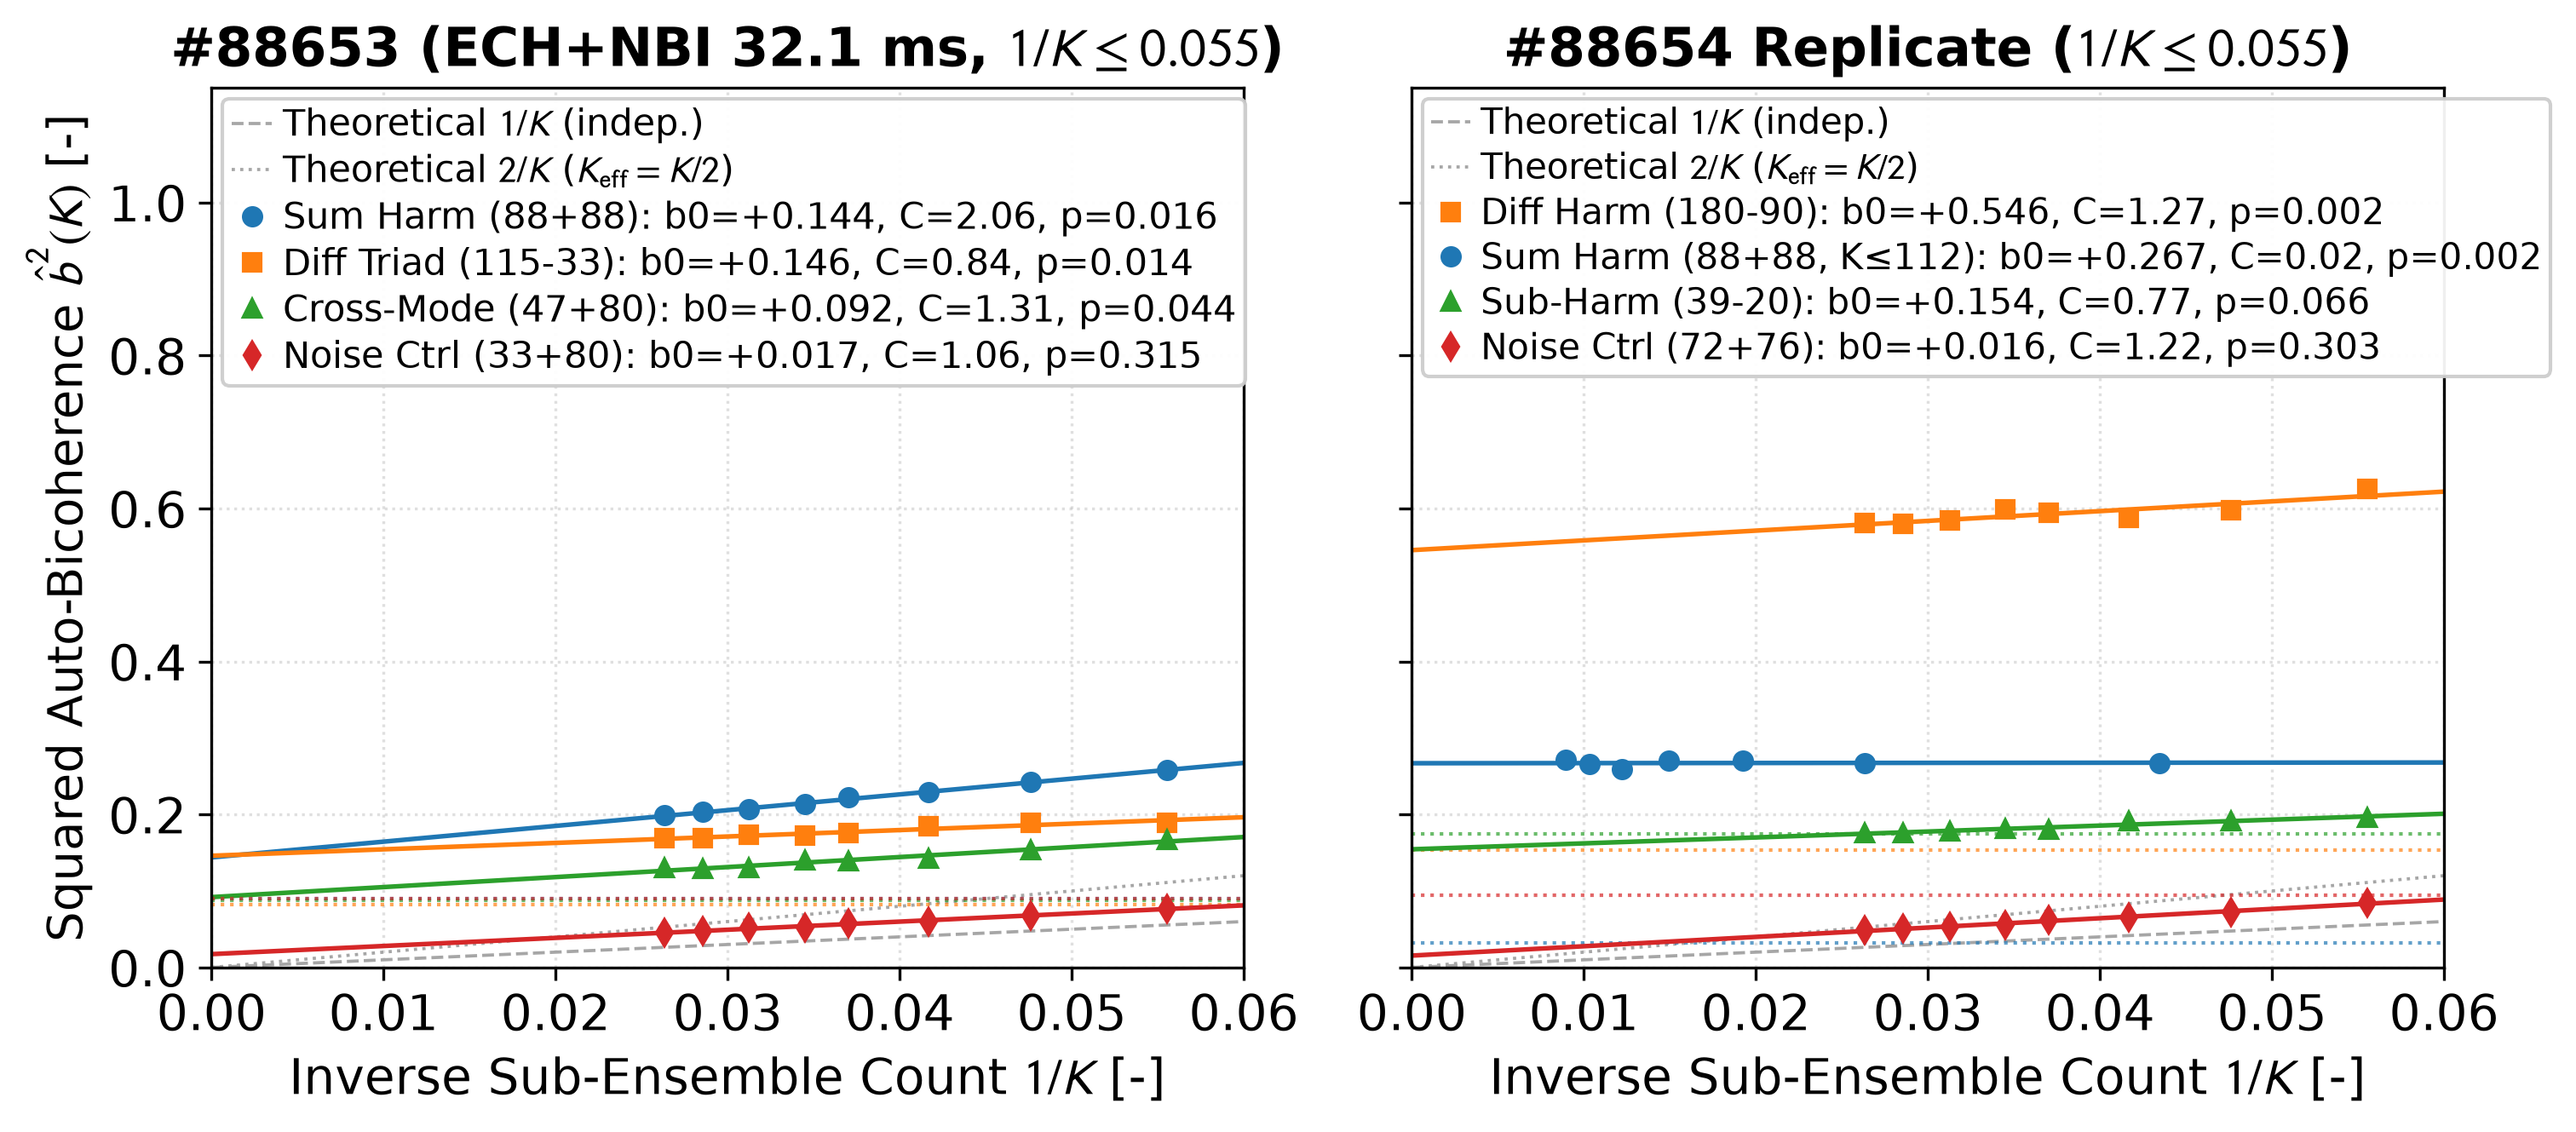
\includegraphics[width=0.90\textwidth]{Images/obj3_nonlinear_coupling/fig_convergence_cumulative_v3_general.png}
  \caption[General search: asymptotic convergence of the strongest peaks in both shots]{Asymptotic $b^2(K)$ convergence ($1/K \le 0.055$) in $\mathrm{ECH}+\mathrm{NBI}$ for shot \#88653 (left) and replicate \#88654 (right).}
  \label{fig:bicoh_general_search}
\end{figure}
\begin{table}[H]
\centering
\footnotesize
\linespread{0.91}\selectfont
\setlength{\tabcolsep}{2.95pt}
\setlength{\aboverulesep}{2pt}
\setlength{\belowrulesep}{2pt}
\renewcommand{\arraystretch}{0.92}
\caption[Asymptotic bicoherence convergence in the ECH+NBI window]{Asymptotic bicoherence convergence in the ECH+NBI window.}
\label{tab:convergence_general}
\begin{tabular}{@{}l >{\raggedright\arraybackslash}m{3.00cm} >{\centering\arraybackslash}m{3.32cm} c c c >{\raggedright\arraybackslash}m{3.68cm}@{}}
\toprule
Discharge & \shortstack[l]{Triad\\Type} & \shortstack{$f_1, f_2 \to f_3$\\(kHz)} & \shortstack{Intercept\\$b_0$ (-)} & \shortstack{Slope\\$C$ (-)} & \shortstack{Surrogate\\$p_{\rm surr}$ (-)} & \shortstack[l]{Validation Status\\($p < 0.05$)} \\
\midrule
\#88653 & Primary Sum Harmonic & $87.9 + 87.9 \to 175.8$ & $+0.144$ & $2.06$ & $0.016$ & Validated ($2/K$ overlap scaling) \\
\#88653 & Difference Triad & $115.2 - 33.2 \to 82.0$ & $+0.146$ & $0.84$ & $0.014$ & Validated (Inter-mode coupling) \\
\#88653 & Cross-Mode Interaction & $46.9 + 80.1 \to 127.0$ & $+0.092$ & $1.31$ & $0.044$ & Validated (Secondary-\newline to-primary flank) \\
\#88653 & Noise Contrast Baseline & $33.2 + 80.1 \to 113.3$ & $+0.017$ & $1.06$ & $0.315$ & Negative Control ($1/K \to 0$) \\
\midrule
\#88654 & Primary Harmonic\newline (Diff./Conj.) & $(89.8, 89.8) \leftrightarrow 179.7$\newline $(179.7\!-\!89.8\!\to\!89.8)$ & $+0.546$ & $1.27$ & $0.002$ & Validated (Adjacent-bin\newline conjugate replicate) \\
\#88654 & Primary Sum Harmonic & $87.9 + 87.9 \to 175.8$ & $+0.267$ & $0.02$ & $0.002$ & Validated (Cross-shot\newline harmonic replicate) \\
\#88654 & Sub-Harmonic Triad & $39.1 - 19.5 \to 19.5$ & $+0.154$ & $0.77$ & $0.066$ & Candidate (Marginal significance) \\
\#88654 & Noise Contrast Baseline & $72.3 + 76.2 \to 148.4$ & $+0.016$ & $1.22$ & $0.303$ & Negative Control ($1/K \to 0$) \\
\bottomrule
\end{tabular}
\par\vspace{2pt}\noindent\parbox{\textwidth}{\footnotesize ECH+NBI window ($259.1\text{--}291.2~\mathrm{ms}$), asymptotic regime $1/K \le 0.055$ ($K \ge 18$); \#88653 ($N_{\mathrm{est}}=40$), \#88654 ($N=124$). Mean of 500 random sub-ensembles without replacement ($95\,\%$ bounds $[q_{2.5}, q_{97.5}]$ reflect finite-$K$ sub-ensemble dispersion, whereas $p_{\rm surr}$ tests mean $b_0$ vs.\ 500 phase-randomized surrogates). In \#88654, marker~[2] at $(f_1, f_2) = (89.8, 89.8)~\mathrm{kHz}$ (adjacent to $(87.9, 87.9)~\mathrm{kHz}$ within the scanned $f_1, f_2 \in [11.7, 99.6]~\mathrm{kHz}$ plane) couples the fundamental $89.8~\mathrm{kHz}$ mode with its second harmonic at $f_1 + f_2 = 179.7~\mathrm{kHz}$---equivalent by Hermitian conjugate symmetry to $179.7 - 89.8 \to 89.8~\mathrm{kHz}$---marking an adjacent-bin conjugate realization of the same primary self-harmonic steepening over $N=124$ rather than an independent triad. The brief $8.7~\mathrm{ms}$ NBI-only interval ($291.3\text{--}300.0~\mathrm{ms}$, $N_{\mathrm{seg}}=32$) yielded only $2$ estimation units ($<6$ required) and was \emph{untestable} in both \#88653 and \#88654.}
\end{table}

In Figure~\ref{fig:bicoh_general_search} (showing subset means against theoretical $1/K$ and $2/K$ lines, dotted horizontal $95~\%$ surrogate nulls, and legend parameters $(b_0, C, p_{\mathrm{surr}})$) and Table~\ref{tab:convergence_general}, restricting fits to $1/K \le 0.055$ ($K \ge 18$, including $K \le 112$ over $N=124$ for the \#88654 sum harmonic) eliminated small-ensemble curvature bias and yielded tight linear regressions ($R^2 \ge 0.96\text{--}0.99$). Three candidate triads in \#88653 cleared the $500$-surrogate null ($p_{\mathrm{surr}} < 0.05$). First, primary-mode self-harmonic steepening (marker~[1], $(87.9, 87.9) ~\mathrm{kHz}\to 175.8~\mathrm{kHz}$) reached $b_0 = +0.144$ ($p_{\mathrm{surr}} = 0.0160$, testing the mean intercept against $500$ phase-randomized surrogates) along the $2/K$ overlap slope ($C = +2.06$), with finite-$K$ dispersion $[q_{2.5}, q_{97.5}] = [-0.029, +0.320]$. Second, a difference triad (marker~[2], $(115.2, -33.2)~\mathrm{kHz}\to 82.0~\mathrm{kHz}$) converged to $b_0 = +0.146$ ($p_{\mathrm{surr}} = 0.0140$). Third, a sum triad coupling the secondary mode to the primary flank (marker~[3], $(46.9, 80.1)~\mathrm{kHz}\to 127.0~\mathrm{kHz}$) converged to $b_0 = +0.092$ ($p_{\mathrm{surr}} = 0.0439$). Conversely, the off-diagonal noise baseline (marker~[4], $(33.2, 80.1)\to 113.3~\mathrm{kHz}$) followed the theoretical $1/K$ slope ($C = +1.06$) directly to zero ($b_0 = +0.017 \approx 0.000$, $p_{\mathrm{surr}} = 0.3154$).

In replicate \#88654 ($N = 124$ segments), primary harmonic steepening remained validated in both the conjugate difference ($(179.7, -89.8)~\mathrm{kHz}\to 89.8~\mathrm{kHz}$, $b_0 = +0.546$, $p_{\mathrm{surr}} = 0.0020$) and sum channels ($(87.9, 87.9)~\mathrm{kHz}\to 175.8~\mathrm{kHz}$, $b_0 = +0.267$, $p_{\mathrm{surr}} = 0.0020$). Specifically, in \#88654 (scanned plane $f_1, f_2 \in [11.7, 99.6]~\mathrm{kHz}$), marker~[2] at $(89.8, 89.8)~\mathrm{kHz}$ (adjacent to $(87.9, 87.9)~\mathrm{kHz}$) coupled the $89.8~\mathrm{kHz}$ fundamental with $f_1+f_2=179.7~\mathrm{kHz}$---conjugate-equivalent to $179.7~\mathrm{kHz} -89.8 ~\mathrm{kHz}\to 89.8~\mathrm{kHz}$ in Table~\ref{tab:convergence_general}---marking the same self-harmonic steepening, while marker~[3] at $(19.5, 19.5)~\mathrm{kHz}$ corresponded via conjugate symmetry to the marginal sub-harmonic triad $39.1~\mathrm{kHz} -19.5~\mathrm{kHz}\to 19.5~\mathrm{kHz}$ ($b_0=+0.154$, $p_{\mathrm{surr}}=0.066$). Meanwhile, its noise baseline (marker~[4], $72.3 ~\mathrm{kHz} + 76.2 ~\mathrm{kHz}\to 148.4~\mathrm{kHz}$ in Table~\ref{tab:convergence_general}) decayed along $1/K$ directly to zero ($b_0 = +0.016$, $p_{\mathrm{surr}} = 0.3034$). In contrast, the brief $8.7~\mathrm{ms}$ $\mathrm{NBI}$-only phase ($291.3\text{--}300.0~\mathrm{ms}$, $N_{\mathrm{seg}} = 32$) yielded only $2$ disjoint estimation blocks, below the $6$-block minimum required for unbiased split-sample regression, and was therefore classified as \emph{untestable} in both \#88653 and \#88654.

Whereas preliminary single-window evaluations using the uncorrected \texttt{jpack} estimator appeared inconclusive due to the one-bin \texttt{np.roll} offset and finite-sample bias, rectifying the index lookup and extrapolating $b^2(K)$ over $1/K \le 0.055$ cleanly isolated this quadratic phase locking. Consistent with bispectral theory~\cite{KimPowers1979} and helical/tokamak studies~\cite{Kin2025,Miyashita2025,Hou2019}, positive asymptotic intercepts ($b_0 > 0$) versus $1/K \to 0$ baseline decay confirmed genuine quadratic phase locking among the primary mode, its second harmonic, and lower-frequency fluctuations.

\subsection[Integrated Physical Discussion and Quantitative Literature Contrast]{Integrated Physical Discussion and Quantitative\\ Literature Contrast}
\label{subsec:integrated_discussion}
A first-principles order-of-magnitude Alfv\'enic scaling analysis supports the physical assignment of both coherent frequency bands in Heliotron~J. For standard parameters ($B_0 = 1.25~\mathrm{T}$, $n_e \approx 0.6\text{--}1.0 \times 10^{19}~\mathrm{m^{-3}}$, $R_0 = 1.2~\mathrm{m}$, $\iota/2\pi \approx 0.56$), Eq.~(\ref{eqn:alfven}) yields $v_A \approx 6.1\text{--}7.9 \times 10^6~\mathrm{m/s}$ ($f_{\mathrm{TAE}} = (\iota/2\pi)v_A/(4\pi R_0) \approx 226\text{--}292~\mathrm{kHz}$) for pure deuterium ($m_i = 2 m_p$), and $v_A \approx 6.1\text{--}11.2 \times 10^6~\mathrm{m/s}$ ($f_{\mathrm{TAE}} \approx 226\text{--}412~\mathrm{kHz}$) across mixed hydrogen--deuterium NBI plasmas ($m_{\mathrm{eff}} \approx 1.0\text{--}2.0\,m_p$). Both observed bands ($40\text{--}50~\mathrm{kHz}$ and $86\text{--}90~\mathrm{kHz}$) therefore lie well below the TAE continuum gap ($> 220~\mathrm{kHz}$), ruling out a standard gap TAE and pointing instead to lower-frequency BAE or resonant EPM branches. Evaluating the BAE/GAM acoustic baseline in Eq.~(\ref{eqn:f_bae_baseline}),
\begin{equation}
\label{eqn:f_bae_baseline}
f_{\mathrm{BAE}} \approx \frac{1}{2\pi R_0}\sqrt{\frac{2 k_B T_i}{m_i}\left(\frac{7}{4} + \frac{T_e}{T_i}\right)},
\end{equation}
where $R_0$ is the major radius ($\mathrm{m}$), $k_B$ is the Boltzmann constant ($\mathrm{J/K}$), $m_i$ is the effective ion mass ($\mathrm{kg}$), and $T_e$ and $T_i$ are the core electron and ion temperatures ($\mathrm{K}$), for typical Heliotron~J core conditions under $\mathrm{ECH}+\mathrm{NBI}$ ($T_e \approx 0.3\text{--}0.8~\mathrm{keV}$, $T_i \approx 0.15\text{--}0.3~\mathrm{keV}$) yields an ion-acoustic speed $c_s = \sqrt{k_B T_e / m_i} \approx 1.2\text{--}2.0 \times 10^5~\mathrm{m/s}$ (pure $\mathrm{D}_2$) and $f_{\mathrm{BAE}} \approx 31\text{--}47~\mathrm{kHz}$ ($\approx 31\text{--}55~\mathrm{kHz}$ across $m_{\mathrm{eff}} \approx 1.5\text{--}2.0\,m_p$) in quantitative agreement with the observed $40\text{--}50~\mathrm{kHz}$ secondary mode (consistent with the Eq.~(\ref{eqn:gam}) $\sqrt{T_e}$ proxy because $\frac{7}{4}T_i + T_e$ is electron-dominated at $T_e > T_i$), while finite-$k_\parallel$ Alfv\'en--acoustic coupling ($\sqrt{v_A^2 k_\parallel^2 + \omega_{\mathrm{BAE}}^2}/(2\pi)$ for small effective $|k_\parallel R_0| \sim 0.04\text{--}0.12$) spans $80\text{--}100~\mathrm{kHz}$; because unshifted vacuum $|m(\iota/2\pi) - n| > 1$ for $m = +3$ and $n \equiv -1 \pmod 4$ at $\iota/2\pi \approx 0.56$, placing the $86\text{--}90~\mathrm{kHz}$ primary branch in this range points either to helical $M = 4$ sideband coupling or fast-ion resonant EPM drive (Eq.~(\ref{eqn:condition})). Contrasting these findings with prior Heliotron~J investigations highlights strong continuity alongside configuration-specific distinctions. Yamamoto \emph{et~al.}~\cite{Yamamoto_2020}, Varela \emph{et~al.}~\cite{Varela2023}, and Zhong \emph{et~al.}~\cite{Zhong2024} report NBI-driven core EPMs across $60\text{--}120~\mathrm{kHz}$ modulated by ECH/ECCD electron heating, matching the $86\text{--}90~\mathrm{kHz}$ ($m = +3$, $n \equiv -1 \pmod 4$) primary branch and the ECH-off sensitivity of the $40\text{--}50~\mathrm{kHz}$ secondary branch. Likewise, 3D gyrofluid simulations by Varela \emph{et~al.}~\cite{Varela2015} confirm that low-$n$ EPM/BAE drive tracks fast-ion pressure gradients inside the core-to-mid zone ($\rho \approx 0.29\text{--}0.47$). By contrast, Zang \emph{et~al.}~\cite{zang2019observation} observe an outer-gradient BAE/global Alfv\'en eigenmode (GAE)-band instability at $\rho = 0.86\text{--}0.91$ with $m \sim 6\text{--}8$. The modes isolated here peak deeper in the core ($\rho_{\mathrm{centroid}} \approx 0.38$, $m = +3$ and coexisting $m_1 = +1$ global / $m_2 = +12$ components). Furthermore, the outward ECE wavepacket group velocity ($v_{\mathrm{g},r} \approx +22$ to $+36~\mathrm{km/s}$) extends prior Heliotron~J fluctuation radiometry~\cite{luo2020measurement} to resolved core energy propagation. The asymptotic bicoherence intercepts ($b_0 = +0.092$ to $+0.546$) also align quantitatively with nonlinear mode--turbulence and Alfv\'enic couplings in Heliotron~J~\cite{Kin2025,Miyashita2025} and the HL-2A tokamak~\cite{Hou2019}. Table~\ref{tab:literature_contrast} synthesizes this quantitative benchmark against prior helical and tokamak studies.

\begin{table}[H]
  \centering
  \caption[Quantitative comparison between the present Heliotron~J study and prior literature]{Quantitative comparison between the present Heliotron~J study and prior literature.}
  \label{tab:literature_contrast}
  \footnotesize
  \setlength{\tabcolsep}{4pt}
  \renewcommand{\arraystretch}{1.18}
  \begin{tabular}{>{\raggedright\arraybackslash}p{0.19\textwidth}>{\raggedright\arraybackslash}p{0.20\textwidth}>{\raggedright\arraybackslash}p{0.25\textwidth}>{\raggedright\arraybackslash}p{0.28\textwidth}}
    \toprule
    \textbf{Study (Device)} & \textbf{Regime \& Diagnostics} & \textbf{Observed Mode \& Scaling} & \textbf{Key Benchmark Contrast} \\
    \midrule
    Yamamoto \emph{et~al.}~\cite{Yamamoto_2020} (Heliotron~J) & NBI + ECH/ECCD; Mirnov arrays & Core EPMs ($60\text{--}120~\mathrm{kHz}$); ECH/ECCD shift & Matches $86\text{--}90~\mathrm{kHz}$ ($m=+3$) band; extended here to 18-coil $\times$ 16-ECE mapping \\
    Zhong \emph{et~al.}~\cite{Zhong2024} \& Varela \emph{et~al.}~\cite{Varela2023} (Heliotron~J) & NBI + modulated ECH; Mirnov \& $W_p$ & Core EPM/BAE ($60\text{--}120~\mathrm{kHz}$); ECH-driven $\Delta f$ & Mirrors $-9.69~\mathrm{kHz}$ ECH-off step ($p_{\mathrm{surr}} = 0.004$); shown non-reducible to $n_e$ (explaining $\le 26.2~\%$ of $\Delta f$) \\
    Zang \emph{et~al.}~\cite{zang2019observation} (Heliotron~J) & NBI; Mirnov \& radial arrays & Outer BAE/GAE ($\rho = 0.86\text{--}0.91$, $m \sim 6\text{--}8$) & Modes here peak deeper ($\rho \approx 0.29\text{--}0.47$, centroid $0.38$) with $m=+3$ and $(+1, +12)$ \\
    Varela \emph{et~al.}~\cite{Varela2015,Varela2024} (Heliotron~J, TJ-II) & FAR3d 3D gyrofluid modeling & Low-$n$ core-to-mid EPM/BAE ($\nabla p_f$ drive) & Equilibrium drive zone matches measured $\rho \approx 0.29\text{--}0.47$ and $n \equiv -1 \pmod 4$ \\
    Luo \emph{et~al.}~\cite{luo2020measurement} \& Weir~\cite{Weir2019} (Heliotron~J) & 16-channel / correlation ECE ($57.5\text{--}72.5~\mathrm{GHz}$) & Internal $T_e$ fluctuation radiometry & Extended to inward carrier tilt ($\Delta\tau = -0.39$ to $-0.51~\mu\mathrm{s}$) vs. outward $v_{\mathrm{g},r} \approx +22$ to $+36~\mathrm{km/s}$ \\
    Kin \emph{et~al.}~\cite{Kin2025} \& Hou \emph{et~al.}~\cite{Hou2019} (Heliotron~J, HL-2A) & Higher-order auto-bicoherence $b^2$ & Nonlinear mode--turbulence / Alfv\'en coupling & Isolated via $1/K \to 0$ intercept ($b_0 = +0.092$ to $+0.546$, $p_{\mathrm{surr}} \le 0.0439$) vs. $O(1/K)$ null \\
    \textbf{Present work} (Heliotron~J, \#88653/4) & 18 Mirnov + 16 ECE + $W_p, I_p, n_e$; Python/NUDFT & Primary $86\text{--}90~\mathrm{kHz}$ ($m=+3$); secondary $40\text{--}50~\mathrm{kHz}$ & Rectified $1.953~\mathrm{kHz}$ \texttt{jpack} shift; Bartlett $N_{\mathrm{eff}}$, FDR-BH, and $500$-surrogate bounds \\
    \bottomrule
  \end{tabular}
\end{table}

From an experimental-design standpoint, evaluating the matched control-versus-perturbation pair (\#88653 primary and \#88654 unpooled replicate) avoids artificial sample pooling while retaining substantial within-discharge statistical power. Rather than treating $N = 2$ as an underpowered macro-sample, inference operates over $262\,144$ samples per $1~\mathrm{MHz}$ diagnostic trace, $18 \times 16 = 288$ cross-diagnostic coil--radiometer spatial pairs, $33$ contiguous empirical reference windows, and $80\text{--}124$ overlapping spectral segments per heating phase, all calibrated via Bartlett autocorrelation $N_{\mathrm{eff}}$, FDR-BH multiplicity control, and $500$ phase-randomized surrogates. Concurrently, negative partial correlations and non-significant dispersion $p_{\mathrm{adj}}$ define exact empirical sensitivity limits without overclaiming causality.

Synthesizing Objectives~1--3 establishes a unified, quantitatively bounded view of multi-diagnostic MHD behavior across heated Heliotron~J discharges. Objective~1 confirms that NBI fast ions destabilize core helical modes ($m = +3$ and $m_1 = +1$, $n \equiv -1 \pmod 4$) whose wavepackets propagate outward ($v_{\mathrm{g},r} \approx +22~\mathrm{km/s}$ to $+36~\mathrm{km/s}$). Across ECH switch-off, these modes persist with a $-9.69~\mathrm{kHz}$ secondary-centroid shift ($-9.86~\mathrm{kHz}$ in \#88654) and a $-54.3~\mathrm{kW}$ to $-81.1~\mathrm{kW}$ $\mathrm{d}W_p/\mathrm{d}t$ step ($-54.3~\mathrm{kW}$ to $-60.9~\mathrm{kW}$ in \#88653; $-68.3~\mathrm{kW}$ to $-81.1~\mathrm{kW}$ in \#88654) driven primarily by ECH power removal. Objective~2 evaluates lagged envelope correlations, showing that shared heating ramps ($N_{\mathrm{eff}} \approx 15.8\text{--}34.1$) yield near-zero step-controlled partial correlations. It also verifies a $30~\mathrm{Hz}$ LPF ECE relative thermal proxy (\texttt{ECE12FAST} core and \texttt{ECE9FAST} chord-integrated) and identifies positive, physically consistent (though statistically non-significant, $p_{\mathrm{adj}} = 0.099\text{--}0.162$) tendencies toward candidate $\sqrt{T_e}$ and $\sqrt{v_A^2 + c_s^2}$ BAE scalings. Objective~3 demonstrates that combined $\mathrm{ECH}+\mathrm{NBI}$ heating exhibits validated self-harmonic steepening ($87.9 + 87.9~\mathrm{kHz} \to 175.8~\mathrm{kHz}$, $b_0 > 0$, $p_{\mathrm{surr}} < 0.05$) and inter-mode phase locking against $500$ surrogates, separating true coupling from $O(1/K) \to 0$ noise.

These validated tools and findings provide concrete institutional value across both partner laboratories. At IAE, Kyoto University, the rectified \texttt{jpack} auto-bicoherence routine (\texttt{abicoh2\_\allowbreak corrected.py}, fixing the $1.953~\mathrm{kHz}$ one-bin shift) and automated \texttt{.json} and spectrogram mode-cataloging pipeline integrate directly into daily Heliotron~J campaign analysis to replace manual shot screening. Simultaneously, at PlasmaTEC, ITCR, these methods transfer directly to possible Mirnov and Langmuir probe diagnostics on the Stellarator of Costa Rica~1 (SCR-1) and spherical torus experiments. In particular, the NUDFT array decomposition, Bartlett $N_{\mathrm{eff}}$ auditing, and surrogate-calibrated $1/K$ bicoherence workflow isolate true couplings from finite-sample variance.

\clearpage
\newpage
\section{Conclusions and Recommendations}
\label{sec:conclusions}

\subsection{Conclusions}
\label{subsec:conclusions}

Through an automated open-source Python pipeline applied to Heliotron~J shots \#88653 and unpooled replicate \#88654, the three specific objectives and general objective achieved distinct, rigorously bounded fulfillment outcomes. \textbf{Specific Objective~1} was \emph{fulfilled} within diagnostic array limits: dual-criterion gating ($3\sigma$ dominance and $\gamma^2 > 0.7$) isolated the $86\text{--}90~\mathrm{kHz}$ ($m=+3$) primary and $40\text{--}50~\mathrm{kHz}$ ($m_1=+1, m_2=+12$) secondary modes ($n \equiv -1 \pmod 4$) inside $\rho \approx 0.29\text{--}0.47$, noting that toroidal mode numbers were resolved modulo~$4$ and the steep $m_2 = +12$ branch neared the 14-coil Nyquist limit. Phase-lag tracking further separated inward carrier delays from outward wavepacket propagation and established the $-9.69~\mathrm{kHz}$ ECH-off secondary centroid drop ($p_{\mathrm{surr}} = 0.004$), whereas discrete secondary peak shifts ($p_{\mathrm{surr}} = 0.124$), primary-band ECH-off frequency steps ($p_{\mathrm{surr}} = 0.194\text{--}0.240$), and density-scaling attribution (explaining $17.8\text{--}26.2~\%$ of the frequency drop) remained \emph{inconclusive}. \textbf{Specific Objective~2} was \emph{methodologically fulfilled} yet \emph{partially fulfilled / statistically inconclusive} in causal physics: ECH-step partial correlations collapsed to $r_{\mathrm{partial}} \approx 0.002\text{--}0.076$, precluding causal proof from lagged macroscopic correlations ($N_{\mathrm{eff}} \approx 15.8\text{--}34.1$), and while the $30~\mathrm{Hz}$ low-pass ECE proxy revealed positive candidate BAE tendencies ($\sqrt{T_e}$ and $\sqrt{v_A^2+c_s^2}$, $p_{\mathrm{adj}} = 0.099\text{--}0.162$), no dispersion model cleared $|r| > 0.70$ at $p_{\mathrm{adj}} < 0.05$. \textbf{Specific Objective~3} was \emph{fulfilled} in the $\mathrm{ECH}+\mathrm{NBI}$ regime via rectified \texttt{jpack} auto-bicoherence and $1/K \to 0$ surrogate convergence ($p_{\mathrm{surr}} \le 0.0439$ for primary harmonic steepening and inter-mode locking), \emph{not supported} for unadjusted single-window map maxima or primary--secondary sum coupling in stationary \#88653, and \emph{untestable} in the brief $8.7~\mathrm{ms}$ $\mathrm{NBI}$-only interval of both \#88653 and \#88654 ($2$ blocks). Finally, the \textbf{General Objective} was \emph{fulfilled} for reproducible multi-diagnostic mode characterization under explicit statistical bounds on excitation and energy impact (where $\Delta(\mathrm{d}W_p/\mathrm{d}t) \approx -54.3$ to $-81.1~\mathrm{kW}$ primarily reflected external ECH power termination).

Collectively, these validated algorithms and bounded physical results delivered concrete scientific and methodological value to both partner institutions. For the Heliotron~J group at IAE, Kyoto University, the project delivered an index-corrected \texttt{jpack} bispectral estimator alongside a reusable multi-diagnostic mode-cataloging pipeline for routine experimental campaigns. Simultaneously, for PlasmaLabTEC at ITCR, this work established transferable capabilities in non-uniform spatial-harmonic decomposition, autocorrelation-adjusted correlation auditing, and surrogate-calibrated higher-order spectral analysis applicable to stellarator and spherical-torus confinement studies.

\subsection{Recommendations}
\label{subsec:recommendations}

To overcome the temporal and statistical constraints of the present discharge pair, future campaigns should analyze a broader multi-shot dataset. Varying ECH switch-off timings (such as \#88652 and \#83848), modulated ECH pulses, and co- versus counter-NBI heating will strengthen statistical power. Diverse heating schedules and beam directions will decouple collinear profile ramps, test fast-ion drive asymmetries, and extend $\mathrm{NBI}$-only plateaus well past $9~\mathrm{ms}$ so split-sample bicoherence convergence becomes testable across both heating phases.

From a diagnostic and equilibrium-modeling standpoint, future work should add absolute power calibrations ($\mathrm{kW}$) for \texttt{ECHRG500} and \texttt{NBIS9}/\texttt{NBIS10} to evaluate mode excitation thresholds. Integrating Thomson scattering or calibrated ECE electron temperature profiles $T_e(\rho)$, charge-exchange recombination spectroscopy (CXRS) ion temperature and rotation measurements, and 3D Variational Moments Equilibrium Code (VMEC) reconstructions of $\iota(\rho)/2\pi$ is strongly recommended. Combining calibrated profiles with the core fluctuation zone established here will enable direct testing of rational-surface alignment ($\iota/2\pi = n/m$) and quantitative Alfv\'en continuum gap calculations.

Finally, the modular pipeline should incorporate boundary and scrape-off-layer diagnostics, particularly divertor Langmuir probe arrays and fast optical monitors, into its cross-bicoherence and envelope-correlation modules. Testing cross-bicoherence among internal ECE modes, edge Mirnov coils, and divertor ion-saturation currents will directly probe whether core three-wave couplings and outward-propagating wavepackets modulate edge turbulence and cross-field particle transport.

\clearpage
\phantomsection
\addcontentsline{toc}{section}{References}
{\setlength{\parskip}{2pt}%
\bibliographystyle{IEEEtran}
\bibliography{ref}}


\clearpage
\phantomsection
\section*{Glossary}
\addcontentsline{toc}{section}{Glossary}

\begin{description}
\raggedright
\sloppy
\setlength{\itemsep}{0.2pt}
\setlength{\parsep}{0pt}
\setlength{\parskip}{0pt}
\item[Alfv\'{e}n Eigenmode (AE)] Discrete electromagnetic oscillation excited within shear-Alfv\'{e}n continuum spectral gaps created by periodic toroidal or helical variations in the confining magnetic field strength.

\item[Analytic Signal] Complex-valued time-series representation $z(t) = x(t) + \mathrm{i}\,\mathcal{H}[x(t)]$ formed from a real fluctuation signal $x(t)$ and its Hilbert transform $\mathcal{H}[x(t)]$, from which the instantaneous amplitude envelope $A(t)$ ($\mathrm{V}$) and unwrapped phase $\phi(t)$ ($\mathrm{rad}$) are extracted.

\item[Auto-bicoherence ($b^2$)] Dimensionless normalized magnitude-squared bispectrum bounded on $[0, 1]$ that quantifies the fraction of spectral power at a coupled frequency $f_3 = f_1 \pm f_2$ ($\mathrm{Hz}$) attributable to quadratic phase locking rather than independent random fluctuations.

\item[Bessel Filter] Analog or digital linear filter designed for maximally flat group delay in the passband, preserving pulse waveforms and instantaneous phase trajectories without ringing distortion across the $40\text{--}80$ and $80\text{--}120~\mathrm{kHz}$ mode bands.

\item[Beta-induced Alfv\'{e}n Eigenmode (BAE)] Low-frequency compressional shear-Alfv\'{e}n mode located below the geodesic acoustic mode (GAM) continuum gap whose frequency scales with the plasma ion-acoustic velocity ($\propto \sqrt{\tfrac{7}{4}T_i + T_e}$, with $T_e, T_i$ in $\mathrm{K}$ or $\mathrm{keV}$) and finite thermal pressure $\beta$.

\item[Bispectrum ($B$)] Third-order spectral moment $B(f_1, f_2) = \langle X(f_1) X(f_2) X^*(f_1 \pm f_2) \rangle$ ($\mathrm{V^3/Hz^3}$) probing coherent three-wave quadratic phase coupling across resonant sum or difference frequency triads $f_3 = f_1 \pm f_2$ ($\mathrm{Hz}$).

\item[Circular Concentration Coefficient ($r_{\mathrm{circ}}$)] Directional statistics metric bounded on $[0, 1]$ measuring angular clustering of spatial phase residuals across a magnetic probe array for candidate poloidal mode number $m$, where $r_{\mathrm{circ}} = 1$ indicates zero phase dispersion.

\item[Continuous Wavelet Transform (CWT)] Multiresolution time--frequency decomposition convolving a fluctuation signal against dilated copies of an analyzing wavelet (complex Morlet $\psi(t)$ in this thesis) to resolve rapid frequency chirps without fixed-window resolution trade-offs.

\item[Continuum Gap] Spectral frequency window in the continuous shear-Alfv\'{e}n spectrum opened by periodic toroidal ($R_0$) or helical ($L=1, M=4$) magnetic field variations, allowing discrete eigenmodes (such as AEs, BAEs, and TAEs) to persist with reduced continuum damping.

\item[Diamagnetic Loop] Inductive flux coil encircling the plasma cross-section to measure the excluded toroidal magnetic flux $\Delta\Phi_{\mathrm{dia}}$ ($\mathrm{Wb}$) proportional to perpendicular kinetic pressure, yielding the macroscopic diamagnetic stored energy $W_p$ ($\mathrm{J}$).

\item[Effective Sample Size ($N_{\mathrm{eff}}$)] Autocorrelation-adjusted count of statistically independent observations derived via Bartlett's variance inflation factor, preventing inflated significance in smoothed or serially correlated plasma profiles.

\item[Electron Cyclotron Emission (ECE)] Microwave radiation emitted by gyrating electrons at harmonics of the electron cyclotron frequency, measured at the second extraordinary (X2) harmonic ($57.5\text{--}72.5~\mathrm{GHz}$) to localize core electron-temperature fluctuations ($T_e$, $\mathrm{K}$, $\mathrm{keV}$, or uncalibrated relative intensity).

\item[Electron Cyclotron Heating (ECH)] Auxiliary radio-frequency plasma heating scheme using a $70~\mathrm{GHz}$ gyrotron resonant at the fundamental or second-harmonic electron cyclotron layer to heat electrons selectively.

\item[Energetic Particle Mode (EPM)] Kinetic magnetohydrodynamic instability driven directly by wave--particle resonances with super-Alfv\'{e}nic fast ions when kinetic drive exceeds continuum damping, often exhibiting rapid frequency chirping tied to fast-ion phase-space evolution.

\item[False Discovery Rate (FDR-BH)] Benjamini--Hochberg multiple-hypothesis adjustment controlling the expected fraction of false-positive correlations or triad detections across simultaneous statistical tests.

\item[Fast Fourier Transform] Computational algorithm for evaluating the discrete Fourier transform of $N_{\mathrm{fft}}$-sample time-series segments to obtain complex frequency spectra $X(f)$ ($\mathrm{V/Hz}$) for STFT spectrograms, Welch coherence, and bispectral estimation.

\item[Geodesic Acoustic Mode (GAM)] Axisymmetric electrostatic and compressible fluid oscillation driven by geodesic magnetic curvature whose frequency scales with the plasma ion-acoustic speed ($\propto \sqrt{T_e}$) and defines the lower accumulation boundary for BAE gaps.

\item[Global Alfv\'{e}n Eigenmode (GAE)] Discrete shear-Alfv\'{e}n oscillation localized near an extremum of the Alfv\'{e}n continuum in low-shear helical or tokamak configurations without requiring toroidicity-induced gap coupling.

\item[Heliotron] Non-axisymmetric toroidal stellarator-type magnetic confinement device using continuous helical coils alongside toroidal and vertical field coils to generate rotational transform ($\iota$) without requiring a large net ohmic plasma current ($I_p$, $\mathrm{A}$, typically in the $\mathrm{kA}$ range).

\item[High-Confinement Mode (H-mode)] Improved toroidal plasma confinement regime featuring reduced edge radial transport, steep pedestal pressure gradients, and enhanced stored energy $W_p$ ($\mathrm{J}$) above a heating power threshold.

\item[Hilbert Transform ($\mathcal{H}$)] Linear integral operator shifting all positive-frequency Fourier components by $-\pi/2~\mathrm{rad}$ to construct the quadrature component $\mathcal{H}[x(t)]$ of the complex analytic signal $z(t)$ for instantaneous envelope $A(t)$ and phase $\phi(t)$ extraction.

\item[Last Closed Flux Surface (LCFS)] Outermost nested toroidal magnetic surface bounding the confined plasma column ($\rho = r/a = 1.0$, $a = 0.170~\mathrm{m}$ in Heliotron~J) before field lines intersect the vacuum vessel or divertor.

\item[Lawson Criterion] Ignition condition for self-sustained fusion requiring the triple product of bulk density, energy confinement time, and thermal temperature to satisfy $n \tau_E T \ge 3 \times 10^{21}\,\mathrm{m^{-3}\cdot s\cdot keV}$.

\item[Magnetohydrodynamics (MHD)] Single-fluid macroscopic plasma framework combining Maxwell's equations with continuum fluid mechanics to describe magnetic equilibrium force balance and collective electromagnetic plasma waves.

\item[Magnitude-Squared Coherence ($\gamma^2$)] Dimensionless normalized cross-spectral correlation bounded on $[0, 1]$ measuring linear phase consistency between two probe signals (or between ECE and Mirnov channels) as a function of frequency $f$ ($\mathrm{Hz}$).

\item[Median Absolute Deviation ($\hat{\sigma}_{\mathrm{MAD}}$)] Outlier-resistant dispersion estimator given by $1.4826 \times \mathrm{median}(|x_i - \tilde{x}|)$ ($\mathrm{V}$, where $\tilde{x} = \mathrm{median}(x)$), providing a calibrated Gaussian-equivalent noise-floor estimate for adaptive burst detection.

\item[Mirnov Coil] Inductive pickup probe outside the last closed flux surface (LCFS, area-turns $N A$, $\mathrm{m^2}$) measuring $\mathrm{d}\tilde{B}_\theta/\mathrm{d}t$ ($\dot{B}$) fluctuations ($\mathrm{T}/\mathrm{s}$, amplified in $\mathrm{V}$) to resolve spectra and mode numbers ($m, n$).

\item[Neutral Beam Injection (NBI)] Auxiliary heating injecting $\sim 30~\mathrm{keV}$ neutral hydrogen beams that ionize to sustain super-Alfv\'{e}nic fast ions capable of destabilizing Alfv\'{e}nic modes.

\item[Non-Uniform Discrete Fourier Transform (NUDFT)] Spatial spectral transform evaluated over irregularly spaced coordinates (such as poloidal coil angles $\theta_j$, $\mathrm{rad}$, for PMP1--PMP14) to extract mode numbers $m$ without interpolation errors.

\item[Normalized Minor Radius ($\rho$)] Dimensionless flux-surface radial coordinate defined as $\rho = r/a$ relative to average minor radius $a$ ($\mathrm{m}$), spanning magnetic axis ($\rho = 0$) to the LCFS ($\rho = 1$).

\item[Optical Thickness ($\tau_{\mathrm{opt}}$)] Line-integrated absorption metric along an ECE chord; optically thick layers ($\tau_{\mathrm{opt}} \gg 1$) emit blackbody radiation proportional to electron temperature (uncalibrated intensity $I_{\mathrm{ECE}} \propto T_e$).

\item[Phase-Randomized Surrogate] Null-hypothesis series retaining the exact experimental Fourier amplitudes while drawing uniform random phases on $[0, 2\pi)$, destroying three-wave phase locking while preserving power spectra and $O(1/K)$ bias.

\item[Rotational Transform ($\iota$)] Magnetic field-line winding angle ($\mathrm{rad}$ per toroidal transit, normalized as $\iota/2\pi = 1/q$) quantifying helical twist around the torus and governing shear-Alfv\'{e}n continuum gap frequencies.

\item[Safety Factor ($q$)] Dimensionless inverse measure of rotational transform defined as $q = 2\pi/\iota$, representing the average number of toroidal field-line transits per single poloidal transit around the magnetic axis.

\item[Savitzky--Golay Filter] Polynomial local least-squares smoothing and differentiation filter ($525$-sample, $0.525~\mathrm{ms}$ window in this thesis) applied to unwrapped analytic phases $\phi(t)$ to extract instantaneous mode frequencies $f(t)$ while suppressing high-frequency phase-derivative noise.

\item[Sawtooth Oscillation] Quasi-periodic core relaxation instability producing rapid repetitive collapses and gradual recoveries in central electron temperature $T_e$ and density profiles via magnetic reconnection near low-order rational surfaces.

\item[Short-Time Fourier Transform (STFT)] Spectrogram method evaluating windowed discrete Fourier transforms over sliding time segments of duration $T$ ($\mathrm{s}$) with uniform frequency resolution $\Delta f = 1/T$ ($\mathrm{Hz}$).

\item[Three-Wave Coupling] Nonlinear quadratic interaction among wave modes satisfying frequency matching $f_3 = f_1 \pm f_2$ ($\mathrm{Hz}$) and coherent phase locking, enabling cross-band energy exchange and harmonic steepening quantified by bispectral bicoherence.

\item[Toroidal Alfv\'{e}n Eigenmode (TAE)] Shear-Alfv\'{e}n discrete mode residing within the spectral gap formed by toroidal coupling of adjacent poloidal harmonics ($m$ and $m+1$) centered near $f_{\mathrm{TAE}} = (\iota/2\pi)v_A/(4\pi R_0)$ ($\mathrm{Hz}$).
\end{description}

\clearpage
\phantomsection
\setcounter{section}{0}
\renewcommand{\thesection}{\Alph{section}}
\renewcommand{\theHsection}{appendix.\thesection} % <--- Unique internal link ID
\renewcommand{\theHsubsection}{appendix.\thesection.\arabic{subsection}}
\myappendix{Python Pipeline and GitHub Repository}
\label{appendix:github}

All signal-processing scripts, statistical auditing routines, and figure-generation tools developed in the framework of this thesis are publicly hosted in an open-source GitHub repository:\par\smallskip\noindent
{\footnotesize\url{https://github.com/Kevin-Rishor/Analysis-of-MHD-oscillations-at-Heliotron-J-with-Python-}}

The repository preserves the reproducible modular workflow built upon the \texttt{jpack} data-access layer and standard scientific Python libraries.

\subsection{General Pipeline Architecture}
\begin{sloppypar}
The codebase is organized under \texttt{analysis/} into an objective-driven modular hierarchy that transforms raw Heliotron~J \texttt{.edf} records into validated spectral, spatial, correlation, and higher-order spectral diagnostics without manual shot-by-shot tuning. Shared signal conditioning, coordinate mappings, and statistical utilities reside in \texttt{analysis/\allowbreak common/} (\texttt{mhd\_\allowbreak common.py} and \texttt{abicoh2\_\allowbreak corrected.py}) and \texttt{analysis/\allowbreak utils/} (\texttt{heliotron\_\allowbreak j\_\allowbreak ece.py}). Dedicated execution directories implement each specific objective: \texttt{analysis/\allowbreak obj1\_\allowbreak mode\_\allowbreak identification/} executes time--frequency spectrograms, poloidal/toroidal mode extraction, and multi-channel ECE radial localization; \texttt{analysis/\allowbreak obj2\_\allowbreak dynamics\_\allowbreak and\_\allowbreak structure/} executes Hilbert envelope demodulation, adaptive MAD burst gating, autocorrelation-adjusted correlation analyses, and $T_e$-proxy validation; \texttt{analysis/\allowbreak obj3\_\allowbreak nonlinear\_\allowbreak coupling/} executes auto-bicoherence mapping, split-sample $1/K$ asymptotic regression, and Fourier phase-randomized surrogate testing; and \texttt{analysis/\allowbreak obj\_\allowbreak ech/} executes automated ECH switch-off transition synthesis across discharge windows.
\end{sloppypar}

\subsection{Core Modules and Signal Processing Routines}
\begin{sloppypar}
Within this architecture, the main orchestration scripts execute end-to-end diagnostics for each research objective. Specifically, \texttt{mhd\_\allowbreak analysis\_\allowbreak obj1.py}, \texttt{mhd\_\allowbreak primary\_\allowbreak mode\_\allowbreak id.py}, and \texttt{analyze\_\allowbreak ece\_\allowbreak all\_\allowbreak probes\_\allowbreak radial.py} compute Hann-windowed STFT and complex Morlet CWT spectrograms paired with $3\sigma$ noise-floor gating and $16$-channel ECE--Mirnov cross-coherence profiles. Envelope dynamics and dual-harmonic mode identification are implemented in \texttt{mhd\_\allowbreak analysis\_\allowbreak obj2.py}, \texttt{mhd\_\allowbreak two\_\allowbreak mode\_\allowbreak combination\_\allowbreak search.py}, and \texttt{verify\_\allowbreak ece\_\allowbreak lpf\_\allowbreak temperature.py}, combining Bessel bandpass filtering, Savitzky--Golay phase differentiation, $N_{\mathrm{eff}}$-adjusted and partial correlations, and $30~\mathrm{Hz}$ low-pass ECE electron-temperature proxy verification against diamagnetic measurements. Nonlinear three-wave coupling routines reside in \texttt{abicoh2\_\allowbreak corrected.py}, \texttt{mhd\_\allowbreak analysis\_\allowbreak obj3.py}, and \texttt{mhd\_\allowbreak plot\_\allowbreak asymptotic\_\allowbreak bias\_\allowbreak scaling.py}, providing the index-corrected auto-bicoherence estimator and $500$-surrogate asymptotic convergence validation, while \texttt{run\_\allowbreak ech\_\allowbreak synthesis.py} and \texttt{compute\_\allowbreak bicoherence\_\allowbreak maps\_\allowbreak and\_\allowbreak controls.py} compile transition-window tables and cross-discharge reproducibility checks.
\end{sloppypar}

\myappendix{Adapted Poloidal Mode Number Extraction Script}
\label{appendix:poloidalm}
Listing~\ref{lst:poloidal} presents the author's adapted Python poloidal mode-extraction script (\texttt{Code/\allowbreak hjmag\_\allowbreak poloidal.py}), built upon the \texttt{turnelib} data-ingestion layer from the \texttt{jpack} toolkit (Annex~\ref{annex:library}) originally created by Prof.\ Shigeru Inagaki, Ph.D. Compared with the distributed baseline utilities, this script implements hardware-calibrated voltage-to-$\mathrm{T}/\mathrm{s}$ conversion ($N A = 4.5 \times 10^{-3}~\mathrm{m^2}$, $G = 2.0$), software polarity inversion on poloidal coils PMP1--PMP4 to correct reversed cabling, a non-uniform discrete Fourier transform (NUDFT) over the irregular angular positions of PMP1--PMP14, an exhaustive two-mode coexisting grid search across all $\binom{41}{2} = 820$ candidate harmonic pairs $(m_1, m_2) \in [-20, +20]^2$, and directional phase validation via the Mardia--Jupp circular concentration coefficient ($r_{\mathrm{circ}} \ge 0.70$) and mean absolute phase residual ($\le 45^\circ$).

\lstinputlisting[
    style=pythonstyle,
    basicstyle=\ttfamily\scriptsize,
    lineskip=-0.6pt,
    aboveskip=4pt,
    belowskip=2pt,
    caption={Adapted Heliotron~J poloidal mode number extraction script implementing polarity inversion, calibration, NUDFT, dual-harmonic grid search, and circular concentration validation.},
    label={lst:poloidal}
]{Code/hjmag_poloidal.py}




\clearpage
\phantomsection
\setcounter{section}{0}
\renewcommand{\thesection}{\Alph{section}}
\renewcommand{\theHsection}{annex.\thesection}

\myannex{Experimental Data Repository (Source: Heliotron~J Project, IAE, Kyoto University)}
\label{annex:data}
The unmodified experimental diagnostic records in \texttt{.edf} format for the Heliotron~J discharges analyzed in this thesis (including primary discharge \#88653, replicate discharge \#88654, and the screened campaign database) are hosted by the Heliotron~J Project at the Institute of Advanced Energy, Kyoto University:\par\smallskip\noindent
{\small\url{https://heliotronj.iae.kyoto-u.ac.jp/expdata.html}}

\myannex{Jpack Python Library (Source: Prof. Shigeru Inagaki, IAE, Kyoto University)}
\label{annex:library}
The unmodified \texttt{jpack} Python library (comprising \texttt{turnelib}, \texttt{libana\_\allowbreak signal}, \texttt{hjlib}, and \texttt{matplotlibutil}), authored and maintained by the external thesis contact Prof.\ Shigeru Inagaki, Ph.D.\ at the Institute of Advanced Energy, Kyoto University for Heliotron~J \texttt{.edf} data ingestion and baseline spectral routines, is archived externally:\par\smallskip\noindent
{\small\url{https://u.pcloud.link/publink/show?code=kZ973Q5ZzW7AVPrWVSbP0hxJ74Tc45AOze27}}



\end{document}

